\documentclass[twoside]{book}

% Packages required by doxygen
\usepackage{fixltx2e}
\usepackage{calc}
\usepackage{doxygen}
\usepackage{graphicx}
\usepackage[utf8]{inputenc}
\usepackage{makeidx}
\usepackage{multicol}
\usepackage{multirow}
\PassOptionsToPackage{warn}{textcomp}
\usepackage{textcomp}
\usepackage[nointegrals]{wasysym}
\usepackage[table]{xcolor}

% Font selection
\usepackage[T1]{fontenc}
\usepackage{mathptmx}
\usepackage[scaled=.90]{helvet}
\usepackage{courier}
\usepackage{amssymb}
\usepackage{sectsty}
\renewcommand{\familydefault}{\sfdefault}
\allsectionsfont{%
  \fontseries{bc}\selectfont%
  \color{darkgray}%
}
\renewcommand{\DoxyLabelFont}{%
  \fontseries{bc}\selectfont%
  \color{darkgray}%
}
\newcommand{\+}{\discretionary{\mbox{\scriptsize$\hookleftarrow$}}{}{}}

% Page & text layout
\usepackage{geometry}
\geometry{%
  a4paper,%
  top=2.5cm,%
  bottom=2.5cm,%
  left=2.5cm,%
  right=2.5cm%
}
\tolerance=750
\hfuzz=15pt
\hbadness=750
\setlength{\emergencystretch}{15pt}
\setlength{\parindent}{0cm}
\setlength{\parskip}{0.2cm}
\makeatletter
\renewcommand{\paragraph}{%
  \@startsection{paragraph}{4}{0ex}{-1.0ex}{1.0ex}{%
    \normalfont\normalsize\bfseries\SS@parafont%
  }%
}
\renewcommand{\subparagraph}{%
  \@startsection{subparagraph}{5}{0ex}{-1.0ex}{1.0ex}{%
    \normalfont\normalsize\bfseries\SS@subparafont%
  }%
}
\makeatother

% Headers & footers
\usepackage{fancyhdr}
\pagestyle{fancyplain}
\fancyhead[LE]{\fancyplain{}{\bfseries\thepage}}
\fancyhead[CE]{\fancyplain{}{}}
\fancyhead[RE]{\fancyplain{}{\bfseries\leftmark}}
\fancyhead[LO]{\fancyplain{}{\bfseries\rightmark}}
\fancyhead[CO]{\fancyplain{}{}}
\fancyhead[RO]{\fancyplain{}{\bfseries\thepage}}
\fancyfoot[LE]{\fancyplain{}{}}
\fancyfoot[CE]{\fancyplain{}{}}
\fancyfoot[RE]{\fancyplain{}{\bfseries\scriptsize Generated on Fri Apr 29 2016 17\+:35\+:19 for M\+I\+T Graphic Assignment 2 by Doxygen }}
\fancyfoot[LO]{\fancyplain{}{\bfseries\scriptsize Generated on Fri Apr 29 2016 17\+:35\+:19 for M\+I\+T Graphic Assignment 2 by Doxygen }}
\fancyfoot[CO]{\fancyplain{}{}}
\fancyfoot[RO]{\fancyplain{}{}}
\renewcommand{\footrulewidth}{0.4pt}
\renewcommand{\chaptermark}[1]{%
  \markboth{#1}{}%
}
\renewcommand{\sectionmark}[1]{%
  \markright{\thesection\ #1}%
}

% Indices & bibliography
\usepackage{natbib}
\usepackage[titles]{tocloft}
\setcounter{tocdepth}{3}
\setcounter{secnumdepth}{5}
\makeindex

% Hyperlinks (required, but should be loaded last)
\usepackage{ifpdf}
\ifpdf
  \usepackage[pdftex,pagebackref=true]{hyperref}
\else
  \usepackage[ps2pdf,pagebackref=true]{hyperref}
\fi
\hypersetup{%
  colorlinks=true,%
  linkcolor=blue,%
  citecolor=blue,%
  unicode%
}

% Custom commands
\newcommand{\clearemptydoublepage}{%
  \newpage{\pagestyle{empty}\cleardoublepage}%
}


%===== C O N T E N T S =====

\begin{document}

% Titlepage & ToC
\hypersetup{pageanchor=false,
             bookmarks=true,
             bookmarksnumbered=true,
             pdfencoding=unicode
            }
\pagenumbering{roman}
\begin{titlepage}
\vspace*{7cm}
\begin{center}%
{\Large M\+I\+T Graphic Assignment 2 }\\
\vspace*{1cm}
{\large Generated by Doxygen 1.8.8}\\
\vspace*{0.5cm}
{\small Fri Apr 29 2016 17:35:19}\\
\end{center}
\end{titlepage}
\clearemptydoublepage
\tableofcontents
\clearemptydoublepage
\pagenumbering{arabic}
\hypersetup{pageanchor=true}

%--- Begin generated contents ---
\chapter{Hierarchical Index}
\section{\-Class \-Hierarchy}
\-This inheritance list is sorted roughly, but not completely, alphabetically\-:\begin{DoxyCompactList}
\item \contentsline{section}{\-Camera}{\pageref{classCamera}}{}
\begin{DoxyCompactList}
\item \contentsline{section}{\-Orthographic\-Camera}{\pageref{classOrthographicCamera}}{}
\end{DoxyCompactList}
\item \contentsline{section}{\-Hit}{\pageref{classHit}}{}
\item \contentsline{section}{\-Image}{\pageref{classImage}}{}
\item \contentsline{section}{\-Material}{\pageref{classMaterial}}{}
\item \contentsline{section}{\-Matrix}{\pageref{classMatrix}}{}
\item \contentsline{section}{\-Object3\-D}{\pageref{classObject3D}}{}
\begin{DoxyCompactList}
\item \contentsline{section}{\-Group}{\pageref{classGroup}}{}
\item \contentsline{section}{\-Sphere}{\pageref{classSphere}}{}
\end{DoxyCompactList}
\item \contentsline{section}{\-Ray}{\pageref{classRay}}{}
\item \contentsline{section}{\-Scene\-Parser}{\pageref{classSceneParser}}{}
\item \contentsline{section}{\-Vec2f}{\pageref{classVec2f}}{}
\item \contentsline{section}{\-Vec3f}{\pageref{classVec3f}}{}
\item \contentsline{section}{\-Vec4f}{\pageref{classVec4f}}{}
\end{DoxyCompactList}

\chapter{Class Index}
\section{\-Class \-List}
\-Here are the classes, structs, unions and interfaces with brief descriptions\-:\begin{DoxyCompactList}
\item\contentsline{section}{\hyperlink{classCamera}{\-Camera} }{\pageref{classCamera}}{}
\item\contentsline{section}{\hyperlink{classGroup}{\-Group} }{\pageref{classGroup}}{}
\item\contentsline{section}{\hyperlink{classHit}{\-Hit} }{\pageref{classHit}}{}
\item\contentsline{section}{\hyperlink{classImage}{\-Image} }{\pageref{classImage}}{}
\item\contentsline{section}{\hyperlink{classMaterial}{\-Material} }{\pageref{classMaterial}}{}
\item\contentsline{section}{\hyperlink{classMatrix}{\-Matrix} }{\pageref{classMatrix}}{}
\item\contentsline{section}{\hyperlink{classObject3D}{\-Object3\-D} }{\pageref{classObject3D}}{}
\item\contentsline{section}{\hyperlink{classOrthographicCamera}{\-Orthographic\-Camera} }{\pageref{classOrthographicCamera}}{}
\item\contentsline{section}{\hyperlink{classRay}{\-Ray} }{\pageref{classRay}}{}
\item\contentsline{section}{\hyperlink{classSceneParser}{\-Scene\-Parser} }{\pageref{classSceneParser}}{}
\item\contentsline{section}{\hyperlink{classSphere}{\-Sphere} }{\pageref{classSphere}}{}
\item\contentsline{section}{\hyperlink{classVec2f}{\-Vec2f} }{\pageref{classVec2f}}{}
\item\contentsline{section}{\hyperlink{classVec3f}{\-Vec3f} }{\pageref{classVec3f}}{}
\item\contentsline{section}{\hyperlink{classVec4f}{\-Vec4f} }{\pageref{classVec4f}}{}
\end{DoxyCompactList}

\chapter{File Index}
\section{File List}
Here is a list of all files with brief descriptions\+:\begin{DoxyCompactList}
\item\contentsline{section}{\hyperlink{Camera_8h}{Camera.\+h} }{\pageref{Camera_8h}}{}
\item\contentsline{section}{\hyperlink{Group_8cpp}{Group.\+cpp} }{\pageref{Group_8cpp}}{}
\item\contentsline{section}{\hyperlink{Group_8h}{Group.\+h} }{\pageref{Group_8h}}{}
\item\contentsline{section}{\hyperlink{hit_8h}{hit.\+h} }{\pageref{hit_8h}}{}
\item\contentsline{section}{\hyperlink{image_8cpp}{image.\+cpp} }{\pageref{image_8cpp}}{}
\item\contentsline{section}{\hyperlink{image_8h}{image.\+h} }{\pageref{image_8h}}{}
\item\contentsline{section}{\hyperlink{light_8h}{light.\+h} }{\pageref{light_8h}}{}
\item\contentsline{section}{\hyperlink{main_8cpp}{main.\+cpp} }{\pageref{main_8cpp}}{}
\item\contentsline{section}{\hyperlink{material_8h}{material.\+h} }{\pageref{material_8h}}{}
\item\contentsline{section}{\hyperlink{matrix_8cpp}{matrix.\+cpp} }{\pageref{matrix_8cpp}}{}
\item\contentsline{section}{\hyperlink{matrix_8h}{matrix.\+h} }{\pageref{matrix_8h}}{}
\item\contentsline{section}{\hyperlink{Object3D_8h}{Object3\+D.\+h} }{\pageref{Object3D_8h}}{}
\item\contentsline{section}{\hyperlink{OrthographicCamera_8cpp}{Orthographic\+Camera.\+cpp} }{\pageref{OrthographicCamera_8cpp}}{}
\item\contentsline{section}{\hyperlink{OrthographicCamera_8h}{Orthographic\+Camera.\+h} }{\pageref{OrthographicCamera_8h}}{}
\item\contentsline{section}{\hyperlink{PerspectiveCamera_8cpp}{Perspective\+Camera.\+cpp} }{\pageref{PerspectiveCamera_8cpp}}{}
\item\contentsline{section}{\hyperlink{PerspectiveCamera_8h}{Perspective\+Camera.\+h} }{\pageref{PerspectiveCamera_8h}}{}
\item\contentsline{section}{\hyperlink{Plane_8cpp}{Plane.\+cpp} }{\pageref{Plane_8cpp}}{}
\item\contentsline{section}{\hyperlink{Plane_8h}{Plane.\+h} }{\pageref{Plane_8h}}{}
\item\contentsline{section}{\hyperlink{ray_8h}{ray.\+h} }{\pageref{ray_8h}}{}
\item\contentsline{section}{\hyperlink{scene__parser_8cpp}{scene\+\_\+parser.\+cpp} }{\pageref{scene__parser_8cpp}}{}
\item\contentsline{section}{\hyperlink{scene__parser_8h}{scene\+\_\+parser.\+h} }{\pageref{scene__parser_8h}}{}
\item\contentsline{section}{\hyperlink{Sphere_8cpp}{Sphere.\+cpp} }{\pageref{Sphere_8cpp}}{}
\item\contentsline{section}{\hyperlink{Sphere_8h}{Sphere.\+h} }{\pageref{Sphere_8h}}{}
\item\contentsline{section}{\hyperlink{Transform_8cpp}{Transform.\+cpp} }{\pageref{Transform_8cpp}}{}
\item\contentsline{section}{\hyperlink{Transform_8h}{Transform.\+h} }{\pageref{Transform_8h}}{}
\item\contentsline{section}{\hyperlink{Triangle_8cpp}{Triangle.\+cpp} }{\pageref{Triangle_8cpp}}{}
\item\contentsline{section}{\hyperlink{Triangle_8h}{Triangle.\+h} }{\pageref{Triangle_8h}}{}
\item\contentsline{section}{\hyperlink{vectors_8h}{vectors.\+h} }{\pageref{vectors_8h}}{}
\end{DoxyCompactList}

\chapter{Class Documentation}
\hypertarget{classCamera}{\section{\-Camera \-Class \-Reference}
\label{classCamera}\index{\-Camera@{\-Camera}}
}


\-Inheritance diagram for \-Camera\-:
\nopagebreak
\begin{figure}[H]
\begin{center}
\leavevmode
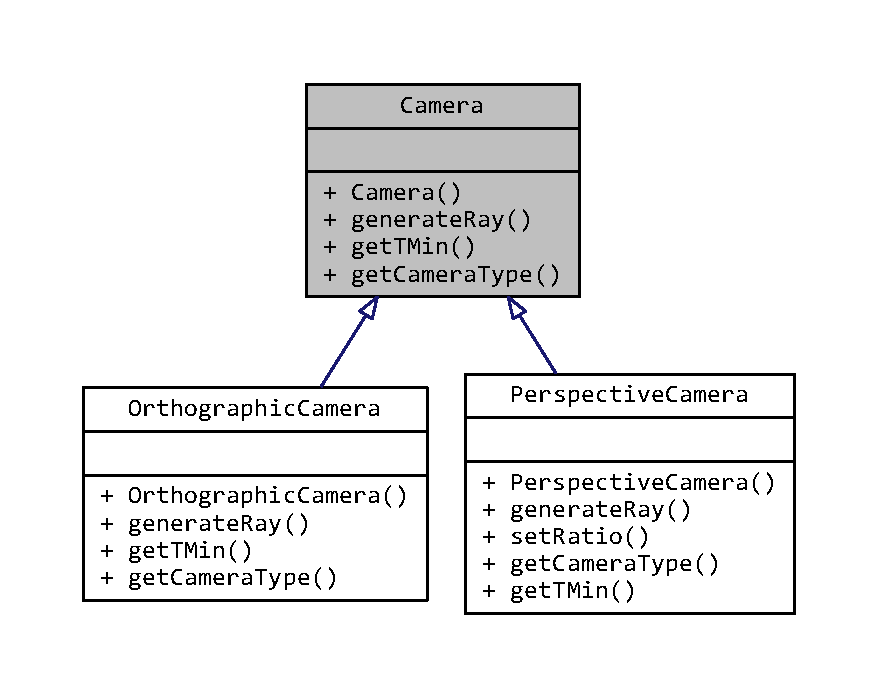
\includegraphics[width=202pt]{classCamera__inherit__graph}
\end{center}
\end{figure}
\subsection*{\-Public \-Member \-Functions}
\begin{DoxyCompactItemize}
\item 
\hypertarget{classCamera_a38dbd2b70b31ee250aadd83b1bbe87fb}{virtual \hyperlink{classRay}{\-Ray} {\bfseries generate\-Ray} (\hyperlink{classVec2f}{\-Vec2f} point)=0}\label{classCamera_a38dbd2b70b31ee250aadd83b1bbe87fb}

\item 
\hypertarget{classCamera_a476000c8588b1aef575482c86153fcb7}{virtual float {\bfseries get\-T\-Min} () const =0}\label{classCamera_a476000c8588b1aef575482c86153fcb7}

\end{DoxyCompactItemize}


\-The documentation for this class was generated from the following file\-:\begin{DoxyCompactItemize}
\item 
\-Camera.\-h\end{DoxyCompactItemize}

\hypertarget{classDirectionalLight}{\section{Directional\+Light Class Reference}
\label{classDirectionalLight}\index{Directional\+Light@{Directional\+Light}}
}


{\ttfamily \#include $<$light.\+h$>$}



Inheritance diagram for Directional\+Light\+:
\nopagebreak
\begin{figure}[H]
\begin{center}
\leavevmode
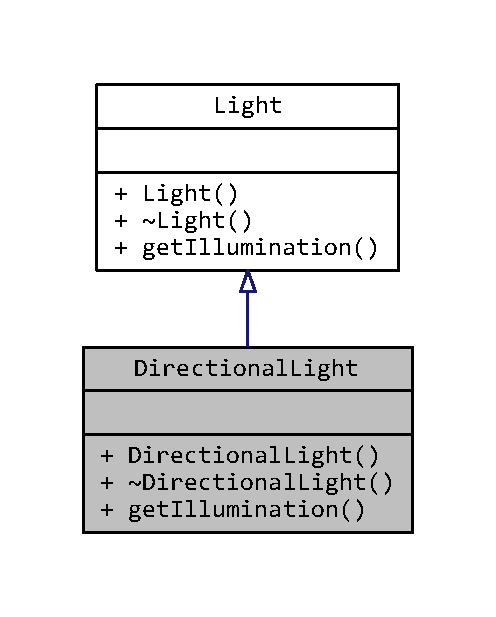
\includegraphics[width=238pt]{classDirectionalLight__inherit__graph}
\end{center}
\end{figure}


Collaboration diagram for Directional\+Light\+:
\nopagebreak
\begin{figure}[H]
\begin{center}
\leavevmode
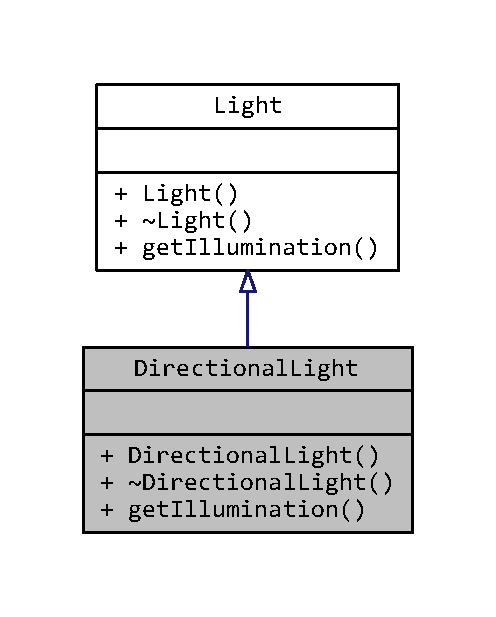
\includegraphics[width=238pt]{classDirectionalLight__coll__graph}
\end{center}
\end{figure}
\subsection*{Public Member Functions}
\begin{DoxyCompactItemize}
\item 
\hyperlink{classDirectionalLight_ab824e6229f84e9c6cd7976f4eb1d99f7}{Directional\+Light} (const \hyperlink{classVec3f}{Vec3f} \&d, const \hyperlink{classVec3f}{Vec3f} \&c)
\item 
\hyperlink{classDirectionalLight_ac4aca6c806e752c65ffea9b2f237b245}{$\sim$\+Directional\+Light} ()
\item 
void \hyperlink{classDirectionalLight_a42ba07f5d908030ad472be265ef13554}{get\+Illumination} (const \hyperlink{classVec3f}{Vec3f} \&p, \hyperlink{classVec3f}{Vec3f} \&dir, \hyperlink{classVec3f}{Vec3f} \&col) const 
\end{DoxyCompactItemize}


\subsection{Constructor \& Destructor Documentation}
\hypertarget{classDirectionalLight_ab824e6229f84e9c6cd7976f4eb1d99f7}{\index{Directional\+Light@{Directional\+Light}!Directional\+Light@{Directional\+Light}}
\index{Directional\+Light@{Directional\+Light}!Directional\+Light@{Directional\+Light}}
\subsubsection[{Directional\+Light}]{\setlength{\rightskip}{0pt plus 5cm}Directional\+Light\+::\+Directional\+Light (
\begin{DoxyParamCaption}
\item[{const {\bf Vec3f} \&}]{d, }
\item[{const {\bf Vec3f} \&}]{c}
\end{DoxyParamCaption}
)\hspace{0.3cm}{\ttfamily [inline]}}}\label{classDirectionalLight_ab824e6229f84e9c6cd7976f4eb1d99f7}
\hypertarget{classDirectionalLight_ac4aca6c806e752c65ffea9b2f237b245}{\index{Directional\+Light@{Directional\+Light}!````~Directional\+Light@{$\sim$\+Directional\+Light}}
\index{````~Directional\+Light@{$\sim$\+Directional\+Light}!Directional\+Light@{Directional\+Light}}
\subsubsection[{$\sim$\+Directional\+Light}]{\setlength{\rightskip}{0pt plus 5cm}Directional\+Light\+::$\sim$\+Directional\+Light (
\begin{DoxyParamCaption}
{}
\end{DoxyParamCaption}
)\hspace{0.3cm}{\ttfamily [inline]}}}\label{classDirectionalLight_ac4aca6c806e752c65ffea9b2f237b245}


\subsection{Member Function Documentation}
\hypertarget{classDirectionalLight_a42ba07f5d908030ad472be265ef13554}{\index{Directional\+Light@{Directional\+Light}!get\+Illumination@{get\+Illumination}}
\index{get\+Illumination@{get\+Illumination}!Directional\+Light@{Directional\+Light}}
\subsubsection[{get\+Illumination}]{\setlength{\rightskip}{0pt plus 5cm}void Directional\+Light\+::get\+Illumination (
\begin{DoxyParamCaption}
\item[{const {\bf Vec3f} \&}]{p, }
\item[{{\bf Vec3f} \&}]{dir, }
\item[{{\bf Vec3f} \&}]{col}
\end{DoxyParamCaption}
) const\hspace{0.3cm}{\ttfamily [inline]}, {\ttfamily [virtual]}}}\label{classDirectionalLight_a42ba07f5d908030ad472be265ef13554}


Implements \hyperlink{classLight_a17e647168f26af631bd687f3c779cd98}{Light}.



The documentation for this class was generated from the following file\+:\begin{DoxyCompactItemize}
\item 
\hyperlink{light_8h}{light.\+h}\end{DoxyCompactItemize}

\hypertarget{classGroup}{\section{Group Class Reference}
\label{classGroup}\index{Group@{Group}}
}


{\ttfamily \#include $<$Group.\+h$>$}



Inheritance diagram for Group\+:
\nopagebreak
\begin{figure}[H]
\begin{center}
\leavevmode
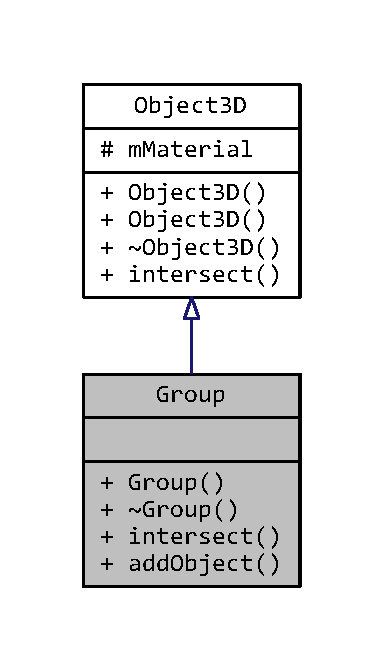
\includegraphics[width=184pt]{classGroup__inherit__graph}
\end{center}
\end{figure}


Collaboration diagram for Group\+:
\nopagebreak
\begin{figure}[H]
\begin{center}
\leavevmode
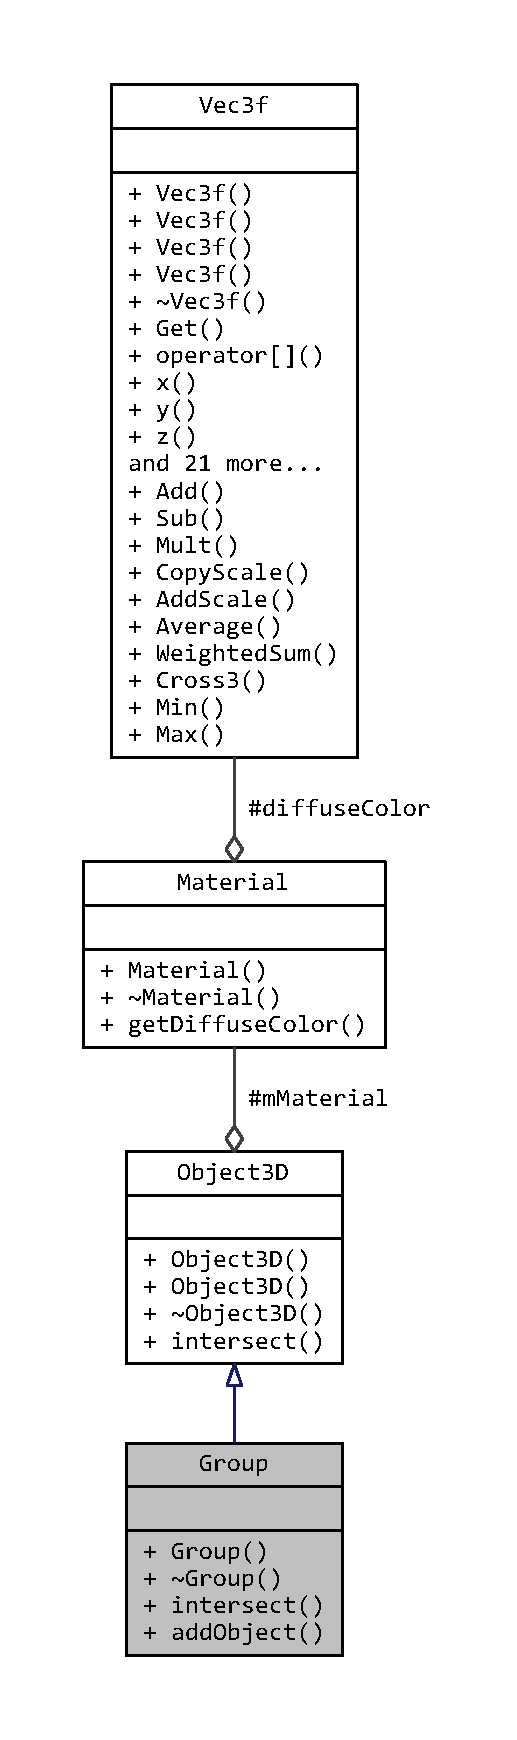
\includegraphics[height=550pt]{classGroup__coll__graph}
\end{center}
\end{figure}
\subsection*{Public Member Functions}
\begin{DoxyCompactItemize}
\item 
\hyperlink{classGroup_aa8b46062ab10d8142daf419be2073c1c}{Group} (int num\+Obj)
\item 
\hyperlink{classGroup_aed00a22ff227ee2657ae44a5cbcedf7c}{$\sim$\+Group} ()
\item 
bool \hyperlink{classGroup_aa09c8e6bce2db3666c1bae2c2fd9688b}{intersect} (const \hyperlink{classRay}{Ray} \&r, \hyperlink{classHit}{Hit} \&h, float tmin)
\item 
void \hyperlink{classGroup_a08dfa34262ba52b8ccf23da53b8482ac}{add\+Object} (int index, \hyperlink{classObject3D}{Object3\+D} $\ast$obj)
\end{DoxyCompactItemize}
\subsection*{Additional Inherited Members}


\subsection{Constructor \& Destructor Documentation}
\hypertarget{classGroup_aa8b46062ab10d8142daf419be2073c1c}{\index{Group@{Group}!Group@{Group}}
\index{Group@{Group}!Group@{Group}}
\subsubsection[{Group}]{\setlength{\rightskip}{0pt plus 5cm}Group\+::\+Group (
\begin{DoxyParamCaption}
\item[{int}]{num\+Obj}
\end{DoxyParamCaption}
)}}\label{classGroup_aa8b46062ab10d8142daf419be2073c1c}
\hypertarget{classGroup_aed00a22ff227ee2657ae44a5cbcedf7c}{\index{Group@{Group}!````~Group@{$\sim$\+Group}}
\index{````~Group@{$\sim$\+Group}!Group@{Group}}
\subsubsection[{$\sim$\+Group}]{\setlength{\rightskip}{0pt plus 5cm}Group\+::$\sim$\+Group (
\begin{DoxyParamCaption}
{}
\end{DoxyParamCaption}
)}}\label{classGroup_aed00a22ff227ee2657ae44a5cbcedf7c}


\subsection{Member Function Documentation}
\hypertarget{classGroup_a08dfa34262ba52b8ccf23da53b8482ac}{\index{Group@{Group}!add\+Object@{add\+Object}}
\index{add\+Object@{add\+Object}!Group@{Group}}
\subsubsection[{add\+Object}]{\setlength{\rightskip}{0pt plus 5cm}void Group\+::add\+Object (
\begin{DoxyParamCaption}
\item[{int}]{index, }
\item[{{\bf Object3\+D} $\ast$}]{obj}
\end{DoxyParamCaption}
)}}\label{classGroup_a08dfa34262ba52b8ccf23da53b8482ac}
\hypertarget{classGroup_aa09c8e6bce2db3666c1bae2c2fd9688b}{\index{Group@{Group}!intersect@{intersect}}
\index{intersect@{intersect}!Group@{Group}}
\subsubsection[{intersect}]{\setlength{\rightskip}{0pt plus 5cm}bool Group\+::intersect (
\begin{DoxyParamCaption}
\item[{const {\bf Ray} \&}]{r, }
\item[{{\bf Hit} \&}]{h, }
\item[{float}]{tmin}
\end{DoxyParamCaption}
)\hspace{0.3cm}{\ttfamily [virtual]}}}\label{classGroup_aa09c8e6bce2db3666c1bae2c2fd9688b}


Implements \hyperlink{classObject3D_a58f07cf2b37c5b6a1c796cd7a939f91b}{Object3\+D}.



The documentation for this class was generated from the following files\+:\begin{DoxyCompactItemize}
\item 
\hyperlink{Group_8h}{Group.\+h}\item 
\hyperlink{Group_8cpp}{Group.\+cpp}\end{DoxyCompactItemize}

\hypertarget{classHit}{\section{Hit Class Reference}
\label{classHit}\index{Hit@{Hit}}
}


{\ttfamily \#include $<$hit.\+h$>$}



Collaboration diagram for Hit\+:
\nopagebreak
\begin{figure}[H]
\begin{center}
\leavevmode
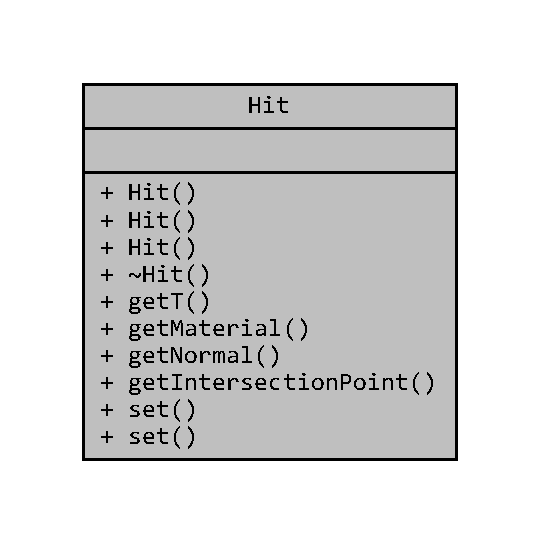
\includegraphics[width=259pt]{classHit__coll__graph}
\end{center}
\end{figure}
\subsection*{Public Member Functions}
\begin{DoxyCompactItemize}
\item 
\hyperlink{classHit_ac2727a27933c07b60b6a7ccccba12fff}{Hit} ()
\item 
\hyperlink{classHit_a5a32f693b7c37fedfc0d2b357b03374a}{Hit} (float \+\_\+t, \hyperlink{classMaterial}{Material} $\ast$m, \hyperlink{classVec3f}{Vec3f} n)
\item 
\hyperlink{classHit_acb4d552eb2451c8310329e485a516d06}{Hit} (const \hyperlink{classHit}{Hit} \&h)
\item 
\hyperlink{classHit_a6b06024fcf4bc21acd339461a549dc7c}{$\sim$\+Hit} ()
\item 
float \hyperlink{classHit_af5ebbf2d4370f17826617ea7d441abd9}{get\+T} () const 
\item 
\hyperlink{classMaterial}{Material} $\ast$ \hyperlink{classHit_a8143afec295fb4418daf38d207692923}{get\+Material} () const 
\item 
\hyperlink{classVec3f}{Vec3f} \hyperlink{classHit_aaa0cbcac47165d07318bba5efdb574f2}{get\+Normal} () const 
\item 
\hyperlink{classVec3f}{Vec3f} \hyperlink{classHit_ac07b2cc6a362e066abc87b86ff4c281d}{get\+Intersection\+Point} () const 
\item 
void \hyperlink{classHit_a09dd5834765113b153e12665ec580d36}{set} (float \+\_\+t, \hyperlink{classMaterial}{Material} $\ast$m, \hyperlink{classVec3f}{Vec3f} n, const \hyperlink{classRay}{Ray} \&ray)
\item 
void \hyperlink{classHit_acb2283496ca855ff94de46f4058ab1b8}{set} (float \+\_\+t, \hyperlink{classMaterial}{Material} $\ast$m, \hyperlink{classVec3f}{Vec3f} n, const \hyperlink{classVec3f}{Vec3f} \&p)
\end{DoxyCompactItemize}


\subsection{Constructor \& Destructor Documentation}
\hypertarget{classHit_ac2727a27933c07b60b6a7ccccba12fff}{\index{Hit@{Hit}!Hit@{Hit}}
\index{Hit@{Hit}!Hit@{Hit}}
\subsubsection[{Hit}]{\setlength{\rightskip}{0pt plus 5cm}Hit\+::\+Hit (
\begin{DoxyParamCaption}
{}
\end{DoxyParamCaption}
)\hspace{0.3cm}{\ttfamily [inline]}}}\label{classHit_ac2727a27933c07b60b6a7ccccba12fff}
\hypertarget{classHit_a5a32f693b7c37fedfc0d2b357b03374a}{\index{Hit@{Hit}!Hit@{Hit}}
\index{Hit@{Hit}!Hit@{Hit}}
\subsubsection[{Hit}]{\setlength{\rightskip}{0pt plus 5cm}Hit\+::\+Hit (
\begin{DoxyParamCaption}
\item[{float}]{\+\_\+t, }
\item[{{\bf Material} $\ast$}]{m, }
\item[{{\bf Vec3f}}]{n}
\end{DoxyParamCaption}
)\hspace{0.3cm}{\ttfamily [inline]}}}\label{classHit_a5a32f693b7c37fedfc0d2b357b03374a}
\hypertarget{classHit_acb4d552eb2451c8310329e485a516d06}{\index{Hit@{Hit}!Hit@{Hit}}
\index{Hit@{Hit}!Hit@{Hit}}
\subsubsection[{Hit}]{\setlength{\rightskip}{0pt plus 5cm}Hit\+::\+Hit (
\begin{DoxyParamCaption}
\item[{const {\bf Hit} \&}]{h}
\end{DoxyParamCaption}
)\hspace{0.3cm}{\ttfamily [inline]}}}\label{classHit_acb4d552eb2451c8310329e485a516d06}
\hypertarget{classHit_a6b06024fcf4bc21acd339461a549dc7c}{\index{Hit@{Hit}!````~Hit@{$\sim$\+Hit}}
\index{````~Hit@{$\sim$\+Hit}!Hit@{Hit}}
\subsubsection[{$\sim$\+Hit}]{\setlength{\rightskip}{0pt plus 5cm}Hit\+::$\sim$\+Hit (
\begin{DoxyParamCaption}
{}
\end{DoxyParamCaption}
)\hspace{0.3cm}{\ttfamily [inline]}}}\label{classHit_a6b06024fcf4bc21acd339461a549dc7c}


\subsection{Member Function Documentation}
\hypertarget{classHit_ac07b2cc6a362e066abc87b86ff4c281d}{\index{Hit@{Hit}!get\+Intersection\+Point@{get\+Intersection\+Point}}
\index{get\+Intersection\+Point@{get\+Intersection\+Point}!Hit@{Hit}}
\subsubsection[{get\+Intersection\+Point}]{\setlength{\rightskip}{0pt plus 5cm}{\bf Vec3f} Hit\+::get\+Intersection\+Point (
\begin{DoxyParamCaption}
{}
\end{DoxyParamCaption}
) const\hspace{0.3cm}{\ttfamily [inline]}}}\label{classHit_ac07b2cc6a362e066abc87b86ff4c281d}
\hypertarget{classHit_a8143afec295fb4418daf38d207692923}{\index{Hit@{Hit}!get\+Material@{get\+Material}}
\index{get\+Material@{get\+Material}!Hit@{Hit}}
\subsubsection[{get\+Material}]{\setlength{\rightskip}{0pt plus 5cm}{\bf Material}$\ast$ Hit\+::get\+Material (
\begin{DoxyParamCaption}
{}
\end{DoxyParamCaption}
) const\hspace{0.3cm}{\ttfamily [inline]}}}\label{classHit_a8143afec295fb4418daf38d207692923}
\hypertarget{classHit_aaa0cbcac47165d07318bba5efdb574f2}{\index{Hit@{Hit}!get\+Normal@{get\+Normal}}
\index{get\+Normal@{get\+Normal}!Hit@{Hit}}
\subsubsection[{get\+Normal}]{\setlength{\rightskip}{0pt plus 5cm}{\bf Vec3f} Hit\+::get\+Normal (
\begin{DoxyParamCaption}
{}
\end{DoxyParamCaption}
) const\hspace{0.3cm}{\ttfamily [inline]}}}\label{classHit_aaa0cbcac47165d07318bba5efdb574f2}
\hypertarget{classHit_af5ebbf2d4370f17826617ea7d441abd9}{\index{Hit@{Hit}!get\+T@{get\+T}}
\index{get\+T@{get\+T}!Hit@{Hit}}
\subsubsection[{get\+T}]{\setlength{\rightskip}{0pt plus 5cm}float Hit\+::get\+T (
\begin{DoxyParamCaption}
{}
\end{DoxyParamCaption}
) const\hspace{0.3cm}{\ttfamily [inline]}}}\label{classHit_af5ebbf2d4370f17826617ea7d441abd9}
\hypertarget{classHit_a09dd5834765113b153e12665ec580d36}{\index{Hit@{Hit}!set@{set}}
\index{set@{set}!Hit@{Hit}}
\subsubsection[{set}]{\setlength{\rightskip}{0pt plus 5cm}void Hit\+::set (
\begin{DoxyParamCaption}
\item[{float}]{\+\_\+t, }
\item[{{\bf Material} $\ast$}]{m, }
\item[{{\bf Vec3f}}]{n, }
\item[{const {\bf Ray} \&}]{ray}
\end{DoxyParamCaption}
)\hspace{0.3cm}{\ttfamily [inline]}}}\label{classHit_a09dd5834765113b153e12665ec580d36}
\hypertarget{classHit_acb2283496ca855ff94de46f4058ab1b8}{\index{Hit@{Hit}!set@{set}}
\index{set@{set}!Hit@{Hit}}
\subsubsection[{set}]{\setlength{\rightskip}{0pt plus 5cm}void Hit\+::set (
\begin{DoxyParamCaption}
\item[{float}]{\+\_\+t, }
\item[{{\bf Material} $\ast$}]{m, }
\item[{{\bf Vec3f}}]{n, }
\item[{const {\bf Vec3f} \&}]{p}
\end{DoxyParamCaption}
)\hspace{0.3cm}{\ttfamily [inline]}}}\label{classHit_acb2283496ca855ff94de46f4058ab1b8}


The documentation for this class was generated from the following file\+:\begin{DoxyCompactItemize}
\item 
\hyperlink{hit_8h}{hit.\+h}\end{DoxyCompactItemize}

\hypertarget{classImage}{\section{\-Image \-Class \-Reference}
\label{classImage}\index{\-Image@{\-Image}}
}
\subsection*{\-Public \-Member \-Functions}
\begin{DoxyCompactItemize}
\item 
\hypertarget{classImage_a05c964ca59502cc32c30e8ab89b5e920}{{\bfseries \-Image} (int w, int h)}\label{classImage_a05c964ca59502cc32c30e8ab89b5e920}

\item 
\hypertarget{classImage_a55e9332ab0f27716de2b0765e1134aeb}{int {\bfseries \-Width} () const }\label{classImage_a55e9332ab0f27716de2b0765e1134aeb}

\item 
\hypertarget{classImage_a4ba2103cb0db707dabaea6adbab00be7}{int {\bfseries \-Height} () const }\label{classImage_a4ba2103cb0db707dabaea6adbab00be7}

\item 
\hypertarget{classImage_a5902ab3207a0d6f5b8fe92b6f11cb292}{const \hyperlink{classVec3f}{\-Vec3f} \& {\bfseries \-Get\-Pixel} (int x, int y) const }\label{classImage_a5902ab3207a0d6f5b8fe92b6f11cb292}

\item 
\hypertarget{classImage_a4e91934550b21dd19041ea144e498c3c}{void {\bfseries \-Set\-All\-Pixels} (const \hyperlink{classVec3f}{\-Vec3f} \&color)}\label{classImage_a4e91934550b21dd19041ea144e498c3c}

\item 
\hypertarget{classImage_af2f04f2fe7e6c3aba0401a0c6515963a}{void {\bfseries \-Set\-Pixel} (int x, int y, const \hyperlink{classVec3f}{\-Vec3f} \&color)}\label{classImage_af2f04f2fe7e6c3aba0401a0c6515963a}

\item 
\hypertarget{classImage_a7aeb4943c2f410f9a806e91eb917756d}{void {\bfseries \-Save\-P\-P\-M} (const char $\ast$filename) const }\label{classImage_a7aeb4943c2f410f9a806e91eb917756d}

\item 
\hypertarget{classImage_a12ab68b68cc0f9c6501d2b4a019eb564}{void {\bfseries \-Save\-T\-G\-A} (const char $\ast$filename) const }\label{classImage_a12ab68b68cc0f9c6501d2b4a019eb564}

\end{DoxyCompactItemize}
\subsection*{\-Static \-Public \-Member \-Functions}
\begin{DoxyCompactItemize}
\item 
\hypertarget{classImage_ac2fc9197cc697efa2c610efe0519b466}{static \hyperlink{classImage}{\-Image} $\ast$ {\bfseries \-Load\-P\-P\-M} (const char $\ast$filename)}\label{classImage_ac2fc9197cc697efa2c610efe0519b466}

\item 
\hypertarget{classImage_a7c6b50633e25f53f9c5f1af90bf8332b}{static \hyperlink{classImage}{\-Image} $\ast$ {\bfseries \-Load\-T\-G\-A} (const char $\ast$filename)}\label{classImage_a7c6b50633e25f53f9c5f1af90bf8332b}

\item 
\hypertarget{classImage_ac025574f36e212489546450083f3d331}{static \hyperlink{classImage}{\-Image} $\ast$ {\bfseries \-Compare} (\hyperlink{classImage}{\-Image} $\ast$img1, \hyperlink{classImage}{\-Image} $\ast$img2)}\label{classImage_ac025574f36e212489546450083f3d331}

\end{DoxyCompactItemize}


\-The documentation for this class was generated from the following files\-:\begin{DoxyCompactItemize}
\item 
image.\-h\item 
image.\-cpp\end{DoxyCompactItemize}

\hypertarget{classLight}{\section{Light Class Reference}
\label{classLight}\index{Light@{Light}}
}


{\ttfamily \#include $<$light.\+h$>$}



Inheritance diagram for Light\+:
\nopagebreak
\begin{figure}[H]
\begin{center}
\leavevmode
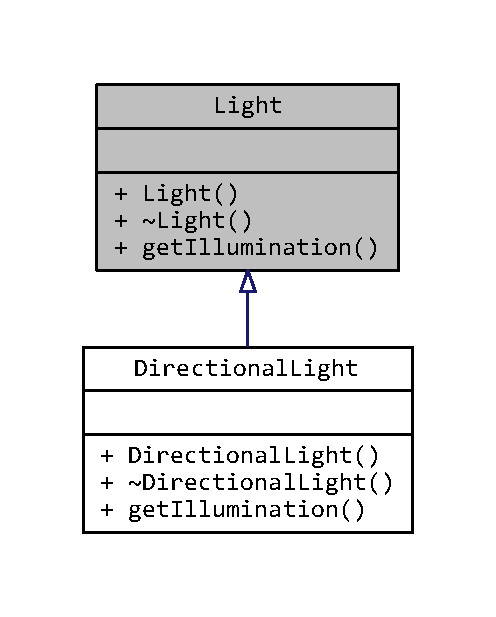
\includegraphics[width=238pt]{classLight__inherit__graph}
\end{center}
\end{figure}


Collaboration diagram for Light\+:
\nopagebreak
\begin{figure}[H]
\begin{center}
\leavevmode
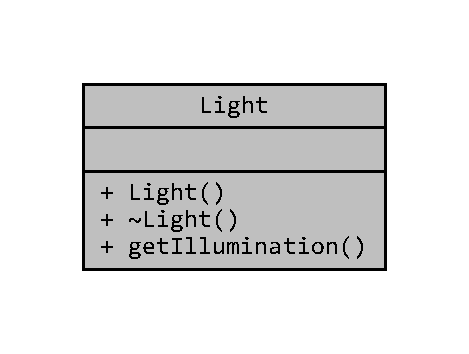
\includegraphics[width=225pt]{classLight__coll__graph}
\end{center}
\end{figure}
\subsection*{Public Member Functions}
\begin{DoxyCompactItemize}
\item 
\hyperlink{classLight_aeb5df09a25a32f19fdffa761268ba24f}{Light} ()
\item 
virtual \hyperlink{classLight_abe675054027c4b4a4f3e9a31d330931f}{$\sim$\+Light} ()
\item 
virtual void \hyperlink{classLight_a17e647168f26af631bd687f3c779cd98}{get\+Illumination} (const \hyperlink{classVec3f}{Vec3f} \&p, \hyperlink{classVec3f}{Vec3f} \&dir, \hyperlink{classVec3f}{Vec3f} \&col) const =0
\end{DoxyCompactItemize}


\subsection{Constructor \& Destructor Documentation}
\hypertarget{classLight_aeb5df09a25a32f19fdffa761268ba24f}{\index{Light@{Light}!Light@{Light}}
\index{Light@{Light}!Light@{Light}}
\subsubsection[{Light}]{\setlength{\rightskip}{0pt plus 5cm}Light\+::\+Light (
\begin{DoxyParamCaption}
{}
\end{DoxyParamCaption}
)\hspace{0.3cm}{\ttfamily [inline]}}}\label{classLight_aeb5df09a25a32f19fdffa761268ba24f}
\hypertarget{classLight_abe675054027c4b4a4f3e9a31d330931f}{\index{Light@{Light}!````~Light@{$\sim$\+Light}}
\index{````~Light@{$\sim$\+Light}!Light@{Light}}
\subsubsection[{$\sim$\+Light}]{\setlength{\rightskip}{0pt plus 5cm}virtual Light\+::$\sim$\+Light (
\begin{DoxyParamCaption}
{}
\end{DoxyParamCaption}
)\hspace{0.3cm}{\ttfamily [inline]}, {\ttfamily [virtual]}}}\label{classLight_abe675054027c4b4a4f3e9a31d330931f}


\subsection{Member Function Documentation}
\hypertarget{classLight_a17e647168f26af631bd687f3c779cd98}{\index{Light@{Light}!get\+Illumination@{get\+Illumination}}
\index{get\+Illumination@{get\+Illumination}!Light@{Light}}
\subsubsection[{get\+Illumination}]{\setlength{\rightskip}{0pt plus 5cm}virtual void Light\+::get\+Illumination (
\begin{DoxyParamCaption}
\item[{const {\bf Vec3f} \&}]{p, }
\item[{{\bf Vec3f} \&}]{dir, }
\item[{{\bf Vec3f} \&}]{col}
\end{DoxyParamCaption}
) const\hspace{0.3cm}{\ttfamily [pure virtual]}}}\label{classLight_a17e647168f26af631bd687f3c779cd98}


Implemented in \hyperlink{classDirectionalLight_a42ba07f5d908030ad472be265ef13554}{Directional\+Light}.



The documentation for this class was generated from the following file\+:\begin{DoxyCompactItemize}
\item 
\hyperlink{light_8h}{light.\+h}\end{DoxyCompactItemize}

\hypertarget{classMaterial}{\section{Material Class Reference}
\label{classMaterial}\index{Material@{Material}}
}


{\ttfamily \#include $<$material.\+h$>$}



Collaboration diagram for Material\+:
\nopagebreak
\begin{figure}[H]
\begin{center}
\leavevmode
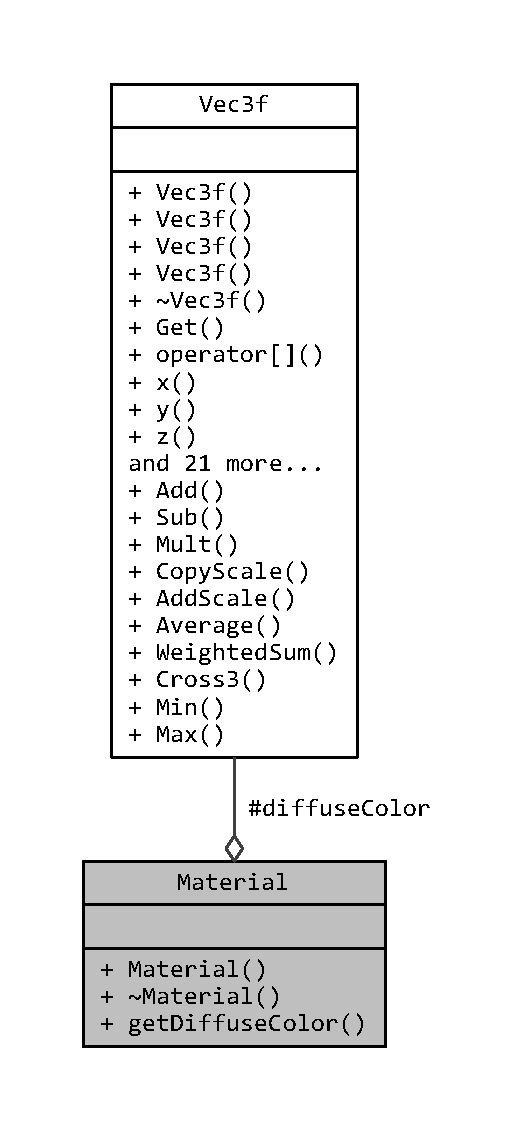
\includegraphics[width=248pt]{classMaterial__coll__graph}
\end{center}
\end{figure}
\subsection*{Public Member Functions}
\begin{DoxyCompactItemize}
\item 
\hyperlink{classMaterial_a35eb3afb51f8d1425df2da47e8030fad}{Material} (const \hyperlink{classVec3f}{Vec3f} \&d\+\_\+color)
\item 
virtual \hyperlink{classMaterial_a179e16d6a1bd4a0f039b8e4cbf2ade30}{$\sim$\+Material} ()
\item 
virtual \hyperlink{classVec3f}{Vec3f} \hyperlink{classMaterial_a83b7c9dcae7d529879d90c920892e611}{get\+Diffuse\+Color} () const 
\end{DoxyCompactItemize}
\subsection*{Protected Attributes}
\begin{DoxyCompactItemize}
\item 
\hyperlink{classVec3f}{Vec3f} \hyperlink{classMaterial_ae81bccaee22b88d46074b843dc7bdc32}{diffuse\+Color}
\end{DoxyCompactItemize}


\subsection{Constructor \& Destructor Documentation}
\hypertarget{classMaterial_a35eb3afb51f8d1425df2da47e8030fad}{\index{Material@{Material}!Material@{Material}}
\index{Material@{Material}!Material@{Material}}
\subsubsection[{Material}]{\setlength{\rightskip}{0pt plus 5cm}Material\+::\+Material (
\begin{DoxyParamCaption}
\item[{const {\bf Vec3f} \&}]{d\+\_\+color}
\end{DoxyParamCaption}
)\hspace{0.3cm}{\ttfamily [inline]}}}\label{classMaterial_a35eb3afb51f8d1425df2da47e8030fad}
\hypertarget{classMaterial_a179e16d6a1bd4a0f039b8e4cbf2ade30}{\index{Material@{Material}!````~Material@{$\sim$\+Material}}
\index{````~Material@{$\sim$\+Material}!Material@{Material}}
\subsubsection[{$\sim$\+Material}]{\setlength{\rightskip}{0pt plus 5cm}virtual Material\+::$\sim$\+Material (
\begin{DoxyParamCaption}
{}
\end{DoxyParamCaption}
)\hspace{0.3cm}{\ttfamily [inline]}, {\ttfamily [virtual]}}}\label{classMaterial_a179e16d6a1bd4a0f039b8e4cbf2ade30}


\subsection{Member Function Documentation}
\hypertarget{classMaterial_a83b7c9dcae7d529879d90c920892e611}{\index{Material@{Material}!get\+Diffuse\+Color@{get\+Diffuse\+Color}}
\index{get\+Diffuse\+Color@{get\+Diffuse\+Color}!Material@{Material}}
\subsubsection[{get\+Diffuse\+Color}]{\setlength{\rightskip}{0pt plus 5cm}virtual {\bf Vec3f} Material\+::get\+Diffuse\+Color (
\begin{DoxyParamCaption}
{}
\end{DoxyParamCaption}
) const\hspace{0.3cm}{\ttfamily [inline]}, {\ttfamily [virtual]}}}\label{classMaterial_a83b7c9dcae7d529879d90c920892e611}


\subsection{Member Data Documentation}
\hypertarget{classMaterial_ae81bccaee22b88d46074b843dc7bdc32}{\index{Material@{Material}!diffuse\+Color@{diffuse\+Color}}
\index{diffuse\+Color@{diffuse\+Color}!Material@{Material}}
\subsubsection[{diffuse\+Color}]{\setlength{\rightskip}{0pt plus 5cm}{\bf Vec3f} Material\+::diffuse\+Color\hspace{0.3cm}{\ttfamily [protected]}}}\label{classMaterial_ae81bccaee22b88d46074b843dc7bdc32}


The documentation for this class was generated from the following file\+:\begin{DoxyCompactItemize}
\item 
\hyperlink{material_8h}{material.\+h}\end{DoxyCompactItemize}

\hypertarget{classMatrix}{\section{Matrix Class Reference}
\label{classMatrix}\index{Matrix@{Matrix}}
}


{\ttfamily \#include $<$matrix.\+h$>$}



Collaboration diagram for Matrix\+:
\nopagebreak
\begin{figure}[H]
\begin{center}
\leavevmode
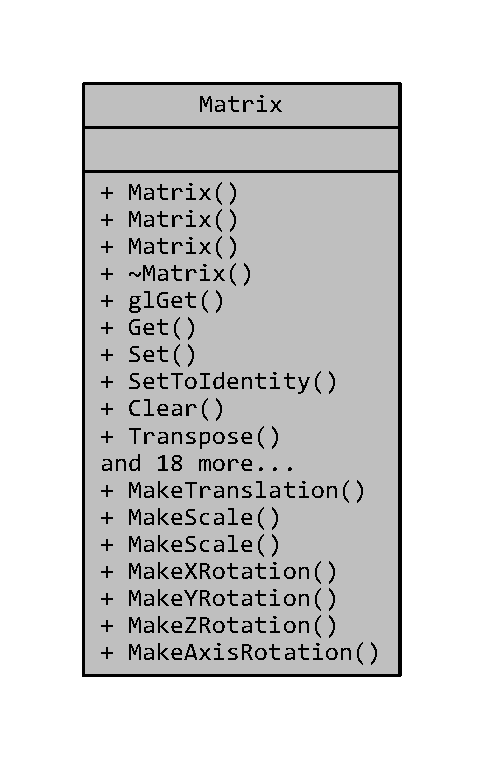
\includegraphics[width=232pt]{classMatrix__coll__graph}
\end{center}
\end{figure}
\subsection*{Public Member Functions}
\begin{DoxyCompactItemize}
\item 
\hyperlink{classMatrix_a2dba13c45127354c9f75ef576f49269b}{Matrix} ()
\item 
\hyperlink{classMatrix_a765f4dcb51b6829311cc3e7576388423}{Matrix} (const \hyperlink{classMatrix}{Matrix} \&m)
\item 
\hyperlink{classMatrix_acfc1445f8a381d32f1989cd35714c290}{Matrix} (const float $\ast$m)
\item 
\hyperlink{classMatrix_a9b1c3627f573d78a2f08623fdfef990f}{$\sim$\+Matrix} ()
\item 
float $\ast$ \hyperlink{classMatrix_af8d06eec2ed4cc9329d664d539c7f2b8}{gl\+Get} (void) const 
\item 
float \hyperlink{classMatrix_aef91dcc82ede72fd100dc3e4004234c7}{Get} (int x, int y) const 
\item 
void \hyperlink{classMatrix_ac3560c1c5173148d2ed77488e46bd79f}{Set} (int x, int y, float v)
\item 
void \hyperlink{classMatrix_a16343771112fd6a54e6f3383bd82598d}{Set\+To\+Identity} ()
\item 
void \hyperlink{classMatrix_a77024c11b6ff4b02a265bfda0ff7eab1}{Clear} ()
\item 
void \hyperlink{classMatrix_a8191ef7491d6caa30bc367ec7c64cf30}{Transpose} (\hyperlink{classMatrix}{Matrix} \&m) const 
\item 
void \hyperlink{classMatrix_a350d12361c31ec650e667e8120da7274}{Transpose} ()
\item 
int \hyperlink{classMatrix_a84db3b710d89b69bf7fe5c019185fbbb}{Inverse} (\hyperlink{classMatrix}{Matrix} \&m, float epsilon=1e-\/08) const 
\item 
int \hyperlink{classMatrix_af203ab3d087288d9eb6e84afe5814fa9}{Inverse} (float epsilon=1e-\/08)
\item 
\hyperlink{classMatrix}{Matrix} \& \hyperlink{classMatrix_aea5a06385f646eb4a63929fae6fa3e14}{operator=} (const \hyperlink{classMatrix}{Matrix} \&m)
\item 
int \hyperlink{classMatrix_a3907074da7d66966da2ae99413d1c3bf}{operator==} (const \hyperlink{classMatrix}{Matrix} \&m) const 
\item 
int \hyperlink{classMatrix_a7677246e5e4d8350758f4f651dc87c90}{operator!=} (const \hyperlink{classMatrix}{Matrix} \&m) const 
\item 
\hyperlink{classMatrix}{Matrix} \& \hyperlink{classMatrix_a2780b459599c6ba0b4c63ce6ca6c1ba9}{operator+=} (const \hyperlink{classMatrix}{Matrix} \&m)
\item 
\hyperlink{classMatrix}{Matrix} \& \hyperlink{classMatrix_a26bb57b9a95c3c5ddcb6dfe4de089f04}{operator-\/=} (const \hyperlink{classMatrix}{Matrix} \&m)
\item 
\hyperlink{classMatrix}{Matrix} \& \hyperlink{classMatrix_a2db81df6efad774392a12384f7c2cf26}{operator$\ast$=} (const float f)
\item 
\hyperlink{classMatrix}{Matrix} \& \hyperlink{classMatrix_a4680eaaf820efafb0017a2ee593bea8c}{operator$\ast$=} (const \hyperlink{classMatrix}{Matrix} \&m)
\item 
void \hyperlink{classMatrix_a815a83fda075f44bf71f13defca9f83e}{Transform} (\hyperlink{classVec4f}{Vec4f} \&v) const 
\item 
void \hyperlink{classMatrix_a7208989bf27372bb361390c4b4df2157}{Transform} (\hyperlink{classVec3f}{Vec3f} \&v) const 
\item 
void \hyperlink{classMatrix_a16f9a1cf796c64979de415ba161ef84c}{Transform} (\hyperlink{classVec2f}{Vec2f} \&v) const 
\item 
void \hyperlink{classMatrix_a21f46ddfd67d21e873076e468f9b793e}{Transform\+Direction} (\hyperlink{classVec3f}{Vec3f} \&v) const 
\item 
void \hyperlink{classMatrix_ae8ba2f4d4b1431f5a0a9b77e654a544f}{Write} (F\+I\+L\+E $\ast$F=stdout) const 
\item 
void \hyperlink{classMatrix_a2c6c2fd2c666999a410ebccbd510d4fe}{Write3x3} (F\+I\+L\+E $\ast$F=stdout) const 
\item 
void \hyperlink{classMatrix_a6b4caf9e67b3981b432a7d7ea33530fa}{Read} (F\+I\+L\+E $\ast$F)
\item 
void \hyperlink{classMatrix_aa9884c4699079277f126cbaef4b76df6}{Read3x3} (F\+I\+L\+E $\ast$F)
\end{DoxyCompactItemize}
\subsection*{Static Public Member Functions}
\begin{DoxyCompactItemize}
\item 
static \hyperlink{classMatrix}{Matrix} \hyperlink{classMatrix_a2b1cb490a87242c87a70663740da4ec5}{Make\+Translation} (const \hyperlink{classVec3f}{Vec3f} \&v)
\item 
static \hyperlink{classMatrix}{Matrix} \hyperlink{classMatrix_abf53a10add62314631229fc752cd8c84}{Make\+Scale} (const \hyperlink{classVec3f}{Vec3f} \&v)
\item 
static \hyperlink{classMatrix}{Matrix} \hyperlink{classMatrix_a503eab51a48058e56e60b6199bb1b8e8}{Make\+Scale} (float s)
\item 
static \hyperlink{classMatrix}{Matrix} \hyperlink{classMatrix_a2e1addd0f882e4ce73264258525f70e0}{Make\+X\+Rotation} (float theta)
\item 
static \hyperlink{classMatrix}{Matrix} \hyperlink{classMatrix_a0848f661169a85ca7ee24f1d7b30aa80}{Make\+Y\+Rotation} (float theta)
\item 
static \hyperlink{classMatrix}{Matrix} \hyperlink{classMatrix_a10fcfa34357b477fd80c25b31e2d9105}{Make\+Z\+Rotation} (float theta)
\item 
static \hyperlink{classMatrix}{Matrix} \hyperlink{classMatrix_a2134c6c917c3bf24797c1202f56d9e82}{Make\+Axis\+Rotation} (const \hyperlink{classVec3f}{Vec3f} \&v, float theta)
\end{DoxyCompactItemize}
\subsection*{Friends}
\begin{DoxyCompactItemize}
\item 
\hyperlink{classMatrix}{Matrix} \hyperlink{classMatrix_aa5a9f2db2b3c1862c9c0d19241239ce7}{operator+} (const \hyperlink{classMatrix}{Matrix} \&m1, const \hyperlink{classMatrix}{Matrix} \&m2)
\item 
\hyperlink{classMatrix}{Matrix} \hyperlink{classMatrix_a52ad5ef4b9998529c85e8523c20d6b86}{operator-\/} (const \hyperlink{classMatrix}{Matrix} \&m1, const \hyperlink{classMatrix}{Matrix} \&m2)
\item 
\hyperlink{classMatrix}{Matrix} \hyperlink{classMatrix_a24da5fd1a21f5010ee32de71af9be3b9}{operator$\ast$} (const \hyperlink{classMatrix}{Matrix} \&m1, const \hyperlink{classMatrix}{Matrix} \&m2)
\item 
\hyperlink{classMatrix}{Matrix} \hyperlink{classMatrix_a895d86a3588e50c3aa51f0e43b43de39}{operator$\ast$} (const \hyperlink{classMatrix}{Matrix} \&m1, float f)
\item 
\hyperlink{classMatrix}{Matrix} \hyperlink{classMatrix_a900892d8498953af4e4606741601c017}{operator$\ast$} (float f, const \hyperlink{classMatrix}{Matrix} \&m)
\end{DoxyCompactItemize}


\subsection{Constructor \& Destructor Documentation}
\hypertarget{classMatrix_a2dba13c45127354c9f75ef576f49269b}{\index{Matrix@{Matrix}!Matrix@{Matrix}}
\index{Matrix@{Matrix}!Matrix@{Matrix}}
\subsubsection[{Matrix}]{\setlength{\rightskip}{0pt plus 5cm}Matrix\+::\+Matrix (
\begin{DoxyParamCaption}
{}
\end{DoxyParamCaption}
)\hspace{0.3cm}{\ttfamily [inline]}}}\label{classMatrix_a2dba13c45127354c9f75ef576f49269b}
\hypertarget{classMatrix_a765f4dcb51b6829311cc3e7576388423}{\index{Matrix@{Matrix}!Matrix@{Matrix}}
\index{Matrix@{Matrix}!Matrix@{Matrix}}
\subsubsection[{Matrix}]{\setlength{\rightskip}{0pt plus 5cm}Matrix\+::\+Matrix (
\begin{DoxyParamCaption}
\item[{const {\bf Matrix} \&}]{m}
\end{DoxyParamCaption}
)}}\label{classMatrix_a765f4dcb51b6829311cc3e7576388423}
\hypertarget{classMatrix_acfc1445f8a381d32f1989cd35714c290}{\index{Matrix@{Matrix}!Matrix@{Matrix}}
\index{Matrix@{Matrix}!Matrix@{Matrix}}
\subsubsection[{Matrix}]{\setlength{\rightskip}{0pt plus 5cm}Matrix\+::\+Matrix (
\begin{DoxyParamCaption}
\item[{const float $\ast$}]{m}
\end{DoxyParamCaption}
)}}\label{classMatrix_acfc1445f8a381d32f1989cd35714c290}
\hypertarget{classMatrix_a9b1c3627f573d78a2f08623fdfef990f}{\index{Matrix@{Matrix}!````~Matrix@{$\sim$\+Matrix}}
\index{````~Matrix@{$\sim$\+Matrix}!Matrix@{Matrix}}
\subsubsection[{$\sim$\+Matrix}]{\setlength{\rightskip}{0pt plus 5cm}Matrix\+::$\sim$\+Matrix (
\begin{DoxyParamCaption}
{}
\end{DoxyParamCaption}
)\hspace{0.3cm}{\ttfamily [inline]}}}\label{classMatrix_a9b1c3627f573d78a2f08623fdfef990f}


\subsection{Member Function Documentation}
\hypertarget{classMatrix_a77024c11b6ff4b02a265bfda0ff7eab1}{\index{Matrix@{Matrix}!Clear@{Clear}}
\index{Clear@{Clear}!Matrix@{Matrix}}
\subsubsection[{Clear}]{\setlength{\rightskip}{0pt plus 5cm}void Matrix\+::\+Clear (
\begin{DoxyParamCaption}
{}
\end{DoxyParamCaption}
)}}\label{classMatrix_a77024c11b6ff4b02a265bfda0ff7eab1}
\hypertarget{classMatrix_aef91dcc82ede72fd100dc3e4004234c7}{\index{Matrix@{Matrix}!Get@{Get}}
\index{Get@{Get}!Matrix@{Matrix}}
\subsubsection[{Get}]{\setlength{\rightskip}{0pt plus 5cm}float Matrix\+::\+Get (
\begin{DoxyParamCaption}
\item[{int}]{x, }
\item[{int}]{y}
\end{DoxyParamCaption}
) const\hspace{0.3cm}{\ttfamily [inline]}}}\label{classMatrix_aef91dcc82ede72fd100dc3e4004234c7}
\hypertarget{classMatrix_af8d06eec2ed4cc9329d664d539c7f2b8}{\index{Matrix@{Matrix}!gl\+Get@{gl\+Get}}
\index{gl\+Get@{gl\+Get}!Matrix@{Matrix}}
\subsubsection[{gl\+Get}]{\setlength{\rightskip}{0pt plus 5cm}float$\ast$ Matrix\+::gl\+Get (
\begin{DoxyParamCaption}
\item[{void}]{}
\end{DoxyParamCaption}
) const\hspace{0.3cm}{\ttfamily [inline]}}}\label{classMatrix_af8d06eec2ed4cc9329d664d539c7f2b8}
\hypertarget{classMatrix_a84db3b710d89b69bf7fe5c019185fbbb}{\index{Matrix@{Matrix}!Inverse@{Inverse}}
\index{Inverse@{Inverse}!Matrix@{Matrix}}
\subsubsection[{Inverse}]{\setlength{\rightskip}{0pt plus 5cm}int Matrix\+::\+Inverse (
\begin{DoxyParamCaption}
\item[{{\bf Matrix} \&}]{m, }
\item[{float}]{epsilon = {\ttfamily 1e-\/08}}
\end{DoxyParamCaption}
) const}}\label{classMatrix_a84db3b710d89b69bf7fe5c019185fbbb}
\hypertarget{classMatrix_af203ab3d087288d9eb6e84afe5814fa9}{\index{Matrix@{Matrix}!Inverse@{Inverse}}
\index{Inverse@{Inverse}!Matrix@{Matrix}}
\subsubsection[{Inverse}]{\setlength{\rightskip}{0pt plus 5cm}int Matrix\+::\+Inverse (
\begin{DoxyParamCaption}
\item[{float}]{epsilon = {\ttfamily 1e-\/08}}
\end{DoxyParamCaption}
)\hspace{0.3cm}{\ttfamily [inline]}}}\label{classMatrix_af203ab3d087288d9eb6e84afe5814fa9}
\hypertarget{classMatrix_a2134c6c917c3bf24797c1202f56d9e82}{\index{Matrix@{Matrix}!Make\+Axis\+Rotation@{Make\+Axis\+Rotation}}
\index{Make\+Axis\+Rotation@{Make\+Axis\+Rotation}!Matrix@{Matrix}}
\subsubsection[{Make\+Axis\+Rotation}]{\setlength{\rightskip}{0pt plus 5cm}{\bf Matrix} Matrix\+::\+Make\+Axis\+Rotation (
\begin{DoxyParamCaption}
\item[{const {\bf Vec3f} \&}]{v, }
\item[{float}]{theta}
\end{DoxyParamCaption}
)\hspace{0.3cm}{\ttfamily [static]}}}\label{classMatrix_a2134c6c917c3bf24797c1202f56d9e82}
\hypertarget{classMatrix_abf53a10add62314631229fc752cd8c84}{\index{Matrix@{Matrix}!Make\+Scale@{Make\+Scale}}
\index{Make\+Scale@{Make\+Scale}!Matrix@{Matrix}}
\subsubsection[{Make\+Scale}]{\setlength{\rightskip}{0pt plus 5cm}{\bf Matrix} Matrix\+::\+Make\+Scale (
\begin{DoxyParamCaption}
\item[{const {\bf Vec3f} \&}]{v}
\end{DoxyParamCaption}
)\hspace{0.3cm}{\ttfamily [static]}}}\label{classMatrix_abf53a10add62314631229fc752cd8c84}
\hypertarget{classMatrix_a503eab51a48058e56e60b6199bb1b8e8}{\index{Matrix@{Matrix}!Make\+Scale@{Make\+Scale}}
\index{Make\+Scale@{Make\+Scale}!Matrix@{Matrix}}
\subsubsection[{Make\+Scale}]{\setlength{\rightskip}{0pt plus 5cm}static {\bf Matrix} Matrix\+::\+Make\+Scale (
\begin{DoxyParamCaption}
\item[{float}]{s}
\end{DoxyParamCaption}
)\hspace{0.3cm}{\ttfamily [inline]}, {\ttfamily [static]}}}\label{classMatrix_a503eab51a48058e56e60b6199bb1b8e8}
\hypertarget{classMatrix_a2b1cb490a87242c87a70663740da4ec5}{\index{Matrix@{Matrix}!Make\+Translation@{Make\+Translation}}
\index{Make\+Translation@{Make\+Translation}!Matrix@{Matrix}}
\subsubsection[{Make\+Translation}]{\setlength{\rightskip}{0pt plus 5cm}{\bf Matrix} Matrix\+::\+Make\+Translation (
\begin{DoxyParamCaption}
\item[{const {\bf Vec3f} \&}]{v}
\end{DoxyParamCaption}
)\hspace{0.3cm}{\ttfamily [static]}}}\label{classMatrix_a2b1cb490a87242c87a70663740da4ec5}
\hypertarget{classMatrix_a2e1addd0f882e4ce73264258525f70e0}{\index{Matrix@{Matrix}!Make\+X\+Rotation@{Make\+X\+Rotation}}
\index{Make\+X\+Rotation@{Make\+X\+Rotation}!Matrix@{Matrix}}
\subsubsection[{Make\+X\+Rotation}]{\setlength{\rightskip}{0pt plus 5cm}{\bf Matrix} Matrix\+::\+Make\+X\+Rotation (
\begin{DoxyParamCaption}
\item[{float}]{theta}
\end{DoxyParamCaption}
)\hspace{0.3cm}{\ttfamily [static]}}}\label{classMatrix_a2e1addd0f882e4ce73264258525f70e0}
\hypertarget{classMatrix_a0848f661169a85ca7ee24f1d7b30aa80}{\index{Matrix@{Matrix}!Make\+Y\+Rotation@{Make\+Y\+Rotation}}
\index{Make\+Y\+Rotation@{Make\+Y\+Rotation}!Matrix@{Matrix}}
\subsubsection[{Make\+Y\+Rotation}]{\setlength{\rightskip}{0pt plus 5cm}{\bf Matrix} Matrix\+::\+Make\+Y\+Rotation (
\begin{DoxyParamCaption}
\item[{float}]{theta}
\end{DoxyParamCaption}
)\hspace{0.3cm}{\ttfamily [static]}}}\label{classMatrix_a0848f661169a85ca7ee24f1d7b30aa80}
\hypertarget{classMatrix_a10fcfa34357b477fd80c25b31e2d9105}{\index{Matrix@{Matrix}!Make\+Z\+Rotation@{Make\+Z\+Rotation}}
\index{Make\+Z\+Rotation@{Make\+Z\+Rotation}!Matrix@{Matrix}}
\subsubsection[{Make\+Z\+Rotation}]{\setlength{\rightskip}{0pt plus 5cm}{\bf Matrix} Matrix\+::\+Make\+Z\+Rotation (
\begin{DoxyParamCaption}
\item[{float}]{theta}
\end{DoxyParamCaption}
)\hspace{0.3cm}{\ttfamily [static]}}}\label{classMatrix_a10fcfa34357b477fd80c25b31e2d9105}
\hypertarget{classMatrix_a7677246e5e4d8350758f4f651dc87c90}{\index{Matrix@{Matrix}!operator"!=@{operator"!=}}
\index{operator"!=@{operator"!=}!Matrix@{Matrix}}
\subsubsection[{operator"!=}]{\setlength{\rightskip}{0pt plus 5cm}int Matrix\+::operator!= (
\begin{DoxyParamCaption}
\item[{const {\bf Matrix} \&}]{m}
\end{DoxyParamCaption}
) const\hspace{0.3cm}{\ttfamily [inline]}}}\label{classMatrix_a7677246e5e4d8350758f4f651dc87c90}
\hypertarget{classMatrix_a2db81df6efad774392a12384f7c2cf26}{\index{Matrix@{Matrix}!operator$\ast$=@{operator$\ast$=}}
\index{operator$\ast$=@{operator$\ast$=}!Matrix@{Matrix}}
\subsubsection[{operator$\ast$=}]{\setlength{\rightskip}{0pt plus 5cm}{\bf Matrix}\& Matrix\+::operator$\ast$= (
\begin{DoxyParamCaption}
\item[{const float}]{f}
\end{DoxyParamCaption}
)\hspace{0.3cm}{\ttfamily [inline]}}}\label{classMatrix_a2db81df6efad774392a12384f7c2cf26}
\hypertarget{classMatrix_a4680eaaf820efafb0017a2ee593bea8c}{\index{Matrix@{Matrix}!operator$\ast$=@{operator$\ast$=}}
\index{operator$\ast$=@{operator$\ast$=}!Matrix@{Matrix}}
\subsubsection[{operator$\ast$=}]{\setlength{\rightskip}{0pt plus 5cm}{\bf Matrix}\& Matrix\+::operator$\ast$= (
\begin{DoxyParamCaption}
\item[{const {\bf Matrix} \&}]{m}
\end{DoxyParamCaption}
)\hspace{0.3cm}{\ttfamily [inline]}}}\label{classMatrix_a4680eaaf820efafb0017a2ee593bea8c}
\hypertarget{classMatrix_a2780b459599c6ba0b4c63ce6ca6c1ba9}{\index{Matrix@{Matrix}!operator+=@{operator+=}}
\index{operator+=@{operator+=}!Matrix@{Matrix}}
\subsubsection[{operator+=}]{\setlength{\rightskip}{0pt plus 5cm}{\bf Matrix}\& Matrix\+::operator+= (
\begin{DoxyParamCaption}
\item[{const {\bf Matrix} \&}]{m}
\end{DoxyParamCaption}
)\hspace{0.3cm}{\ttfamily [inline]}}}\label{classMatrix_a2780b459599c6ba0b4c63ce6ca6c1ba9}
\hypertarget{classMatrix_a26bb57b9a95c3c5ddcb6dfe4de089f04}{\index{Matrix@{Matrix}!operator-\/=@{operator-\/=}}
\index{operator-\/=@{operator-\/=}!Matrix@{Matrix}}
\subsubsection[{operator-\/=}]{\setlength{\rightskip}{0pt plus 5cm}{\bf Matrix}\& Matrix\+::operator-\/= (
\begin{DoxyParamCaption}
\item[{const {\bf Matrix} \&}]{m}
\end{DoxyParamCaption}
)\hspace{0.3cm}{\ttfamily [inline]}}}\label{classMatrix_a26bb57b9a95c3c5ddcb6dfe4de089f04}
\hypertarget{classMatrix_aea5a06385f646eb4a63929fae6fa3e14}{\index{Matrix@{Matrix}!operator=@{operator=}}
\index{operator=@{operator=}!Matrix@{Matrix}}
\subsubsection[{operator=}]{\setlength{\rightskip}{0pt plus 5cm}{\bf Matrix} \& Matrix\+::operator= (
\begin{DoxyParamCaption}
\item[{const {\bf Matrix} \&}]{m}
\end{DoxyParamCaption}
)}}\label{classMatrix_aea5a06385f646eb4a63929fae6fa3e14}
\hypertarget{classMatrix_a3907074da7d66966da2ae99413d1c3bf}{\index{Matrix@{Matrix}!operator==@{operator==}}
\index{operator==@{operator==}!Matrix@{Matrix}}
\subsubsection[{operator==}]{\setlength{\rightskip}{0pt plus 5cm}int Matrix\+::operator== (
\begin{DoxyParamCaption}
\item[{const {\bf Matrix} \&}]{m}
\end{DoxyParamCaption}
) const}}\label{classMatrix_a3907074da7d66966da2ae99413d1c3bf}
\hypertarget{classMatrix_a6b4caf9e67b3981b432a7d7ea33530fa}{\index{Matrix@{Matrix}!Read@{Read}}
\index{Read@{Read}!Matrix@{Matrix}}
\subsubsection[{Read}]{\setlength{\rightskip}{0pt plus 5cm}void Matrix\+::\+Read (
\begin{DoxyParamCaption}
\item[{F\+I\+L\+E $\ast$}]{F}
\end{DoxyParamCaption}
)}}\label{classMatrix_a6b4caf9e67b3981b432a7d7ea33530fa}
\hypertarget{classMatrix_aa9884c4699079277f126cbaef4b76df6}{\index{Matrix@{Matrix}!Read3x3@{Read3x3}}
\index{Read3x3@{Read3x3}!Matrix@{Matrix}}
\subsubsection[{Read3x3}]{\setlength{\rightskip}{0pt plus 5cm}void Matrix\+::\+Read3x3 (
\begin{DoxyParamCaption}
\item[{F\+I\+L\+E $\ast$}]{F}
\end{DoxyParamCaption}
)}}\label{classMatrix_aa9884c4699079277f126cbaef4b76df6}
\hypertarget{classMatrix_ac3560c1c5173148d2ed77488e46bd79f}{\index{Matrix@{Matrix}!Set@{Set}}
\index{Set@{Set}!Matrix@{Matrix}}
\subsubsection[{Set}]{\setlength{\rightskip}{0pt plus 5cm}void Matrix\+::\+Set (
\begin{DoxyParamCaption}
\item[{int}]{x, }
\item[{int}]{y, }
\item[{float}]{v}
\end{DoxyParamCaption}
)\hspace{0.3cm}{\ttfamily [inline]}}}\label{classMatrix_ac3560c1c5173148d2ed77488e46bd79f}
\hypertarget{classMatrix_a16343771112fd6a54e6f3383bd82598d}{\index{Matrix@{Matrix}!Set\+To\+Identity@{Set\+To\+Identity}}
\index{Set\+To\+Identity@{Set\+To\+Identity}!Matrix@{Matrix}}
\subsubsection[{Set\+To\+Identity}]{\setlength{\rightskip}{0pt plus 5cm}void Matrix\+::\+Set\+To\+Identity (
\begin{DoxyParamCaption}
{}
\end{DoxyParamCaption}
)}}\label{classMatrix_a16343771112fd6a54e6f3383bd82598d}
\hypertarget{classMatrix_a815a83fda075f44bf71f13defca9f83e}{\index{Matrix@{Matrix}!Transform@{Transform}}
\index{Transform@{Transform}!Matrix@{Matrix}}
\subsubsection[{Transform}]{\setlength{\rightskip}{0pt plus 5cm}void Matrix\+::\+Transform (
\begin{DoxyParamCaption}
\item[{{\bf Vec4f} \&}]{v}
\end{DoxyParamCaption}
) const}}\label{classMatrix_a815a83fda075f44bf71f13defca9f83e}
\hypertarget{classMatrix_a7208989bf27372bb361390c4b4df2157}{\index{Matrix@{Matrix}!Transform@{Transform}}
\index{Transform@{Transform}!Matrix@{Matrix}}
\subsubsection[{Transform}]{\setlength{\rightskip}{0pt plus 5cm}void Matrix\+::\+Transform (
\begin{DoxyParamCaption}
\item[{{\bf Vec3f} \&}]{v}
\end{DoxyParamCaption}
) const\hspace{0.3cm}{\ttfamily [inline]}}}\label{classMatrix_a7208989bf27372bb361390c4b4df2157}
\hypertarget{classMatrix_a16f9a1cf796c64979de415ba161ef84c}{\index{Matrix@{Matrix}!Transform@{Transform}}
\index{Transform@{Transform}!Matrix@{Matrix}}
\subsubsection[{Transform}]{\setlength{\rightskip}{0pt plus 5cm}void Matrix\+::\+Transform (
\begin{DoxyParamCaption}
\item[{{\bf Vec2f} \&}]{v}
\end{DoxyParamCaption}
) const\hspace{0.3cm}{\ttfamily [inline]}}}\label{classMatrix_a16f9a1cf796c64979de415ba161ef84c}
\hypertarget{classMatrix_a21f46ddfd67d21e873076e468f9b793e}{\index{Matrix@{Matrix}!Transform\+Direction@{Transform\+Direction}}
\index{Transform\+Direction@{Transform\+Direction}!Matrix@{Matrix}}
\subsubsection[{Transform\+Direction}]{\setlength{\rightskip}{0pt plus 5cm}void Matrix\+::\+Transform\+Direction (
\begin{DoxyParamCaption}
\item[{{\bf Vec3f} \&}]{v}
\end{DoxyParamCaption}
) const\hspace{0.3cm}{\ttfamily [inline]}}}\label{classMatrix_a21f46ddfd67d21e873076e468f9b793e}
\hypertarget{classMatrix_a8191ef7491d6caa30bc367ec7c64cf30}{\index{Matrix@{Matrix}!Transpose@{Transpose}}
\index{Transpose@{Transpose}!Matrix@{Matrix}}
\subsubsection[{Transpose}]{\setlength{\rightskip}{0pt plus 5cm}void Matrix\+::\+Transpose (
\begin{DoxyParamCaption}
\item[{{\bf Matrix} \&}]{m}
\end{DoxyParamCaption}
) const}}\label{classMatrix_a8191ef7491d6caa30bc367ec7c64cf30}
\hypertarget{classMatrix_a350d12361c31ec650e667e8120da7274}{\index{Matrix@{Matrix}!Transpose@{Transpose}}
\index{Transpose@{Transpose}!Matrix@{Matrix}}
\subsubsection[{Transpose}]{\setlength{\rightskip}{0pt plus 5cm}void Matrix\+::\+Transpose (
\begin{DoxyParamCaption}
{}
\end{DoxyParamCaption}
)\hspace{0.3cm}{\ttfamily [inline]}}}\label{classMatrix_a350d12361c31ec650e667e8120da7274}
\hypertarget{classMatrix_ae8ba2f4d4b1431f5a0a9b77e654a544f}{\index{Matrix@{Matrix}!Write@{Write}}
\index{Write@{Write}!Matrix@{Matrix}}
\subsubsection[{Write}]{\setlength{\rightskip}{0pt plus 5cm}void Matrix\+::\+Write (
\begin{DoxyParamCaption}
\item[{F\+I\+L\+E $\ast$}]{F = {\ttfamily stdout}}
\end{DoxyParamCaption}
) const}}\label{classMatrix_ae8ba2f4d4b1431f5a0a9b77e654a544f}
\hypertarget{classMatrix_a2c6c2fd2c666999a410ebccbd510d4fe}{\index{Matrix@{Matrix}!Write3x3@{Write3x3}}
\index{Write3x3@{Write3x3}!Matrix@{Matrix}}
\subsubsection[{Write3x3}]{\setlength{\rightskip}{0pt plus 5cm}void Matrix\+::\+Write3x3 (
\begin{DoxyParamCaption}
\item[{F\+I\+L\+E $\ast$}]{F = {\ttfamily stdout}}
\end{DoxyParamCaption}
) const}}\label{classMatrix_a2c6c2fd2c666999a410ebccbd510d4fe}


\subsection{Friends And Related Function Documentation}
\hypertarget{classMatrix_a24da5fd1a21f5010ee32de71af9be3b9}{\index{Matrix@{Matrix}!operator$\ast$@{operator$\ast$}}
\index{operator$\ast$@{operator$\ast$}!Matrix@{Matrix}}
\subsubsection[{operator$\ast$}]{\setlength{\rightskip}{0pt plus 5cm}{\bf Matrix} operator$\ast$ (
\begin{DoxyParamCaption}
\item[{const {\bf Matrix} \&}]{m1, }
\item[{const {\bf Matrix} \&}]{m2}
\end{DoxyParamCaption}
)\hspace{0.3cm}{\ttfamily [friend]}}}\label{classMatrix_a24da5fd1a21f5010ee32de71af9be3b9}
\hypertarget{classMatrix_a895d86a3588e50c3aa51f0e43b43de39}{\index{Matrix@{Matrix}!operator$\ast$@{operator$\ast$}}
\index{operator$\ast$@{operator$\ast$}!Matrix@{Matrix}}
\subsubsection[{operator$\ast$}]{\setlength{\rightskip}{0pt plus 5cm}{\bf Matrix} operator$\ast$ (
\begin{DoxyParamCaption}
\item[{const {\bf Matrix} \&}]{m1, }
\item[{float}]{f}
\end{DoxyParamCaption}
)\hspace{0.3cm}{\ttfamily [friend]}}}\label{classMatrix_a895d86a3588e50c3aa51f0e43b43de39}
\hypertarget{classMatrix_a900892d8498953af4e4606741601c017}{\index{Matrix@{Matrix}!operator$\ast$@{operator$\ast$}}
\index{operator$\ast$@{operator$\ast$}!Matrix@{Matrix}}
\subsubsection[{operator$\ast$}]{\setlength{\rightskip}{0pt plus 5cm}{\bf Matrix} operator$\ast$ (
\begin{DoxyParamCaption}
\item[{float}]{f, }
\item[{const {\bf Matrix} \&}]{m}
\end{DoxyParamCaption}
)\hspace{0.3cm}{\ttfamily [friend]}}}\label{classMatrix_a900892d8498953af4e4606741601c017}
\hypertarget{classMatrix_aa5a9f2db2b3c1862c9c0d19241239ce7}{\index{Matrix@{Matrix}!operator+@{operator+}}
\index{operator+@{operator+}!Matrix@{Matrix}}
\subsubsection[{operator+}]{\setlength{\rightskip}{0pt plus 5cm}{\bf Matrix} operator+ (
\begin{DoxyParamCaption}
\item[{const {\bf Matrix} \&}]{m1, }
\item[{const {\bf Matrix} \&}]{m2}
\end{DoxyParamCaption}
)\hspace{0.3cm}{\ttfamily [friend]}}}\label{classMatrix_aa5a9f2db2b3c1862c9c0d19241239ce7}
\hypertarget{classMatrix_a52ad5ef4b9998529c85e8523c20d6b86}{\index{Matrix@{Matrix}!operator-\/@{operator-\/}}
\index{operator-\/@{operator-\/}!Matrix@{Matrix}}
\subsubsection[{operator-\/}]{\setlength{\rightskip}{0pt plus 5cm}{\bf Matrix} operator-\/ (
\begin{DoxyParamCaption}
\item[{const {\bf Matrix} \&}]{m1, }
\item[{const {\bf Matrix} \&}]{m2}
\end{DoxyParamCaption}
)\hspace{0.3cm}{\ttfamily [friend]}}}\label{classMatrix_a52ad5ef4b9998529c85e8523c20d6b86}


The documentation for this class was generated from the following files\+:\begin{DoxyCompactItemize}
\item 
\hyperlink{matrix_8h}{matrix.\+h}\item 
\hyperlink{matrix_8cpp}{matrix.\+cpp}\end{DoxyCompactItemize}

\hypertarget{classObject3D}{\section{\-Object3\-D \-Class \-Reference}
\label{classObject3D}\index{\-Object3\-D@{\-Object3\-D}}
}


\-Inheritance diagram for \-Object3\-D\-:
\nopagebreak
\begin{figure}[H]
\begin{center}
\leavevmode
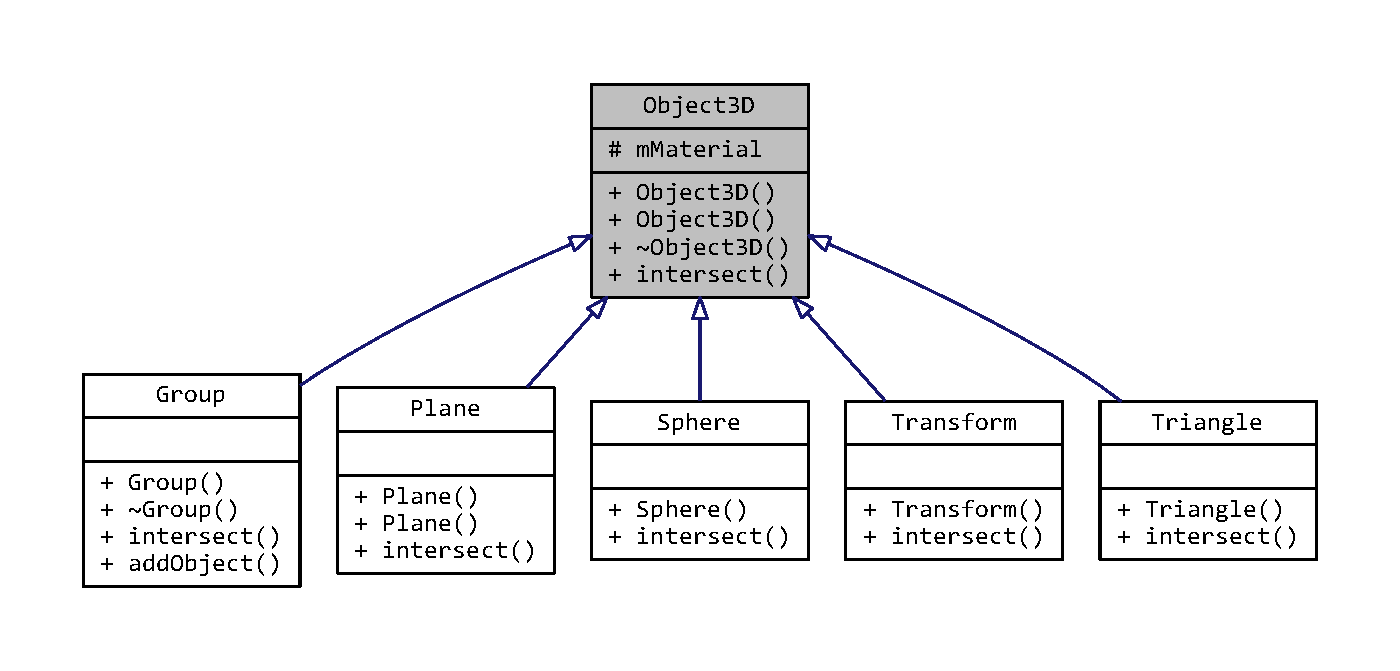
\includegraphics[width=242pt]{classObject3D__inherit__graph}
\end{center}
\end{figure}


\-Collaboration diagram for \-Object3\-D\-:
\nopagebreak
\begin{figure}[H]
\begin{center}
\leavevmode
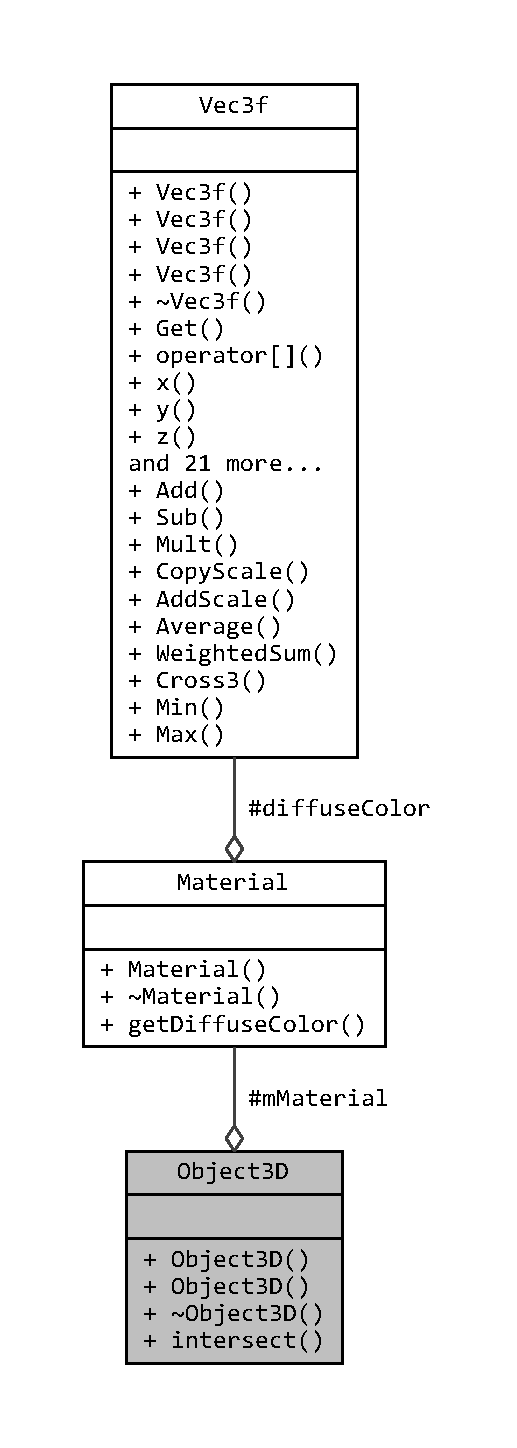
\includegraphics[height=550pt]{classObject3D__coll__graph}
\end{center}
\end{figure}
\subsection*{\-Public \-Member \-Functions}
\begin{DoxyCompactItemize}
\item 
\hypertarget{classObject3D_ae29d1ad924cb8ab4b1b5c5647622f390}{{\bfseries \-Object3\-D} (\hyperlink{classMaterial}{\-Material} $\ast$m)}\label{classObject3D_ae29d1ad924cb8ab4b1b5c5647622f390}

\item 
\hypertarget{classObject3D_a58f07cf2b37c5b6a1c796cd7a939f91b}{virtual bool {\bfseries intersect} (const \hyperlink{classRay}{\-Ray} \&r, \hyperlink{classHit}{\-Hit} \&h, float tmin)=0}\label{classObject3D_a58f07cf2b37c5b6a1c796cd7a939f91b}

\end{DoxyCompactItemize}
\subsection*{\-Protected \-Attributes}
\begin{DoxyCompactItemize}
\item 
\hypertarget{classObject3D_a9eb94e46c928f4f90b1d718119bedaf9}{\hyperlink{classMaterial}{\-Material} $\ast$ {\bfseries m\-Material}}\label{classObject3D_a9eb94e46c928f4f90b1d718119bedaf9}

\end{DoxyCompactItemize}


\-The documentation for this class was generated from the following file\-:\begin{DoxyCompactItemize}
\item 
\-Object3\-D.\-h\end{DoxyCompactItemize}

\hypertarget{classOrthographicCamera}{\section{Orthographic\+Camera Class Reference}
\label{classOrthographicCamera}\index{Orthographic\+Camera@{Orthographic\+Camera}}
}


{\ttfamily \#include $<$Orthographic\+Camera.\+h$>$}



Inheritance diagram for Orthographic\+Camera\+:
\nopagebreak
\begin{figure}[H]
\begin{center}
\leavevmode
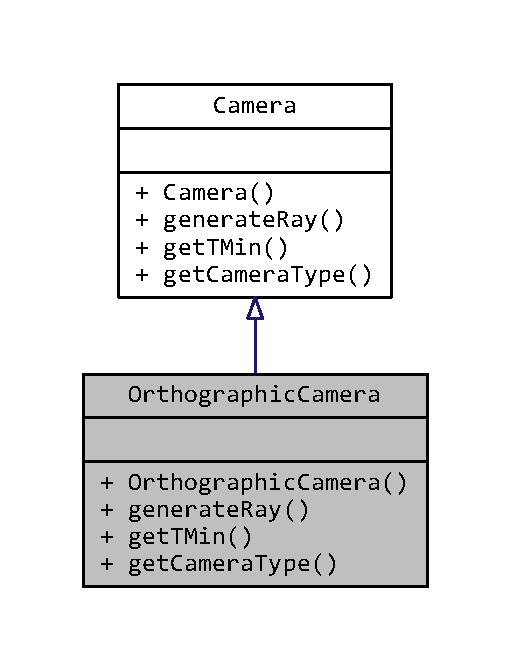
\includegraphics[width=245pt]{classOrthographicCamera__inherit__graph}
\end{center}
\end{figure}


Collaboration diagram for Orthographic\+Camera\+:
\nopagebreak
\begin{figure}[H]
\begin{center}
\leavevmode
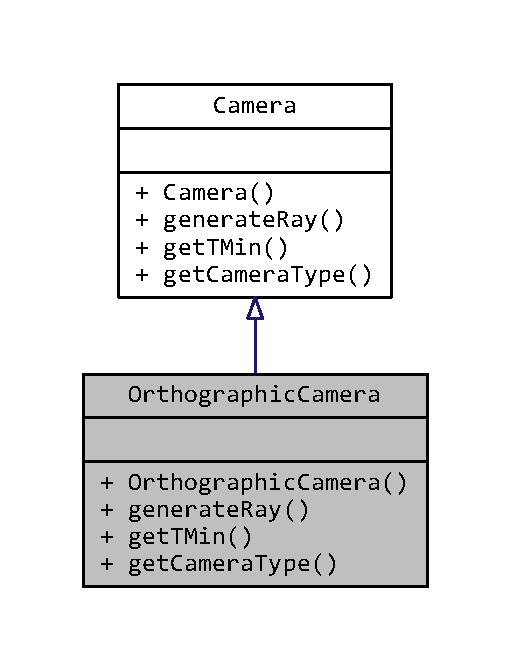
\includegraphics[width=245pt]{classOrthographicCamera__coll__graph}
\end{center}
\end{figure}
\subsection*{Public Member Functions}
\begin{DoxyCompactItemize}
\item 
\hyperlink{classOrthographicCamera_a23c7fec8ea2f52dceee182e4d5d793c6}{Orthographic\+Camera} (const \hyperlink{classVec3f}{Vec3f} \&center, \hyperlink{classVec3f}{Vec3f} \&direction, \hyperlink{classVec3f}{Vec3f} \&up, int size)
\item 
\hyperlink{classRay}{Ray} \hyperlink{classOrthographicCamera_a0d38d086463e985bebc1eeeb8ee1688c}{generate\+Ray} (\hyperlink{classVec2f}{Vec2f} point)
\item 
float \hyperlink{classOrthographicCamera_a8e94c85d863b6e822c6dc41dd6c8c48d}{get\+T\+Min} () const 
\item 
\hyperlink{Camera_8h_af7eb92b45c5f7f64f02821f87c385ebb}{Camera\+Type} \hyperlink{classOrthographicCamera_a971f9b483e42da2a6b8f8026ea6ceec4}{get\+Camera\+Type} ()
\end{DoxyCompactItemize}


\subsection{Constructor \& Destructor Documentation}
\hypertarget{classOrthographicCamera_a23c7fec8ea2f52dceee182e4d5d793c6}{\index{Orthographic\+Camera@{Orthographic\+Camera}!Orthographic\+Camera@{Orthographic\+Camera}}
\index{Orthographic\+Camera@{Orthographic\+Camera}!Orthographic\+Camera@{Orthographic\+Camera}}
\subsubsection[{Orthographic\+Camera}]{\setlength{\rightskip}{0pt plus 5cm}Orthographic\+Camera\+::\+Orthographic\+Camera (
\begin{DoxyParamCaption}
\item[{const {\bf Vec3f} \&}]{center, }
\item[{{\bf Vec3f} \&}]{direction, }
\item[{{\bf Vec3f} \&}]{up, }
\item[{int}]{size}
\end{DoxyParamCaption}
)}}\label{classOrthographicCamera_a23c7fec8ea2f52dceee182e4d5d793c6}


\subsection{Member Function Documentation}
\hypertarget{classOrthographicCamera_a0d38d086463e985bebc1eeeb8ee1688c}{\index{Orthographic\+Camera@{Orthographic\+Camera}!generate\+Ray@{generate\+Ray}}
\index{generate\+Ray@{generate\+Ray}!Orthographic\+Camera@{Orthographic\+Camera}}
\subsubsection[{generate\+Ray}]{\setlength{\rightskip}{0pt plus 5cm}{\bf Ray} Orthographic\+Camera\+::generate\+Ray (
\begin{DoxyParamCaption}
\item[{{\bf Vec2f}}]{point}
\end{DoxyParamCaption}
)\hspace{0.3cm}{\ttfamily [virtual]}}}\label{classOrthographicCamera_a0d38d086463e985bebc1eeeb8ee1688c}


Implements \hyperlink{classCamera_a38dbd2b70b31ee250aadd83b1bbe87fb}{Camera}.

\hypertarget{classOrthographicCamera_a971f9b483e42da2a6b8f8026ea6ceec4}{\index{Orthographic\+Camera@{Orthographic\+Camera}!get\+Camera\+Type@{get\+Camera\+Type}}
\index{get\+Camera\+Type@{get\+Camera\+Type}!Orthographic\+Camera@{Orthographic\+Camera}}
\subsubsection[{get\+Camera\+Type}]{\setlength{\rightskip}{0pt plus 5cm}{\bf Camera\+Type} Orthographic\+Camera\+::get\+Camera\+Type (
\begin{DoxyParamCaption}
{}
\end{DoxyParamCaption}
)\hspace{0.3cm}{\ttfamily [inline]}, {\ttfamily [virtual]}}}\label{classOrthographicCamera_a971f9b483e42da2a6b8f8026ea6ceec4}


Reimplemented from \hyperlink{classCamera_a8ef78e5cc0c5e62077681a0805eb7522}{Camera}.

\hypertarget{classOrthographicCamera_a8e94c85d863b6e822c6dc41dd6c8c48d}{\index{Orthographic\+Camera@{Orthographic\+Camera}!get\+T\+Min@{get\+T\+Min}}
\index{get\+T\+Min@{get\+T\+Min}!Orthographic\+Camera@{Orthographic\+Camera}}
\subsubsection[{get\+T\+Min}]{\setlength{\rightskip}{0pt plus 5cm}float Orthographic\+Camera\+::get\+T\+Min (
\begin{DoxyParamCaption}
{}
\end{DoxyParamCaption}
) const\hspace{0.3cm}{\ttfamily [virtual]}}}\label{classOrthographicCamera_a8e94c85d863b6e822c6dc41dd6c8c48d}


Implements \hyperlink{classCamera_a476000c8588b1aef575482c86153fcb7}{Camera}.



The documentation for this class was generated from the following files\+:\begin{DoxyCompactItemize}
\item 
\hyperlink{OrthographicCamera_8h}{Orthographic\+Camera.\+h}\item 
\hyperlink{OrthographicCamera_8cpp}{Orthographic\+Camera.\+cpp}\end{DoxyCompactItemize}

\hypertarget{classPerspectiveCamera}{\section{Perspective\+Camera Class Reference}
\label{classPerspectiveCamera}\index{Perspective\+Camera@{Perspective\+Camera}}
}


{\ttfamily \#include $<$Perspective\+Camera.\+h$>$}



Inheritance diagram for Perspective\+Camera\+:
\nopagebreak
\begin{figure}[H]
\begin{center}
\leavevmode
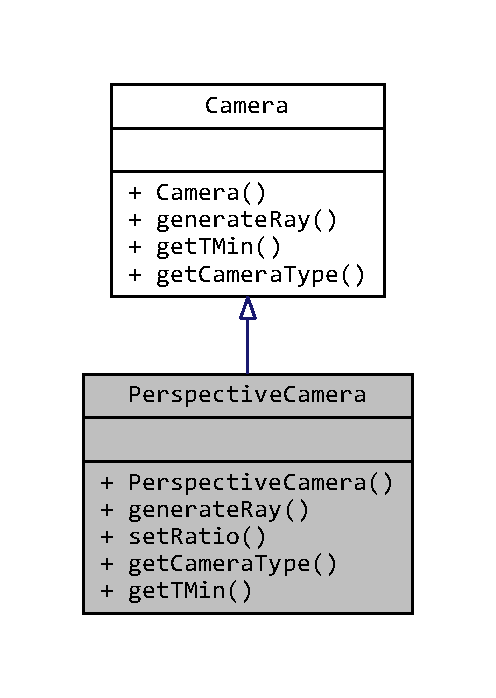
\includegraphics[width=238pt]{classPerspectiveCamera__inherit__graph}
\end{center}
\end{figure}


Collaboration diagram for Perspective\+Camera\+:
\nopagebreak
\begin{figure}[H]
\begin{center}
\leavevmode
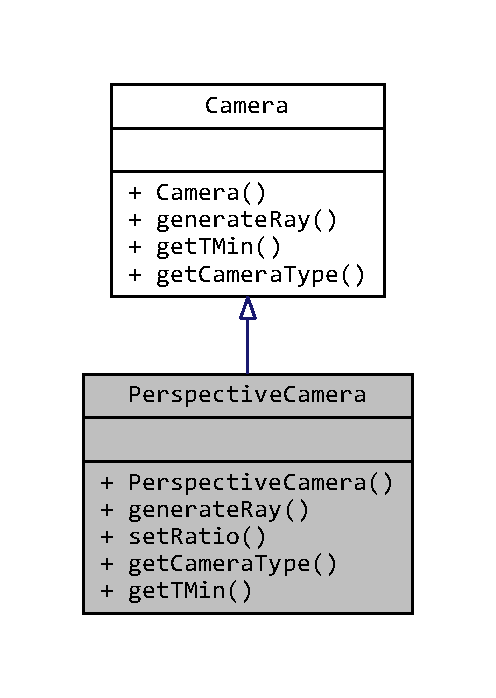
\includegraphics[width=238pt]{classPerspectiveCamera__coll__graph}
\end{center}
\end{figure}
\subsection*{Public Member Functions}
\begin{DoxyCompactItemize}
\item 
\hyperlink{classPerspectiveCamera_a79e25c695b09c9500b585880e726a0f8}{Perspective\+Camera} (\hyperlink{classVec3f}{Vec3f} \&center, \hyperlink{classVec3f}{Vec3f} \&direction, \hyperlink{classVec3f}{Vec3f} \&up, float angle)
\item 
\hyperlink{classRay}{Ray} \hyperlink{classPerspectiveCamera_a28eb145d362d3861f8f92cb25a448602}{generate\+Ray} (\hyperlink{classVec2f}{Vec2f} point)
\item 
void \hyperlink{classPerspectiveCamera_a87c53b9f1c47e4d0c3cf4496fb780f7c}{set\+Ratio} (float ratio)
\item 
\hyperlink{Camera_8h_af7eb92b45c5f7f64f02821f87c385ebb}{Camera\+Type} \hyperlink{classPerspectiveCamera_adc1355f80042153eabbf25f618655655}{get\+Camera\+Type} ()
\item 
float \hyperlink{classPerspectiveCamera_a3a82bc5e9f2fd72faaaf42b3919ecf8a}{get\+T\+Min} () const 
\end{DoxyCompactItemize}


\subsection{Constructor \& Destructor Documentation}
\hypertarget{classPerspectiveCamera_a79e25c695b09c9500b585880e726a0f8}{\index{Perspective\+Camera@{Perspective\+Camera}!Perspective\+Camera@{Perspective\+Camera}}
\index{Perspective\+Camera@{Perspective\+Camera}!Perspective\+Camera@{Perspective\+Camera}}
\subsubsection[{Perspective\+Camera}]{\setlength{\rightskip}{0pt plus 5cm}Perspective\+Camera\+::\+Perspective\+Camera (
\begin{DoxyParamCaption}
\item[{{\bf Vec3f} \&}]{center, }
\item[{{\bf Vec3f} \&}]{direction, }
\item[{{\bf Vec3f} \&}]{up, }
\item[{float}]{angle}
\end{DoxyParamCaption}
)}}\label{classPerspectiveCamera_a79e25c695b09c9500b585880e726a0f8}


\subsection{Member Function Documentation}
\hypertarget{classPerspectiveCamera_a28eb145d362d3861f8f92cb25a448602}{\index{Perspective\+Camera@{Perspective\+Camera}!generate\+Ray@{generate\+Ray}}
\index{generate\+Ray@{generate\+Ray}!Perspective\+Camera@{Perspective\+Camera}}
\subsubsection[{generate\+Ray}]{\setlength{\rightskip}{0pt plus 5cm}{\bf Ray} Perspective\+Camera\+::generate\+Ray (
\begin{DoxyParamCaption}
\item[{{\bf Vec2f}}]{point}
\end{DoxyParamCaption}
)\hspace{0.3cm}{\ttfamily [virtual]}}}\label{classPerspectiveCamera_a28eb145d362d3861f8f92cb25a448602}


Implements \hyperlink{classCamera_a38dbd2b70b31ee250aadd83b1bbe87fb}{Camera}.

\hypertarget{classPerspectiveCamera_adc1355f80042153eabbf25f618655655}{\index{Perspective\+Camera@{Perspective\+Camera}!get\+Camera\+Type@{get\+Camera\+Type}}
\index{get\+Camera\+Type@{get\+Camera\+Type}!Perspective\+Camera@{Perspective\+Camera}}
\subsubsection[{get\+Camera\+Type}]{\setlength{\rightskip}{0pt plus 5cm}{\bf Camera\+Type} Perspective\+Camera\+::get\+Camera\+Type (
\begin{DoxyParamCaption}
{}
\end{DoxyParamCaption}
)\hspace{0.3cm}{\ttfamily [inline]}, {\ttfamily [virtual]}}}\label{classPerspectiveCamera_adc1355f80042153eabbf25f618655655}


Reimplemented from \hyperlink{classCamera_a8ef78e5cc0c5e62077681a0805eb7522}{Camera}.

\hypertarget{classPerspectiveCamera_a3a82bc5e9f2fd72faaaf42b3919ecf8a}{\index{Perspective\+Camera@{Perspective\+Camera}!get\+T\+Min@{get\+T\+Min}}
\index{get\+T\+Min@{get\+T\+Min}!Perspective\+Camera@{Perspective\+Camera}}
\subsubsection[{get\+T\+Min}]{\setlength{\rightskip}{0pt plus 5cm}float Perspective\+Camera\+::get\+T\+Min (
\begin{DoxyParamCaption}
{}
\end{DoxyParamCaption}
) const\hspace{0.3cm}{\ttfamily [inline]}, {\ttfamily [virtual]}}}\label{classPerspectiveCamera_a3a82bc5e9f2fd72faaaf42b3919ecf8a}


Implements \hyperlink{classCamera_a476000c8588b1aef575482c86153fcb7}{Camera}.

\hypertarget{classPerspectiveCamera_a87c53b9f1c47e4d0c3cf4496fb780f7c}{\index{Perspective\+Camera@{Perspective\+Camera}!set\+Ratio@{set\+Ratio}}
\index{set\+Ratio@{set\+Ratio}!Perspective\+Camera@{Perspective\+Camera}}
\subsubsection[{set\+Ratio}]{\setlength{\rightskip}{0pt plus 5cm}void Perspective\+Camera\+::set\+Ratio (
\begin{DoxyParamCaption}
\item[{float}]{ratio}
\end{DoxyParamCaption}
)\hspace{0.3cm}{\ttfamily [inline]}}}\label{classPerspectiveCamera_a87c53b9f1c47e4d0c3cf4496fb780f7c}


The documentation for this class was generated from the following files\+:\begin{DoxyCompactItemize}
\item 
\hyperlink{PerspectiveCamera_8h}{Perspective\+Camera.\+h}\item 
\hyperlink{PerspectiveCamera_8cpp}{Perspective\+Camera.\+cpp}\end{DoxyCompactItemize}

\hypertarget{classPlane}{\section{Plane Class Reference}
\label{classPlane}\index{Plane@{Plane}}
}


{\ttfamily \#include $<$Plane.\+h$>$}



Inheritance diagram for Plane\+:
\nopagebreak
\begin{figure}[H]
\begin{center}
\leavevmode
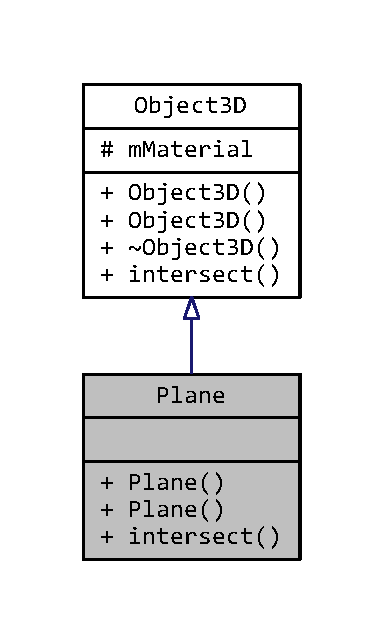
\includegraphics[width=184pt]{classPlane__inherit__graph}
\end{center}
\end{figure}


Collaboration diagram for Plane\+:
\nopagebreak
\begin{figure}[H]
\begin{center}
\leavevmode
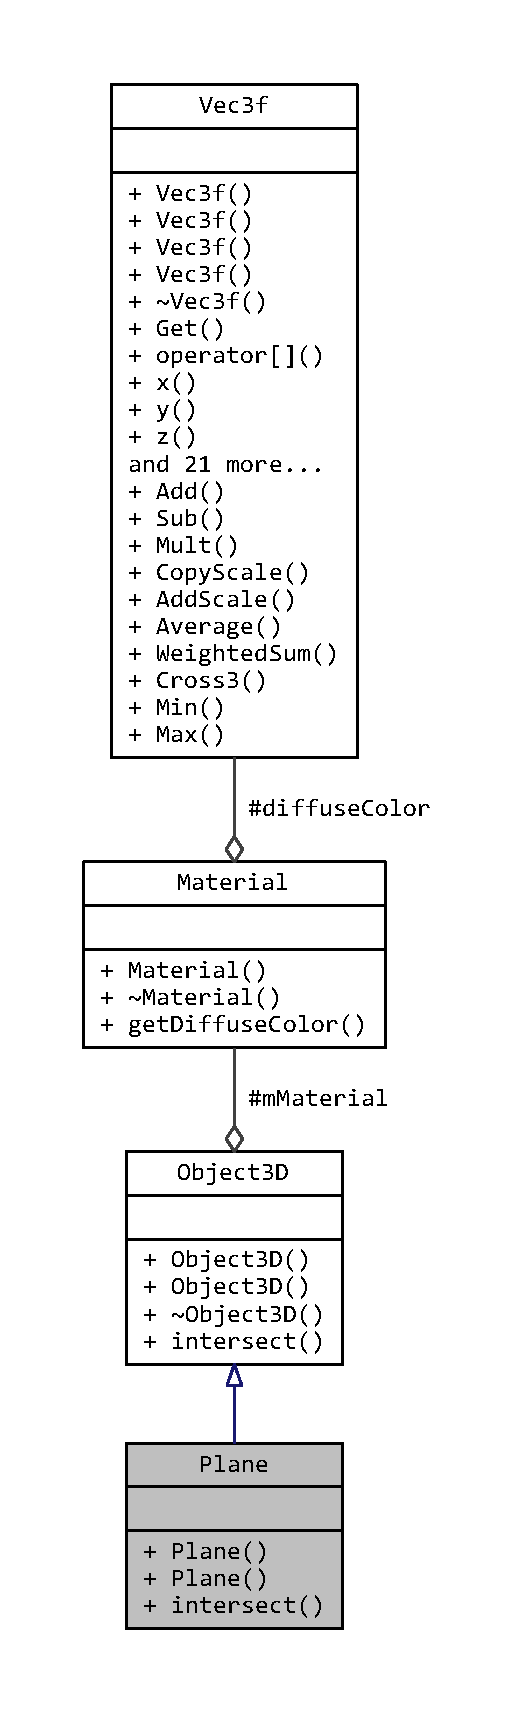
\includegraphics[height=550pt]{classPlane__coll__graph}
\end{center}
\end{figure}
\subsection*{Public Member Functions}
\begin{DoxyCompactItemize}
\item 
\hyperlink{classPlane_a03b8454ad8a2449db6b17f16e5937f30}{Plane} (\hyperlink{classVec3f}{Vec3f} \&normal, float d, \hyperlink{classMaterial}{Material} $\ast$m)
\item 
\hyperlink{classPlane_a615fa23e22e0f4112927ff994a29a015}{Plane} (\hyperlink{classVec3f}{Vec3f} a, \hyperlink{classVec3f}{Vec3f} b, \hyperlink{classVec3f}{Vec3f} c, \hyperlink{classMaterial}{Material} $\ast$m00)
\item 
bool \hyperlink{classPlane_aa5d49b08c1d2bd97f62ede89dccc7298}{intersect} (const \hyperlink{classRay}{Ray} \&r, \hyperlink{classHit}{Hit} \&h, float tmin)
\end{DoxyCompactItemize}
\subsection*{Additional Inherited Members}


\subsection{Constructor \& Destructor Documentation}
\hypertarget{classPlane_a03b8454ad8a2449db6b17f16e5937f30}{\index{Plane@{Plane}!Plane@{Plane}}
\index{Plane@{Plane}!Plane@{Plane}}
\subsubsection[{Plane}]{\setlength{\rightskip}{0pt plus 5cm}Plane\+::\+Plane (
\begin{DoxyParamCaption}
\item[{{\bf Vec3f} \&}]{normal, }
\item[{float}]{d, }
\item[{{\bf Material} $\ast$}]{m}
\end{DoxyParamCaption}
)}}\label{classPlane_a03b8454ad8a2449db6b17f16e5937f30}
\hypertarget{classPlane_a615fa23e22e0f4112927ff994a29a015}{\index{Plane@{Plane}!Plane@{Plane}}
\index{Plane@{Plane}!Plane@{Plane}}
\subsubsection[{Plane}]{\setlength{\rightskip}{0pt plus 5cm}Plane\+::\+Plane (
\begin{DoxyParamCaption}
\item[{{\bf Vec3f}}]{a, }
\item[{{\bf Vec3f}}]{b, }
\item[{{\bf Vec3f}}]{c, }
\item[{{\bf Material} $\ast$}]{m00}
\end{DoxyParamCaption}
)}}\label{classPlane_a615fa23e22e0f4112927ff994a29a015}


\subsection{Member Function Documentation}
\hypertarget{classPlane_aa5d49b08c1d2bd97f62ede89dccc7298}{\index{Plane@{Plane}!intersect@{intersect}}
\index{intersect@{intersect}!Plane@{Plane}}
\subsubsection[{intersect}]{\setlength{\rightskip}{0pt plus 5cm}bool Plane\+::intersect (
\begin{DoxyParamCaption}
\item[{const {\bf Ray} \&}]{r, }
\item[{{\bf Hit} \&}]{h, }
\item[{float}]{tmin}
\end{DoxyParamCaption}
)\hspace{0.3cm}{\ttfamily [virtual]}}}\label{classPlane_aa5d49b08c1d2bd97f62ede89dccc7298}


Implements \hyperlink{classObject3D_a58f07cf2b37c5b6a1c796cd7a939f91b}{Object3\+D}.



The documentation for this class was generated from the following files\+:\begin{DoxyCompactItemize}
\item 
\hyperlink{Plane_8h}{Plane.\+h}\item 
\hyperlink{Plane_8cpp}{Plane.\+cpp}\end{DoxyCompactItemize}

\hypertarget{classRay}{\section{Ray Class Reference}
\label{classRay}\index{Ray@{Ray}}
}


{\ttfamily \#include $<$ray.\+h$>$}



Collaboration diagram for Ray\+:
\nopagebreak
\begin{figure}[H]
\begin{center}
\leavevmode
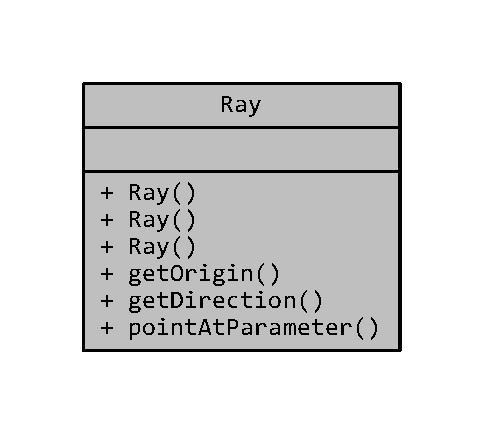
\includegraphics[width=232pt]{classRay__coll__graph}
\end{center}
\end{figure}
\subsection*{Public Member Functions}
\begin{DoxyCompactItemize}
\item 
\hyperlink{classRay_a2e3d2c29f2df4ab3da10da79d4acb852}{Ray} ()
\item 
\hyperlink{classRay_a3f5131016c3a436018e0f37872e887ed}{Ray} (const \hyperlink{classVec3f}{Vec3f} \&orig, const \hyperlink{classVec3f}{Vec3f} \&dir)
\item 
\hyperlink{classRay_a42a3c560d1a0b25412c220025d4f0a94}{Ray} (const \hyperlink{classRay}{Ray} \&r)
\item 
const \hyperlink{classVec3f}{Vec3f} \& \hyperlink{classRay_ad00358184e1d27e1f92ddb10e6d8c5fb}{get\+Origin} () const 
\item 
const \hyperlink{classVec3f}{Vec3f} \& \hyperlink{classRay_a68698a8b94ab05f42ead9f4a89d320f7}{get\+Direction} () const 
\item 
\hyperlink{classVec3f}{Vec3f} \hyperlink{classRay_a3ddbe6537c2fef2c3c638eda9329d66e}{point\+At\+Parameter} (float t) const 
\end{DoxyCompactItemize}


\subsection{Constructor \& Destructor Documentation}
\hypertarget{classRay_a2e3d2c29f2df4ab3da10da79d4acb852}{\index{Ray@{Ray}!Ray@{Ray}}
\index{Ray@{Ray}!Ray@{Ray}}
\subsubsection[{Ray}]{\setlength{\rightskip}{0pt plus 5cm}Ray\+::\+Ray (
\begin{DoxyParamCaption}
{}
\end{DoxyParamCaption}
)\hspace{0.3cm}{\ttfamily [inline]}}}\label{classRay_a2e3d2c29f2df4ab3da10da79d4acb852}
\hypertarget{classRay_a3f5131016c3a436018e0f37872e887ed}{\index{Ray@{Ray}!Ray@{Ray}}
\index{Ray@{Ray}!Ray@{Ray}}
\subsubsection[{Ray}]{\setlength{\rightskip}{0pt plus 5cm}Ray\+::\+Ray (
\begin{DoxyParamCaption}
\item[{const {\bf Vec3f} \&}]{orig, }
\item[{const {\bf Vec3f} \&}]{dir}
\end{DoxyParamCaption}
)\hspace{0.3cm}{\ttfamily [inline]}}}\label{classRay_a3f5131016c3a436018e0f37872e887ed}
\hypertarget{classRay_a42a3c560d1a0b25412c220025d4f0a94}{\index{Ray@{Ray}!Ray@{Ray}}
\index{Ray@{Ray}!Ray@{Ray}}
\subsubsection[{Ray}]{\setlength{\rightskip}{0pt plus 5cm}Ray\+::\+Ray (
\begin{DoxyParamCaption}
\item[{const {\bf Ray} \&}]{r}
\end{DoxyParamCaption}
)\hspace{0.3cm}{\ttfamily [inline]}}}\label{classRay_a42a3c560d1a0b25412c220025d4f0a94}


\subsection{Member Function Documentation}
\hypertarget{classRay_a68698a8b94ab05f42ead9f4a89d320f7}{\index{Ray@{Ray}!get\+Direction@{get\+Direction}}
\index{get\+Direction@{get\+Direction}!Ray@{Ray}}
\subsubsection[{get\+Direction}]{\setlength{\rightskip}{0pt plus 5cm}const {\bf Vec3f}\& Ray\+::get\+Direction (
\begin{DoxyParamCaption}
{}
\end{DoxyParamCaption}
) const\hspace{0.3cm}{\ttfamily [inline]}}}\label{classRay_a68698a8b94ab05f42ead9f4a89d320f7}
\hypertarget{classRay_ad00358184e1d27e1f92ddb10e6d8c5fb}{\index{Ray@{Ray}!get\+Origin@{get\+Origin}}
\index{get\+Origin@{get\+Origin}!Ray@{Ray}}
\subsubsection[{get\+Origin}]{\setlength{\rightskip}{0pt plus 5cm}const {\bf Vec3f}\& Ray\+::get\+Origin (
\begin{DoxyParamCaption}
{}
\end{DoxyParamCaption}
) const\hspace{0.3cm}{\ttfamily [inline]}}}\label{classRay_ad00358184e1d27e1f92ddb10e6d8c5fb}
\hypertarget{classRay_a3ddbe6537c2fef2c3c638eda9329d66e}{\index{Ray@{Ray}!point\+At\+Parameter@{point\+At\+Parameter}}
\index{point\+At\+Parameter@{point\+At\+Parameter}!Ray@{Ray}}
\subsubsection[{point\+At\+Parameter}]{\setlength{\rightskip}{0pt plus 5cm}{\bf Vec3f} Ray\+::point\+At\+Parameter (
\begin{DoxyParamCaption}
\item[{float}]{t}
\end{DoxyParamCaption}
) const\hspace{0.3cm}{\ttfamily [inline]}}}\label{classRay_a3ddbe6537c2fef2c3c638eda9329d66e}


The documentation for this class was generated from the following file\+:\begin{DoxyCompactItemize}
\item 
\hyperlink{ray_8h}{ray.\+h}\end{DoxyCompactItemize}

\hypertarget{classSceneParser}{\section{\-Scene\-Parser \-Class \-Reference}
\label{classSceneParser}\index{\-Scene\-Parser@{\-Scene\-Parser}}
}
\subsection*{\-Public \-Member \-Functions}
\begin{DoxyCompactItemize}
\item 
\hypertarget{classSceneParser_ad88a09b16ec8ebbe49a8fd70e14216cf}{{\bfseries \-Scene\-Parser} (const char $\ast$filename)}\label{classSceneParser_ad88a09b16ec8ebbe49a8fd70e14216cf}

\item 
\hypertarget{classSceneParser_a9fbeeca8f642f40ade54674a41265115}{\hyperlink{classCamera}{\-Camera} $\ast$ {\bfseries get\-Camera} () const }\label{classSceneParser_a9fbeeca8f642f40ade54674a41265115}

\item 
\hypertarget{classSceneParser_a4254064ea79ff601d72d77bc3affb131}{\hyperlink{classVec3f}{\-Vec3f} {\bfseries get\-Background\-Color} () const }\label{classSceneParser_a4254064ea79ff601d72d77bc3affb131}

\item 
\hypertarget{classSceneParser_ae5c6cca64c7bd4f7b9b19c5bb381c801}{int {\bfseries get\-Num\-Materials} () const }\label{classSceneParser_ae5c6cca64c7bd4f7b9b19c5bb381c801}

\item 
\hypertarget{classSceneParser_aadffb5793d5dc58507d20eabb617c6d6}{\hyperlink{classMaterial}{\-Material} $\ast$ {\bfseries get\-Material} (int i) const }\label{classSceneParser_aadffb5793d5dc58507d20eabb617c6d6}

\item 
\hypertarget{classSceneParser_ab7035d29d61e4dfdf64f1e1b4f157b54}{\hyperlink{classGroup}{\-Group} $\ast$ {\bfseries get\-Group} () const }\label{classSceneParser_ab7035d29d61e4dfdf64f1e1b4f157b54}

\end{DoxyCompactItemize}


\-The documentation for this class was generated from the following files\-:\begin{DoxyCompactItemize}
\item 
scene\-\_\-parser.\-h\item 
scene\-\_\-parser.\-cpp\end{DoxyCompactItemize}

\hypertarget{classSphere}{\section{Sphere Class Reference}
\label{classSphere}\index{Sphere@{Sphere}}
}


{\ttfamily \#include $<$Sphere.\+h$>$}



Inheritance diagram for Sphere\+:
\nopagebreak
\begin{figure}[H]
\begin{center}
\leavevmode
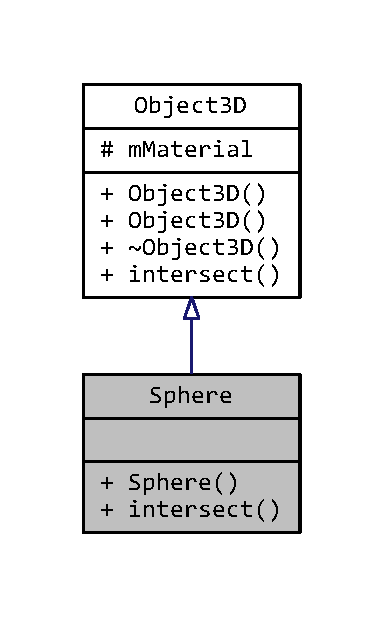
\includegraphics[width=184pt]{classSphere__inherit__graph}
\end{center}
\end{figure}


Collaboration diagram for Sphere\+:
\nopagebreak
\begin{figure}[H]
\begin{center}
\leavevmode
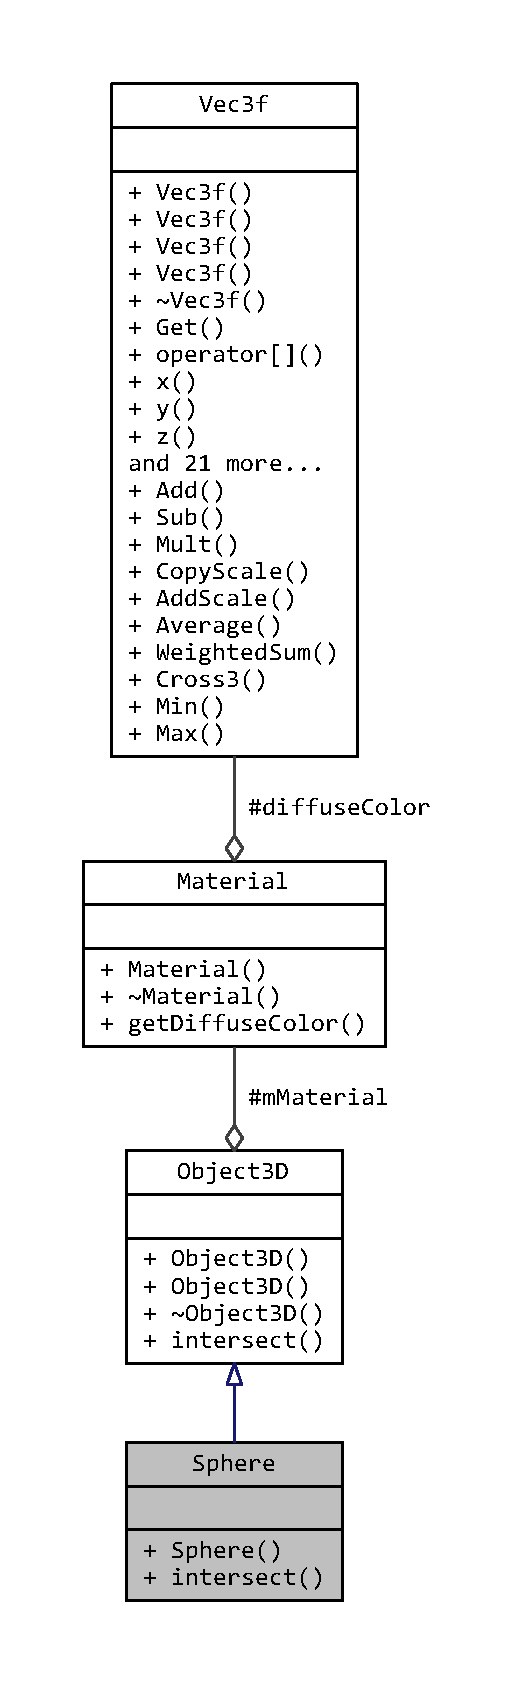
\includegraphics[height=550pt]{classSphere__coll__graph}
\end{center}
\end{figure}
\subsection*{Public Member Functions}
\begin{DoxyCompactItemize}
\item 
\hyperlink{classSphere_aa165eb2886cd16fd67052a2e8e92f6b2}{Sphere} (const \hyperlink{classVec3f}{Vec3f} \&point, float radius, \hyperlink{classMaterial}{Material} $\ast$m)
\item 
bool \hyperlink{classSphere_a87f585d7a2618e8b8974968d4624c92a}{intersect} (const \hyperlink{classRay}{Ray} \&r, \hyperlink{classHit}{Hit} \&h, float tmin)
\end{DoxyCompactItemize}
\subsection*{Additional Inherited Members}


\subsection{Constructor \& Destructor Documentation}
\hypertarget{classSphere_aa165eb2886cd16fd67052a2e8e92f6b2}{\index{Sphere@{Sphere}!Sphere@{Sphere}}
\index{Sphere@{Sphere}!Sphere@{Sphere}}
\subsubsection[{Sphere}]{\setlength{\rightskip}{0pt plus 5cm}Sphere\+::\+Sphere (
\begin{DoxyParamCaption}
\item[{const {\bf Vec3f} \&}]{point, }
\item[{float}]{radius, }
\item[{{\bf Material} $\ast$}]{m}
\end{DoxyParamCaption}
)}}\label{classSphere_aa165eb2886cd16fd67052a2e8e92f6b2}


\subsection{Member Function Documentation}
\hypertarget{classSphere_a87f585d7a2618e8b8974968d4624c92a}{\index{Sphere@{Sphere}!intersect@{intersect}}
\index{intersect@{intersect}!Sphere@{Sphere}}
\subsubsection[{intersect}]{\setlength{\rightskip}{0pt plus 5cm}bool Sphere\+::intersect (
\begin{DoxyParamCaption}
\item[{const {\bf Ray} \&}]{r, }
\item[{{\bf Hit} \&}]{h, }
\item[{float}]{tmin}
\end{DoxyParamCaption}
)\hspace{0.3cm}{\ttfamily [virtual]}}}\label{classSphere_a87f585d7a2618e8b8974968d4624c92a}


Implements \hyperlink{classObject3D_a58f07cf2b37c5b6a1c796cd7a939f91b}{Object3\+D}.



The documentation for this class was generated from the following files\+:\begin{DoxyCompactItemize}
\item 
\hyperlink{Sphere_8h}{Sphere.\+h}\item 
\hyperlink{Sphere_8cpp}{Sphere.\+cpp}\end{DoxyCompactItemize}

\hypertarget{classTransform}{\section{Transform Class Reference}
\label{classTransform}\index{Transform@{Transform}}
}


{\ttfamily \#include $<$Transform.\+h$>$}



Inheritance diagram for Transform\+:
\nopagebreak
\begin{figure}[H]
\begin{center}
\leavevmode
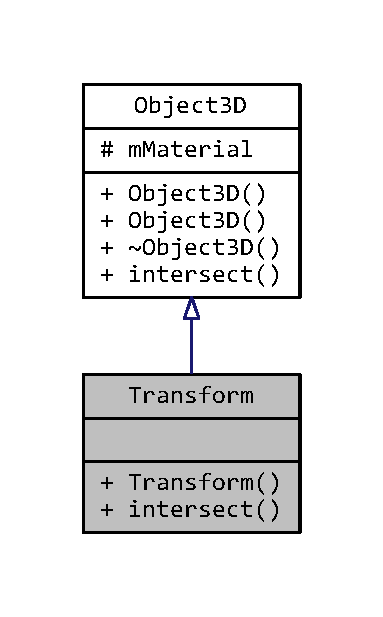
\includegraphics[width=184pt]{classTransform__inherit__graph}
\end{center}
\end{figure}


Collaboration diagram for Transform\+:
\nopagebreak
\begin{figure}[H]
\begin{center}
\leavevmode
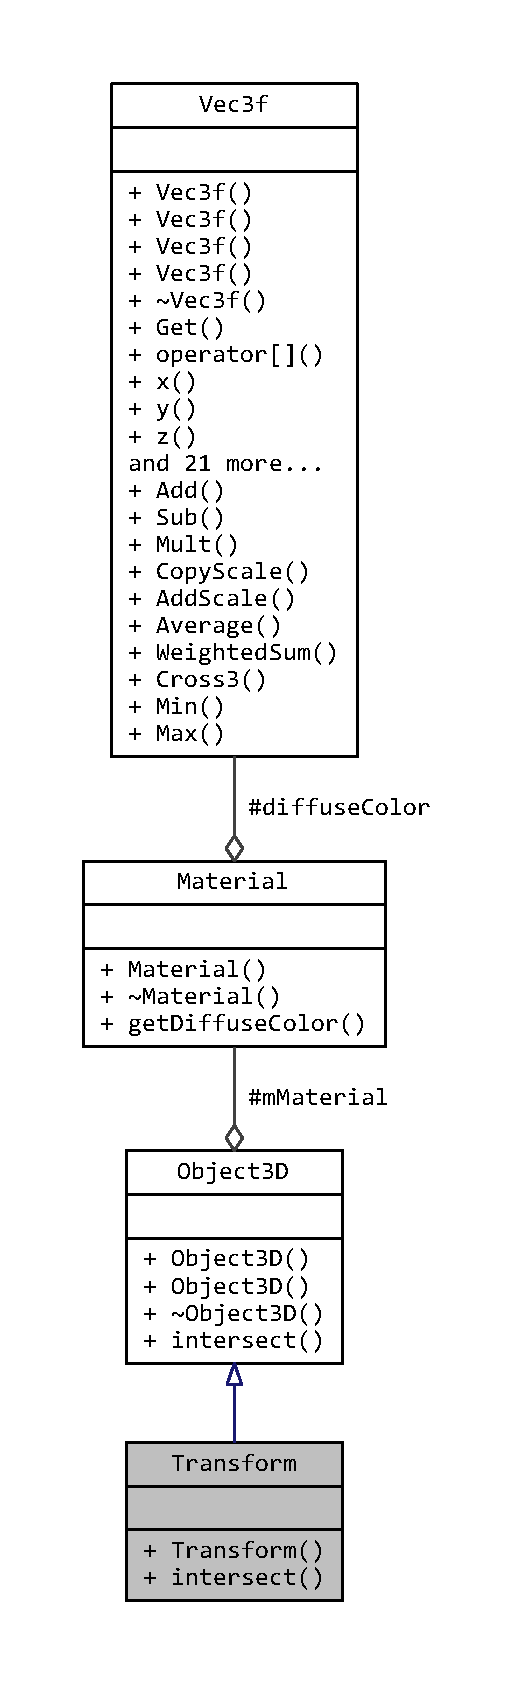
\includegraphics[height=550pt]{classTransform__coll__graph}
\end{center}
\end{figure}
\subsection*{Public Member Functions}
\begin{DoxyCompactItemize}
\item 
\hyperlink{classTransform_aac7b26ca9d450d14e8dbf33ca7cff0aa}{Transform} (\hyperlink{classMatrix}{Matrix} \&m, \hyperlink{classObject3D}{Object3\+D} $\ast$o)
\item 
bool \hyperlink{classTransform_ad91c3a15e08477cc3e78def816d27bd6}{intersect} (const \hyperlink{classRay}{Ray} \&r, \hyperlink{classHit}{Hit} \&h, float tmin)
\end{DoxyCompactItemize}
\subsection*{Additional Inherited Members}


\subsection{Constructor \& Destructor Documentation}
\hypertarget{classTransform_aac7b26ca9d450d14e8dbf33ca7cff0aa}{\index{Transform@{Transform}!Transform@{Transform}}
\index{Transform@{Transform}!Transform@{Transform}}
\subsubsection[{Transform}]{\setlength{\rightskip}{0pt plus 5cm}Transform\+::\+Transform (
\begin{DoxyParamCaption}
\item[{{\bf Matrix} \&}]{m, }
\item[{{\bf Object3\+D} $\ast$}]{o}
\end{DoxyParamCaption}
)}}\label{classTransform_aac7b26ca9d450d14e8dbf33ca7cff0aa}


\subsection{Member Function Documentation}
\hypertarget{classTransform_ad91c3a15e08477cc3e78def816d27bd6}{\index{Transform@{Transform}!intersect@{intersect}}
\index{intersect@{intersect}!Transform@{Transform}}
\subsubsection[{intersect}]{\setlength{\rightskip}{0pt plus 5cm}bool Transform\+::intersect (
\begin{DoxyParamCaption}
\item[{const {\bf Ray} \&}]{r, }
\item[{{\bf Hit} \&}]{h, }
\item[{float}]{tmin}
\end{DoxyParamCaption}
)\hspace{0.3cm}{\ttfamily [virtual]}}}\label{classTransform_ad91c3a15e08477cc3e78def816d27bd6}


Implements \hyperlink{classObject3D_a58f07cf2b37c5b6a1c796cd7a939f91b}{Object3\+D}.



The documentation for this class was generated from the following files\+:\begin{DoxyCompactItemize}
\item 
\hyperlink{Transform_8h}{Transform.\+h}\item 
\hyperlink{Transform_8cpp}{Transform.\+cpp}\end{DoxyCompactItemize}

\hypertarget{classTriangle}{\section{Triangle Class Reference}
\label{classTriangle}\index{Triangle@{Triangle}}
}


{\ttfamily \#include $<$Triangle.\+h$>$}



Inheritance diagram for Triangle\+:
\nopagebreak
\begin{figure}[H]
\begin{center}
\leavevmode
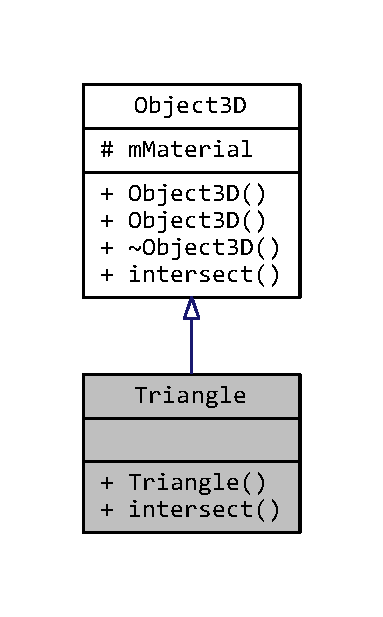
\includegraphics[width=184pt]{classTriangle__inherit__graph}
\end{center}
\end{figure}


Collaboration diagram for Triangle\+:
\nopagebreak
\begin{figure}[H]
\begin{center}
\leavevmode
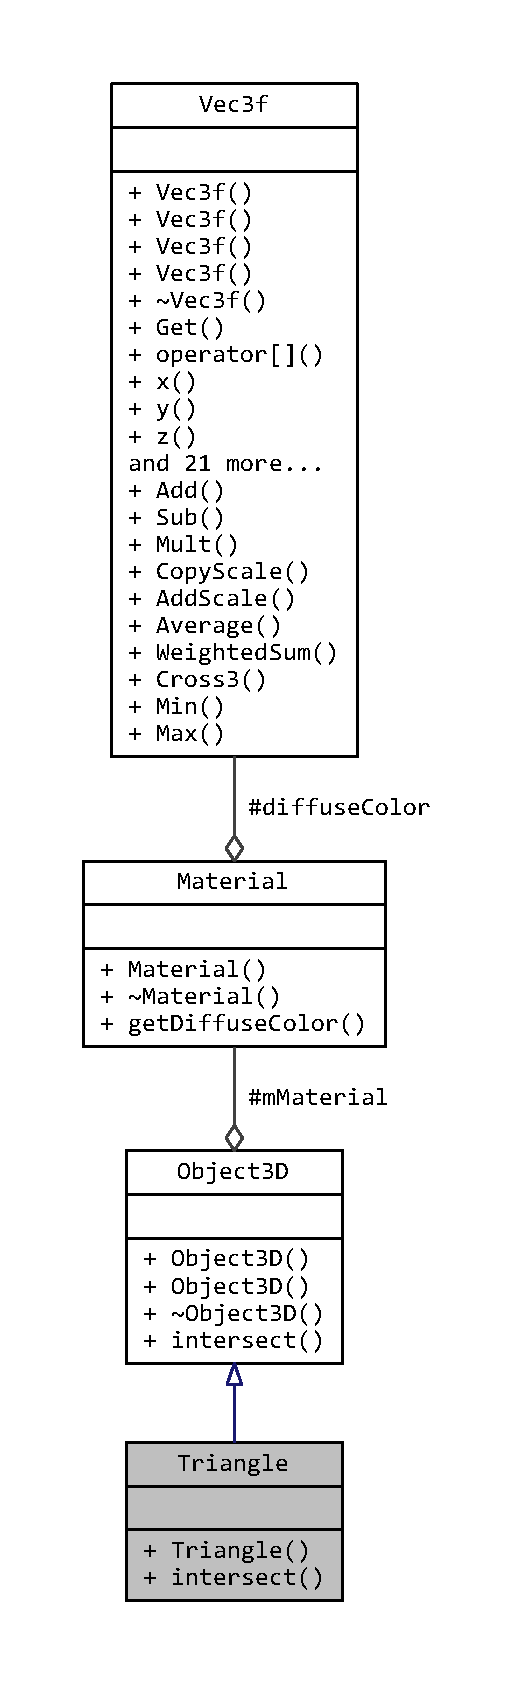
\includegraphics[height=550pt]{classTriangle__coll__graph}
\end{center}
\end{figure}
\subsection*{Public Member Functions}
\begin{DoxyCompactItemize}
\item 
\hyperlink{classTriangle_a47f7f8c2e0fdd8eeb9a0da704f5ccbe4}{Triangle} (\hyperlink{classVec3f}{Vec3f} \&a, \hyperlink{classVec3f}{Vec3f} \&b, \hyperlink{classVec3f}{Vec3f} \&c, \hyperlink{classMaterial}{Material} $\ast$m)
\item 
bool \hyperlink{classTriangle_a3e0979b60f7008812146905eace0f0e5}{intersect} (const \hyperlink{classRay}{Ray} \&r, \hyperlink{classHit}{Hit} \&h, float tmin)
\end{DoxyCompactItemize}
\subsection*{Additional Inherited Members}


\subsection{Constructor \& Destructor Documentation}
\hypertarget{classTriangle_a47f7f8c2e0fdd8eeb9a0da704f5ccbe4}{\index{Triangle@{Triangle}!Triangle@{Triangle}}
\index{Triangle@{Triangle}!Triangle@{Triangle}}
\subsubsection[{Triangle}]{\setlength{\rightskip}{0pt plus 5cm}Triangle\+::\+Triangle (
\begin{DoxyParamCaption}
\item[{{\bf Vec3f} \&}]{a, }
\item[{{\bf Vec3f} \&}]{b, }
\item[{{\bf Vec3f} \&}]{c, }
\item[{{\bf Material} $\ast$}]{m}
\end{DoxyParamCaption}
)}}\label{classTriangle_a47f7f8c2e0fdd8eeb9a0da704f5ccbe4}


\subsection{Member Function Documentation}
\hypertarget{classTriangle_a3e0979b60f7008812146905eace0f0e5}{\index{Triangle@{Triangle}!intersect@{intersect}}
\index{intersect@{intersect}!Triangle@{Triangle}}
\subsubsection[{intersect}]{\setlength{\rightskip}{0pt plus 5cm}bool Triangle\+::intersect (
\begin{DoxyParamCaption}
\item[{const {\bf Ray} \&}]{r, }
\item[{{\bf Hit} \&}]{h, }
\item[{float}]{tmin}
\end{DoxyParamCaption}
)\hspace{0.3cm}{\ttfamily [virtual]}}}\label{classTriangle_a3e0979b60f7008812146905eace0f0e5}


Implements \hyperlink{classObject3D_a58f07cf2b37c5b6a1c796cd7a939f91b}{Object3\+D}.



The documentation for this class was generated from the following files\+:\begin{DoxyCompactItemize}
\item 
\hyperlink{Triangle_8h}{Triangle.\+h}\item 
\hyperlink{Triangle_8cpp}{Triangle.\+cpp}\end{DoxyCompactItemize}

\hypertarget{classVec2f}{\section{Vec2f Class Reference}
\label{classVec2f}\index{Vec2f@{Vec2f}}
}


{\ttfamily \#include $<$vectors.\+h$>$}



Collaboration diagram for Vec2f\+:
\nopagebreak
\begin{figure}[H]
\begin{center}
\leavevmode
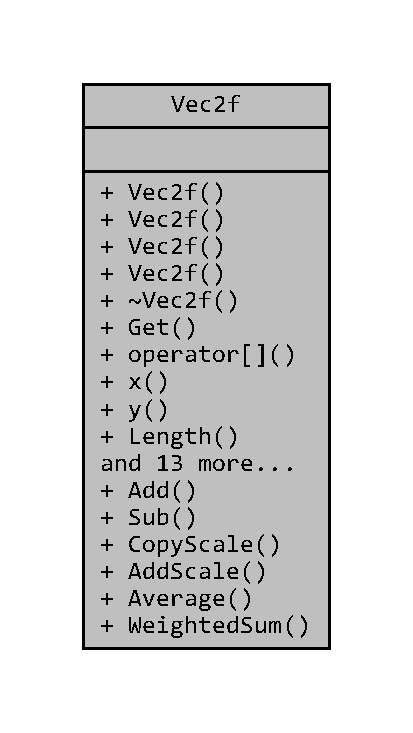
\includegraphics[width=198pt]{classVec2f__coll__graph}
\end{center}
\end{figure}
\subsection*{Public Member Functions}
\begin{DoxyCompactItemize}
\item 
\hyperlink{classVec2f_a3582875fbf3badc6af02646e07bcf440}{Vec2f} ()
\item 
\hyperlink{classVec2f_a1ccd068b35746d18e32a4eace483f6a8}{Vec2f} (const \hyperlink{classVec2f}{Vec2f} \&V)
\item 
\hyperlink{classVec2f_ad05e55e211dd1b8e074f3d7d885702b9}{Vec2f} (float d0, float d1)
\item 
\hyperlink{classVec2f_a3d38f3909d8afebe49d445bce2222f95}{Vec2f} (const \hyperlink{classVec2f}{Vec2f} \&V1, const \hyperlink{classVec2f}{Vec2f} \&V2)
\item 
\hyperlink{classVec2f_a47eb22a462a2c7b7eb61edc07acb94cd}{$\sim$\+Vec2f} ()
\item 
void \hyperlink{classVec2f_a9fae265c16db131c066c14f73612eeeb}{Get} (float \&d0, float \&d1) const 
\item 
float \hyperlink{classVec2f_a289c043da9eeb8b3d2b6431d0e503d7b}{operator\mbox{[}$\,$\mbox{]}} (int i) const 
\item 
float \hyperlink{classVec2f_afa3f111d472b59c28e1d16085672a486}{x} () const 
\item 
float \hyperlink{classVec2f_a95deeb91f6b67910e012afc23e1bee5a}{y} () const 
\item 
float \hyperlink{classVec2f_a4ff073e7f62ee4099033dc000cede267}{Length} () const 
\item 
void \hyperlink{classVec2f_a33fda3509f836bd7edb439dd1704560d}{Set} (float d0, float d1)
\item 
void \hyperlink{classVec2f_a99b9eaccfebc7f10e7931171b1435018}{Scale} (float d0, float d1)
\item 
void \hyperlink{classVec2f_a9e9b6b93359ff9d0dc1208b7ddb37835}{Divide} (float d0, float d1)
\item 
void \hyperlink{classVec2f_a9117c2ca7d92eb0b4cd74916dfd11bf0}{Negate} ()
\item 
\hyperlink{classVec2f}{Vec2f} \& \hyperlink{classVec2f_a09876a9fe3d0e12c16afc31e69d52a95}{operator=} (const \hyperlink{classVec2f}{Vec2f} \&V)
\item 
int \hyperlink{classVec2f_a14005267a1c6a528577ad4d8976a4fd0}{operator==} (const \hyperlink{classVec2f}{Vec2f} \&V) const 
\item 
int \hyperlink{classVec2f_ad35c0e389f6bbcf52b9aabaf0693362f}{operator!=} (const \hyperlink{classVec2f}{Vec2f} \&V)
\item 
\hyperlink{classVec2f}{Vec2f} \& \hyperlink{classVec2f_afcf9b0267e8e4bc489e92536d2a59f94}{operator+=} (const \hyperlink{classVec2f}{Vec2f} \&V)
\item 
\hyperlink{classVec2f}{Vec2f} \& \hyperlink{classVec2f_a7617681b3e723a3e079a7ac9aa1cd5b8}{operator-\/=} (const \hyperlink{classVec2f}{Vec2f} \&V)
\item 
\hyperlink{classVec2f}{Vec2f} \& \hyperlink{classVec2f_a90602c3e9acd18762a488ed2a8393f61}{operator$\ast$=} (float f)
\item 
\hyperlink{classVec2f}{Vec2f} \& \hyperlink{classVec2f_a37cc7be7b91f340669d513e287974eff}{operator/=} (float f)
\item 
float \hyperlink{classVec2f_a827b91f7366c14666cdbb14d471a8aab}{Dot2} (const \hyperlink{classVec2f}{Vec2f} \&V) const 
\item 
void \hyperlink{classVec2f_af423b0af426c519e9301e83f62afe14e}{Write} (F\+I\+L\+E $\ast$F=stdout) const 
\end{DoxyCompactItemize}
\subsection*{Static Public Member Functions}
\begin{DoxyCompactItemize}
\item 
static void \hyperlink{classVec2f_aaa72e50ede2f02d9cbfead98966a6a10}{Add} (\hyperlink{classVec2f}{Vec2f} \&a, const \hyperlink{classVec2f}{Vec2f} \&b, const \hyperlink{classVec2f}{Vec2f} \&c)
\item 
static void \hyperlink{classVec2f_aa3efb59c19587d81ec7ad53ecf12226d}{Sub} (\hyperlink{classVec2f}{Vec2f} \&a, const \hyperlink{classVec2f}{Vec2f} \&b, const \hyperlink{classVec2f}{Vec2f} \&c)
\item 
static void \hyperlink{classVec2f_a32c4b20a2c2b5fae581a4eeae4316c47}{Copy\+Scale} (\hyperlink{classVec2f}{Vec2f} \&a, const \hyperlink{classVec2f}{Vec2f} \&b, float c)
\item 
static void \hyperlink{classVec2f_a80a502fea4f66b921c84019829128ff1}{Add\+Scale} (\hyperlink{classVec2f}{Vec2f} \&a, const \hyperlink{classVec2f}{Vec2f} \&b, const \hyperlink{classVec2f}{Vec2f} \&c, float d)
\item 
static void \hyperlink{classVec2f_ab8bb3386b3363f60cf814fb289528c16}{Average} (\hyperlink{classVec2f}{Vec2f} \&a, const \hyperlink{classVec2f}{Vec2f} \&b, const \hyperlink{classVec2f}{Vec2f} \&c)
\item 
static void \hyperlink{classVec2f_aec7c624674de97ca3cdf2a895d0c1495}{Weighted\+Sum} (\hyperlink{classVec2f}{Vec2f} \&a, const \hyperlink{classVec2f}{Vec2f} \&b, float c, const \hyperlink{classVec2f}{Vec2f} \&d, float e)
\end{DoxyCompactItemize}


\subsection{Constructor \& Destructor Documentation}
\hypertarget{classVec2f_a3582875fbf3badc6af02646e07bcf440}{\index{Vec2f@{Vec2f}!Vec2f@{Vec2f}}
\index{Vec2f@{Vec2f}!Vec2f@{Vec2f}}
\subsubsection[{Vec2f}]{\setlength{\rightskip}{0pt plus 5cm}Vec2f\+::\+Vec2f (
\begin{DoxyParamCaption}
{}
\end{DoxyParamCaption}
)\hspace{0.3cm}{\ttfamily [inline]}}}\label{classVec2f_a3582875fbf3badc6af02646e07bcf440}
\hypertarget{classVec2f_a1ccd068b35746d18e32a4eace483f6a8}{\index{Vec2f@{Vec2f}!Vec2f@{Vec2f}}
\index{Vec2f@{Vec2f}!Vec2f@{Vec2f}}
\subsubsection[{Vec2f}]{\setlength{\rightskip}{0pt plus 5cm}Vec2f\+::\+Vec2f (
\begin{DoxyParamCaption}
\item[{const {\bf Vec2f} \&}]{V}
\end{DoxyParamCaption}
)\hspace{0.3cm}{\ttfamily [inline]}}}\label{classVec2f_a1ccd068b35746d18e32a4eace483f6a8}
\hypertarget{classVec2f_ad05e55e211dd1b8e074f3d7d885702b9}{\index{Vec2f@{Vec2f}!Vec2f@{Vec2f}}
\index{Vec2f@{Vec2f}!Vec2f@{Vec2f}}
\subsubsection[{Vec2f}]{\setlength{\rightskip}{0pt plus 5cm}Vec2f\+::\+Vec2f (
\begin{DoxyParamCaption}
\item[{float}]{d0, }
\item[{float}]{d1}
\end{DoxyParamCaption}
)\hspace{0.3cm}{\ttfamily [inline]}}}\label{classVec2f_ad05e55e211dd1b8e074f3d7d885702b9}
\hypertarget{classVec2f_a3d38f3909d8afebe49d445bce2222f95}{\index{Vec2f@{Vec2f}!Vec2f@{Vec2f}}
\index{Vec2f@{Vec2f}!Vec2f@{Vec2f}}
\subsubsection[{Vec2f}]{\setlength{\rightskip}{0pt plus 5cm}Vec2f\+::\+Vec2f (
\begin{DoxyParamCaption}
\item[{const {\bf Vec2f} \&}]{V1, }
\item[{const {\bf Vec2f} \&}]{V2}
\end{DoxyParamCaption}
)\hspace{0.3cm}{\ttfamily [inline]}}}\label{classVec2f_a3d38f3909d8afebe49d445bce2222f95}
\hypertarget{classVec2f_a47eb22a462a2c7b7eb61edc07acb94cd}{\index{Vec2f@{Vec2f}!````~Vec2f@{$\sim$\+Vec2f}}
\index{````~Vec2f@{$\sim$\+Vec2f}!Vec2f@{Vec2f}}
\subsubsection[{$\sim$\+Vec2f}]{\setlength{\rightskip}{0pt plus 5cm}Vec2f\+::$\sim$\+Vec2f (
\begin{DoxyParamCaption}
{}
\end{DoxyParamCaption}
)\hspace{0.3cm}{\ttfamily [inline]}}}\label{classVec2f_a47eb22a462a2c7b7eb61edc07acb94cd}


\subsection{Member Function Documentation}
\hypertarget{classVec2f_aaa72e50ede2f02d9cbfead98966a6a10}{\index{Vec2f@{Vec2f}!Add@{Add}}
\index{Add@{Add}!Vec2f@{Vec2f}}
\subsubsection[{Add}]{\setlength{\rightskip}{0pt plus 5cm}static void Vec2f\+::\+Add (
\begin{DoxyParamCaption}
\item[{{\bf Vec2f} \&}]{a, }
\item[{const {\bf Vec2f} \&}]{b, }
\item[{const {\bf Vec2f} \&}]{c}
\end{DoxyParamCaption}
)\hspace{0.3cm}{\ttfamily [inline]}, {\ttfamily [static]}}}\label{classVec2f_aaa72e50ede2f02d9cbfead98966a6a10}
\hypertarget{classVec2f_a80a502fea4f66b921c84019829128ff1}{\index{Vec2f@{Vec2f}!Add\+Scale@{Add\+Scale}}
\index{Add\+Scale@{Add\+Scale}!Vec2f@{Vec2f}}
\subsubsection[{Add\+Scale}]{\setlength{\rightskip}{0pt plus 5cm}static void Vec2f\+::\+Add\+Scale (
\begin{DoxyParamCaption}
\item[{{\bf Vec2f} \&}]{a, }
\item[{const {\bf Vec2f} \&}]{b, }
\item[{const {\bf Vec2f} \&}]{c, }
\item[{float}]{d}
\end{DoxyParamCaption}
)\hspace{0.3cm}{\ttfamily [inline]}, {\ttfamily [static]}}}\label{classVec2f_a80a502fea4f66b921c84019829128ff1}
\hypertarget{classVec2f_ab8bb3386b3363f60cf814fb289528c16}{\index{Vec2f@{Vec2f}!Average@{Average}}
\index{Average@{Average}!Vec2f@{Vec2f}}
\subsubsection[{Average}]{\setlength{\rightskip}{0pt plus 5cm}static void Vec2f\+::\+Average (
\begin{DoxyParamCaption}
\item[{{\bf Vec2f} \&}]{a, }
\item[{const {\bf Vec2f} \&}]{b, }
\item[{const {\bf Vec2f} \&}]{c}
\end{DoxyParamCaption}
)\hspace{0.3cm}{\ttfamily [inline]}, {\ttfamily [static]}}}\label{classVec2f_ab8bb3386b3363f60cf814fb289528c16}
\hypertarget{classVec2f_a32c4b20a2c2b5fae581a4eeae4316c47}{\index{Vec2f@{Vec2f}!Copy\+Scale@{Copy\+Scale}}
\index{Copy\+Scale@{Copy\+Scale}!Vec2f@{Vec2f}}
\subsubsection[{Copy\+Scale}]{\setlength{\rightskip}{0pt plus 5cm}static void Vec2f\+::\+Copy\+Scale (
\begin{DoxyParamCaption}
\item[{{\bf Vec2f} \&}]{a, }
\item[{const {\bf Vec2f} \&}]{b, }
\item[{float}]{c}
\end{DoxyParamCaption}
)\hspace{0.3cm}{\ttfamily [inline]}, {\ttfamily [static]}}}\label{classVec2f_a32c4b20a2c2b5fae581a4eeae4316c47}
\hypertarget{classVec2f_a9e9b6b93359ff9d0dc1208b7ddb37835}{\index{Vec2f@{Vec2f}!Divide@{Divide}}
\index{Divide@{Divide}!Vec2f@{Vec2f}}
\subsubsection[{Divide}]{\setlength{\rightskip}{0pt plus 5cm}void Vec2f\+::\+Divide (
\begin{DoxyParamCaption}
\item[{float}]{d0, }
\item[{float}]{d1}
\end{DoxyParamCaption}
)\hspace{0.3cm}{\ttfamily [inline]}}}\label{classVec2f_a9e9b6b93359ff9d0dc1208b7ddb37835}
\hypertarget{classVec2f_a827b91f7366c14666cdbb14d471a8aab}{\index{Vec2f@{Vec2f}!Dot2@{Dot2}}
\index{Dot2@{Dot2}!Vec2f@{Vec2f}}
\subsubsection[{Dot2}]{\setlength{\rightskip}{0pt plus 5cm}float Vec2f\+::\+Dot2 (
\begin{DoxyParamCaption}
\item[{const {\bf Vec2f} \&}]{V}
\end{DoxyParamCaption}
) const\hspace{0.3cm}{\ttfamily [inline]}}}\label{classVec2f_a827b91f7366c14666cdbb14d471a8aab}
\hypertarget{classVec2f_a9fae265c16db131c066c14f73612eeeb}{\index{Vec2f@{Vec2f}!Get@{Get}}
\index{Get@{Get}!Vec2f@{Vec2f}}
\subsubsection[{Get}]{\setlength{\rightskip}{0pt plus 5cm}void Vec2f\+::\+Get (
\begin{DoxyParamCaption}
\item[{float \&}]{d0, }
\item[{float \&}]{d1}
\end{DoxyParamCaption}
) const\hspace{0.3cm}{\ttfamily [inline]}}}\label{classVec2f_a9fae265c16db131c066c14f73612eeeb}
\hypertarget{classVec2f_a4ff073e7f62ee4099033dc000cede267}{\index{Vec2f@{Vec2f}!Length@{Length}}
\index{Length@{Length}!Vec2f@{Vec2f}}
\subsubsection[{Length}]{\setlength{\rightskip}{0pt plus 5cm}float Vec2f\+::\+Length (
\begin{DoxyParamCaption}
{}
\end{DoxyParamCaption}
) const\hspace{0.3cm}{\ttfamily [inline]}}}\label{classVec2f_a4ff073e7f62ee4099033dc000cede267}
\hypertarget{classVec2f_a9117c2ca7d92eb0b4cd74916dfd11bf0}{\index{Vec2f@{Vec2f}!Negate@{Negate}}
\index{Negate@{Negate}!Vec2f@{Vec2f}}
\subsubsection[{Negate}]{\setlength{\rightskip}{0pt plus 5cm}void Vec2f\+::\+Negate (
\begin{DoxyParamCaption}
{}
\end{DoxyParamCaption}
)\hspace{0.3cm}{\ttfamily [inline]}}}\label{classVec2f_a9117c2ca7d92eb0b4cd74916dfd11bf0}
\hypertarget{classVec2f_ad35c0e389f6bbcf52b9aabaf0693362f}{\index{Vec2f@{Vec2f}!operator"!=@{operator"!=}}
\index{operator"!=@{operator"!=}!Vec2f@{Vec2f}}
\subsubsection[{operator"!=}]{\setlength{\rightskip}{0pt plus 5cm}int Vec2f\+::operator!= (
\begin{DoxyParamCaption}
\item[{const {\bf Vec2f} \&}]{V}
\end{DoxyParamCaption}
)\hspace{0.3cm}{\ttfamily [inline]}}}\label{classVec2f_ad35c0e389f6bbcf52b9aabaf0693362f}
\hypertarget{classVec2f_a90602c3e9acd18762a488ed2a8393f61}{\index{Vec2f@{Vec2f}!operator$\ast$=@{operator$\ast$=}}
\index{operator$\ast$=@{operator$\ast$=}!Vec2f@{Vec2f}}
\subsubsection[{operator$\ast$=}]{\setlength{\rightskip}{0pt plus 5cm}{\bf Vec2f}\& Vec2f\+::operator$\ast$= (
\begin{DoxyParamCaption}
\item[{float}]{f}
\end{DoxyParamCaption}
)\hspace{0.3cm}{\ttfamily [inline]}}}\label{classVec2f_a90602c3e9acd18762a488ed2a8393f61}
\hypertarget{classVec2f_afcf9b0267e8e4bc489e92536d2a59f94}{\index{Vec2f@{Vec2f}!operator+=@{operator+=}}
\index{operator+=@{operator+=}!Vec2f@{Vec2f}}
\subsubsection[{operator+=}]{\setlength{\rightskip}{0pt plus 5cm}{\bf Vec2f}\& Vec2f\+::operator+= (
\begin{DoxyParamCaption}
\item[{const {\bf Vec2f} \&}]{V}
\end{DoxyParamCaption}
)\hspace{0.3cm}{\ttfamily [inline]}}}\label{classVec2f_afcf9b0267e8e4bc489e92536d2a59f94}
\hypertarget{classVec2f_a7617681b3e723a3e079a7ac9aa1cd5b8}{\index{Vec2f@{Vec2f}!operator-\/=@{operator-\/=}}
\index{operator-\/=@{operator-\/=}!Vec2f@{Vec2f}}
\subsubsection[{operator-\/=}]{\setlength{\rightskip}{0pt plus 5cm}{\bf Vec2f}\& Vec2f\+::operator-\/= (
\begin{DoxyParamCaption}
\item[{const {\bf Vec2f} \&}]{V}
\end{DoxyParamCaption}
)\hspace{0.3cm}{\ttfamily [inline]}}}\label{classVec2f_a7617681b3e723a3e079a7ac9aa1cd5b8}
\hypertarget{classVec2f_a37cc7be7b91f340669d513e287974eff}{\index{Vec2f@{Vec2f}!operator/=@{operator/=}}
\index{operator/=@{operator/=}!Vec2f@{Vec2f}}
\subsubsection[{operator/=}]{\setlength{\rightskip}{0pt plus 5cm}{\bf Vec2f}\& Vec2f\+::operator/= (
\begin{DoxyParamCaption}
\item[{float}]{f}
\end{DoxyParamCaption}
)\hspace{0.3cm}{\ttfamily [inline]}}}\label{classVec2f_a37cc7be7b91f340669d513e287974eff}
\hypertarget{classVec2f_a09876a9fe3d0e12c16afc31e69d52a95}{\index{Vec2f@{Vec2f}!operator=@{operator=}}
\index{operator=@{operator=}!Vec2f@{Vec2f}}
\subsubsection[{operator=}]{\setlength{\rightskip}{0pt plus 5cm}{\bf Vec2f}\& Vec2f\+::operator= (
\begin{DoxyParamCaption}
\item[{const {\bf Vec2f} \&}]{V}
\end{DoxyParamCaption}
)\hspace{0.3cm}{\ttfamily [inline]}}}\label{classVec2f_a09876a9fe3d0e12c16afc31e69d52a95}
\hypertarget{classVec2f_a14005267a1c6a528577ad4d8976a4fd0}{\index{Vec2f@{Vec2f}!operator==@{operator==}}
\index{operator==@{operator==}!Vec2f@{Vec2f}}
\subsubsection[{operator==}]{\setlength{\rightskip}{0pt plus 5cm}int Vec2f\+::operator== (
\begin{DoxyParamCaption}
\item[{const {\bf Vec2f} \&}]{V}
\end{DoxyParamCaption}
) const\hspace{0.3cm}{\ttfamily [inline]}}}\label{classVec2f_a14005267a1c6a528577ad4d8976a4fd0}
\hypertarget{classVec2f_a289c043da9eeb8b3d2b6431d0e503d7b}{\index{Vec2f@{Vec2f}!operator\mbox{[}$\,$\mbox{]}@{operator[]}}
\index{operator\mbox{[}$\,$\mbox{]}@{operator[]}!Vec2f@{Vec2f}}
\subsubsection[{operator[]}]{\setlength{\rightskip}{0pt plus 5cm}float Vec2f\+::operator\mbox{[}$\,$\mbox{]} (
\begin{DoxyParamCaption}
\item[{int}]{i}
\end{DoxyParamCaption}
) const\hspace{0.3cm}{\ttfamily [inline]}}}\label{classVec2f_a289c043da9eeb8b3d2b6431d0e503d7b}
\hypertarget{classVec2f_a99b9eaccfebc7f10e7931171b1435018}{\index{Vec2f@{Vec2f}!Scale@{Scale}}
\index{Scale@{Scale}!Vec2f@{Vec2f}}
\subsubsection[{Scale}]{\setlength{\rightskip}{0pt plus 5cm}void Vec2f\+::\+Scale (
\begin{DoxyParamCaption}
\item[{float}]{d0, }
\item[{float}]{d1}
\end{DoxyParamCaption}
)\hspace{0.3cm}{\ttfamily [inline]}}}\label{classVec2f_a99b9eaccfebc7f10e7931171b1435018}
\hypertarget{classVec2f_a33fda3509f836bd7edb439dd1704560d}{\index{Vec2f@{Vec2f}!Set@{Set}}
\index{Set@{Set}!Vec2f@{Vec2f}}
\subsubsection[{Set}]{\setlength{\rightskip}{0pt plus 5cm}void Vec2f\+::\+Set (
\begin{DoxyParamCaption}
\item[{float}]{d0, }
\item[{float}]{d1}
\end{DoxyParamCaption}
)\hspace{0.3cm}{\ttfamily [inline]}}}\label{classVec2f_a33fda3509f836bd7edb439dd1704560d}
\hypertarget{classVec2f_aa3efb59c19587d81ec7ad53ecf12226d}{\index{Vec2f@{Vec2f}!Sub@{Sub}}
\index{Sub@{Sub}!Vec2f@{Vec2f}}
\subsubsection[{Sub}]{\setlength{\rightskip}{0pt plus 5cm}static void Vec2f\+::\+Sub (
\begin{DoxyParamCaption}
\item[{{\bf Vec2f} \&}]{a, }
\item[{const {\bf Vec2f} \&}]{b, }
\item[{const {\bf Vec2f} \&}]{c}
\end{DoxyParamCaption}
)\hspace{0.3cm}{\ttfamily [inline]}, {\ttfamily [static]}}}\label{classVec2f_aa3efb59c19587d81ec7ad53ecf12226d}
\hypertarget{classVec2f_aec7c624674de97ca3cdf2a895d0c1495}{\index{Vec2f@{Vec2f}!Weighted\+Sum@{Weighted\+Sum}}
\index{Weighted\+Sum@{Weighted\+Sum}!Vec2f@{Vec2f}}
\subsubsection[{Weighted\+Sum}]{\setlength{\rightskip}{0pt plus 5cm}static void Vec2f\+::\+Weighted\+Sum (
\begin{DoxyParamCaption}
\item[{{\bf Vec2f} \&}]{a, }
\item[{const {\bf Vec2f} \&}]{b, }
\item[{float}]{c, }
\item[{const {\bf Vec2f} \&}]{d, }
\item[{float}]{e}
\end{DoxyParamCaption}
)\hspace{0.3cm}{\ttfamily [inline]}, {\ttfamily [static]}}}\label{classVec2f_aec7c624674de97ca3cdf2a895d0c1495}
\hypertarget{classVec2f_af423b0af426c519e9301e83f62afe14e}{\index{Vec2f@{Vec2f}!Write@{Write}}
\index{Write@{Write}!Vec2f@{Vec2f}}
\subsubsection[{Write}]{\setlength{\rightskip}{0pt plus 5cm}void Vec2f\+::\+Write (
\begin{DoxyParamCaption}
\item[{F\+I\+L\+E $\ast$}]{F = {\ttfamily stdout}}
\end{DoxyParamCaption}
) const\hspace{0.3cm}{\ttfamily [inline]}}}\label{classVec2f_af423b0af426c519e9301e83f62afe14e}
\hypertarget{classVec2f_afa3f111d472b59c28e1d16085672a486}{\index{Vec2f@{Vec2f}!x@{x}}
\index{x@{x}!Vec2f@{Vec2f}}
\subsubsection[{x}]{\setlength{\rightskip}{0pt plus 5cm}float Vec2f\+::x (
\begin{DoxyParamCaption}
{}
\end{DoxyParamCaption}
) const\hspace{0.3cm}{\ttfamily [inline]}}}\label{classVec2f_afa3f111d472b59c28e1d16085672a486}
\hypertarget{classVec2f_a95deeb91f6b67910e012afc23e1bee5a}{\index{Vec2f@{Vec2f}!y@{y}}
\index{y@{y}!Vec2f@{Vec2f}}
\subsubsection[{y}]{\setlength{\rightskip}{0pt plus 5cm}float Vec2f\+::y (
\begin{DoxyParamCaption}
{}
\end{DoxyParamCaption}
) const\hspace{0.3cm}{\ttfamily [inline]}}}\label{classVec2f_a95deeb91f6b67910e012afc23e1bee5a}


The documentation for this class was generated from the following file\+:\begin{DoxyCompactItemize}
\item 
\hyperlink{vectors_8h}{vectors.\+h}\end{DoxyCompactItemize}

\hypertarget{classVec3f}{\section{\-Vec3f \-Class \-Reference}
\label{classVec3f}\index{\-Vec3f@{\-Vec3f}}
}
\subsection*{\-Public \-Member \-Functions}
\begin{DoxyCompactItemize}
\item 
\hypertarget{classVec3f_abcc90a8786e61b9ae87d47f2c3c34acd}{{\bfseries \-Vec3f} (const \hyperlink{classVec3f}{\-Vec3f} \&\-V)}\label{classVec3f_abcc90a8786e61b9ae87d47f2c3c34acd}

\item 
\hypertarget{classVec3f_ad1b720bbc0088455823bfc2816789a2d}{{\bfseries \-Vec3f} (float d0, float d1, float d2)}\label{classVec3f_ad1b720bbc0088455823bfc2816789a2d}

\item 
\hypertarget{classVec3f_a5cddc92d35168ffaf9838fd661ab3d00}{{\bfseries \-Vec3f} (const \hyperlink{classVec3f}{\-Vec3f} \&\-V1, const \hyperlink{classVec3f}{\-Vec3f} \&\-V2)}\label{classVec3f_a5cddc92d35168ffaf9838fd661ab3d00}

\item 
\hypertarget{classVec3f_adc04e55fbdab76f77e2c6b2e3243a489}{void {\bfseries \-Get} (float \&d0, float \&d1, float \&d2) const }\label{classVec3f_adc04e55fbdab76f77e2c6b2e3243a489}

\item 
\hypertarget{classVec3f_a8e50e8a857f6587f04402b9447274e2f}{float {\bfseries operator\mbox{[}$\,$\mbox{]}} (int i) const }\label{classVec3f_a8e50e8a857f6587f04402b9447274e2f}

\item 
\hypertarget{classVec3f_a5c39b153bc4ba10503efbc98932c51d5}{float {\bfseries x} () const }\label{classVec3f_a5c39b153bc4ba10503efbc98932c51d5}

\item 
\hypertarget{classVec3f_a4d9122de39a48f6f18ba4184289b6cc0}{float {\bfseries y} () const }\label{classVec3f_a4d9122de39a48f6f18ba4184289b6cc0}

\item 
\hypertarget{classVec3f_a1e1ebbacd37cdd207a1d4b5dd9f2e80b}{float {\bfseries z} () const }\label{classVec3f_a1e1ebbacd37cdd207a1d4b5dd9f2e80b}

\item 
\hypertarget{classVec3f_aed70ad9eb39c47e2f90435de470d5779}{float {\bfseries r} () const }\label{classVec3f_aed70ad9eb39c47e2f90435de470d5779}

\item 
\hypertarget{classVec3f_ad72c43c133ef70d2ddbc283e6c0a9229}{float {\bfseries g} () const }\label{classVec3f_ad72c43c133ef70d2ddbc283e6c0a9229}

\item 
\hypertarget{classVec3f_a022e6dd724965fa27ba4a448f54a66fe}{float {\bfseries b} () const }\label{classVec3f_a022e6dd724965fa27ba4a448f54a66fe}

\item 
\hypertarget{classVec3f_a4e785c2c10a9d63dc8579c5a00ed60d1}{float {\bfseries \-Length} () const }\label{classVec3f_a4e785c2c10a9d63dc8579c5a00ed60d1}

\item 
\hypertarget{classVec3f_a5271259ed70023efa9109f0ec717f3be}{void {\bfseries \-Set} (float d0, float d1, float d2)}\label{classVec3f_a5271259ed70023efa9109f0ec717f3be}

\item 
\hypertarget{classVec3f_a8a919312d46e28ef591d832e4b7d5896}{void {\bfseries \-Scale} (float d0, float d1, float d2)}\label{classVec3f_a8a919312d46e28ef591d832e4b7d5896}

\item 
\hypertarget{classVec3f_a741c1fcfc370c8f07610fb19bd6e5591}{void {\bfseries \-Divide} (float d0, float d1, float d2)}\label{classVec3f_a741c1fcfc370c8f07610fb19bd6e5591}

\item 
\hypertarget{classVec3f_af0a81998f92a3ec791f88e26dcba04b6}{void {\bfseries \-Normalize} ()}\label{classVec3f_af0a81998f92a3ec791f88e26dcba04b6}

\item 
\hypertarget{classVec3f_a52caf47ad4ce4e87ea8711372f686fcc}{void {\bfseries \-Negate} ()}\label{classVec3f_a52caf47ad4ce4e87ea8711372f686fcc}

\item 
\hypertarget{classVec3f_a6fde73a1fa95ab67c4ba418779ca1a93}{void {\bfseries \-Clamp} (float low=0, float high=1)}\label{classVec3f_a6fde73a1fa95ab67c4ba418779ca1a93}

\item 
\hypertarget{classVec3f_a87fd52c3a87f128e40ef26184f63631e}{\hyperlink{classVec3f}{\-Vec3f} \& {\bfseries operator=} (const \hyperlink{classVec3f}{\-Vec3f} \&\-V)}\label{classVec3f_a87fd52c3a87f128e40ef26184f63631e}

\item 
\hypertarget{classVec3f_a11cf71014645816cbb04a26cf6e05db5}{int {\bfseries operator==} (const \hyperlink{classVec3f}{\-Vec3f} \&\-V)}\label{classVec3f_a11cf71014645816cbb04a26cf6e05db5}

\item 
\hypertarget{classVec3f_a12bfa6655b9b6b903fc826f3a5a99556}{int {\bfseries operator!=} (const \hyperlink{classVec3f}{\-Vec3f} \&\-V)}\label{classVec3f_a12bfa6655b9b6b903fc826f3a5a99556}

\item 
\hypertarget{classVec3f_a012e12e4f4d4185f5850717351e73ebd}{\hyperlink{classVec3f}{\-Vec3f} \& {\bfseries operator+=} (const \hyperlink{classVec3f}{\-Vec3f} \&\-V)}\label{classVec3f_a012e12e4f4d4185f5850717351e73ebd}

\item 
\hypertarget{classVec3f_a052981b67b5c4c54b410246873818297}{\hyperlink{classVec3f}{\-Vec3f} \& {\bfseries operator-\/=} (const \hyperlink{classVec3f}{\-Vec3f} \&\-V)}\label{classVec3f_a052981b67b5c4c54b410246873818297}

\item 
\hypertarget{classVec3f_a8ac720d387f1ab4d3577179f6435133c}{\hyperlink{classVec3f}{\-Vec3f} \& {\bfseries operator$\ast$=} (int i)}\label{classVec3f_a8ac720d387f1ab4d3577179f6435133c}

\item 
\hypertarget{classVec3f_a5647d3c70a29b578010f60bc5cf76cee}{\hyperlink{classVec3f}{\-Vec3f} \& {\bfseries operator$\ast$=} (float f)}\label{classVec3f_a5647d3c70a29b578010f60bc5cf76cee}

\item 
\hypertarget{classVec3f_a5a59d4069dd5d6f353ff5fe75a021e2f}{\hyperlink{classVec3f}{\-Vec3f} \& {\bfseries operator/=} (int i)}\label{classVec3f_a5a59d4069dd5d6f353ff5fe75a021e2f}

\item 
\hypertarget{classVec3f_a47c059393f04ca83ae89a0170df03827}{\hyperlink{classVec3f}{\-Vec3f} \& {\bfseries operator/=} (float f)}\label{classVec3f_a47c059393f04ca83ae89a0170df03827}

\item 
\hypertarget{classVec3f_ad42ff4d372bf88c8ce3e3a73d83f5911}{float {\bfseries \-Dot3} (const \hyperlink{classVec3f}{\-Vec3f} \&\-V) const }\label{classVec3f_ad42ff4d372bf88c8ce3e3a73d83f5911}

\item 
\hypertarget{classVec3f_a245fa514b086b4d9826d41ff4b9e3304}{void {\bfseries \-Write} (\-F\-I\-L\-E $\ast$\-F=stdout) const }\label{classVec3f_a245fa514b086b4d9826d41ff4b9e3304}

\end{DoxyCompactItemize}
\subsection*{\-Static \-Public \-Member \-Functions}
\begin{DoxyCompactItemize}
\item 
\hypertarget{classVec3f_aacdb516f519347a97e3afb4b3eaf85cf}{static void {\bfseries \-Add} (\hyperlink{classVec3f}{\-Vec3f} \&a, const \hyperlink{classVec3f}{\-Vec3f} \&b, const \hyperlink{classVec3f}{\-Vec3f} \&c)}\label{classVec3f_aacdb516f519347a97e3afb4b3eaf85cf}

\item 
\hypertarget{classVec3f_adcc5b655fe33dd68e31ab8c583edb24e}{static void {\bfseries \-Sub} (\hyperlink{classVec3f}{\-Vec3f} \&a, const \hyperlink{classVec3f}{\-Vec3f} \&b, const \hyperlink{classVec3f}{\-Vec3f} \&c)}\label{classVec3f_adcc5b655fe33dd68e31ab8c583edb24e}

\item 
\hypertarget{classVec3f_a47a21f4964e17c407b4eab7b9e9c57ae}{static void {\bfseries \-Mult} (\hyperlink{classVec3f}{\-Vec3f} \&a, const \hyperlink{classVec3f}{\-Vec3f} \&b, const \hyperlink{classVec3f}{\-Vec3f} \&c)}\label{classVec3f_a47a21f4964e17c407b4eab7b9e9c57ae}

\item 
\hypertarget{classVec3f_a0051eb38dab417945be8b3944f17c905}{static void {\bfseries \-Copy\-Scale} (\hyperlink{classVec3f}{\-Vec3f} \&a, const \hyperlink{classVec3f}{\-Vec3f} \&b, float c)}\label{classVec3f_a0051eb38dab417945be8b3944f17c905}

\item 
\hypertarget{classVec3f_aa528c0a3de60ed84203ad55b301b1ac7}{static void {\bfseries \-Add\-Scale} (\hyperlink{classVec3f}{\-Vec3f} \&a, const \hyperlink{classVec3f}{\-Vec3f} \&b, const \hyperlink{classVec3f}{\-Vec3f} \&c, float d)}\label{classVec3f_aa528c0a3de60ed84203ad55b301b1ac7}

\item 
\hypertarget{classVec3f_a8cde49b7f82d31c0a8982481d6ad8135}{static void {\bfseries \-Average} (\hyperlink{classVec3f}{\-Vec3f} \&a, const \hyperlink{classVec3f}{\-Vec3f} \&b, const \hyperlink{classVec3f}{\-Vec3f} \&c)}\label{classVec3f_a8cde49b7f82d31c0a8982481d6ad8135}

\item 
\hypertarget{classVec3f_a57ef802daeae190571da7e5c480d4ccc}{static void {\bfseries \-Weighted\-Sum} (\hyperlink{classVec3f}{\-Vec3f} \&a, const \hyperlink{classVec3f}{\-Vec3f} \&b, float c, const \hyperlink{classVec3f}{\-Vec3f} \&d, float e)}\label{classVec3f_a57ef802daeae190571da7e5c480d4ccc}

\item 
\hypertarget{classVec3f_a07d559fa6f6b5809daeba8ae99051360}{static void {\bfseries \-Cross3} (\hyperlink{classVec3f}{\-Vec3f} \&c, const \hyperlink{classVec3f}{\-Vec3f} \&v1, const \hyperlink{classVec3f}{\-Vec3f} \&v2)}\label{classVec3f_a07d559fa6f6b5809daeba8ae99051360}

\item 
\hypertarget{classVec3f_aa7d7a2d18d4223baa56aab1af7602960}{static void {\bfseries \-Min} (\hyperlink{classVec3f}{\-Vec3f} \&a, const \hyperlink{classVec3f}{\-Vec3f} \&b, const \hyperlink{classVec3f}{\-Vec3f} \&c)}\label{classVec3f_aa7d7a2d18d4223baa56aab1af7602960}

\item 
\hypertarget{classVec3f_a06c5a88aefac724277f118b24df6bd0a}{static void {\bfseries \-Max} (\hyperlink{classVec3f}{\-Vec3f} \&a, const \hyperlink{classVec3f}{\-Vec3f} \&b, const \hyperlink{classVec3f}{\-Vec3f} \&c)}\label{classVec3f_a06c5a88aefac724277f118b24df6bd0a}

\end{DoxyCompactItemize}
\subsection*{\-Friends}
\begin{DoxyCompactItemize}
\item 
\hypertarget{classVec3f_a34913a9261681f734171a6da06bd56fe}{class {\bfseries \-Matrix}}\label{classVec3f_a34913a9261681f734171a6da06bd56fe}

\item 
\hypertarget{classVec3f_a8bb28d98335c4ef8c41a4f031fdc36aa}{\hyperlink{classVec3f}{\-Vec3f} {\bfseries operator+} (const \hyperlink{classVec3f}{\-Vec3f} \&v1, const \hyperlink{classVec3f}{\-Vec3f} \&v2)}\label{classVec3f_a8bb28d98335c4ef8c41a4f031fdc36aa}

\item 
\hypertarget{classVec3f_abcd62ac173dcf5e3e312dbce1fddcd54}{\hyperlink{classVec3f}{\-Vec3f} {\bfseries operator-\/} (const \hyperlink{classVec3f}{\-Vec3f} \&v1, const \hyperlink{classVec3f}{\-Vec3f} \&v2)}\label{classVec3f_abcd62ac173dcf5e3e312dbce1fddcd54}

\item 
\hypertarget{classVec3f_a490eea3a0be4e4978daa382e7fb68845}{\hyperlink{classVec3f}{\-Vec3f} {\bfseries operator$\ast$} (const \hyperlink{classVec3f}{\-Vec3f} \&v1, float f)}\label{classVec3f_a490eea3a0be4e4978daa382e7fb68845}

\item 
\hypertarget{classVec3f_abfe4ec12147bf5ebea8a0cc09da761da}{\hyperlink{classVec3f}{\-Vec3f} {\bfseries operator$\ast$} (float f, const \hyperlink{classVec3f}{\-Vec3f} \&v1)}\label{classVec3f_abfe4ec12147bf5ebea8a0cc09da761da}

\item 
\hypertarget{classVec3f_affeeb0e32bd8c131350b596a89216e35}{\hyperlink{classVec3f}{\-Vec3f} {\bfseries operator$\ast$} (const \hyperlink{classVec3f}{\-Vec3f} \&v1, const \hyperlink{classVec3f}{\-Vec3f} \&v2)}\label{classVec3f_affeeb0e32bd8c131350b596a89216e35}

\end{DoxyCompactItemize}


\-The documentation for this class was generated from the following file\-:\begin{DoxyCompactItemize}
\item 
vectors.\-h\end{DoxyCompactItemize}

\hypertarget{classVec4f}{\section{Vec4f Class Reference}
\label{classVec4f}\index{Vec4f@{Vec4f}}
}


{\ttfamily \#include $<$vectors.\+h$>$}



Collaboration diagram for Vec4f\+:
\nopagebreak
\begin{figure}[H]
\begin{center}
\leavevmode
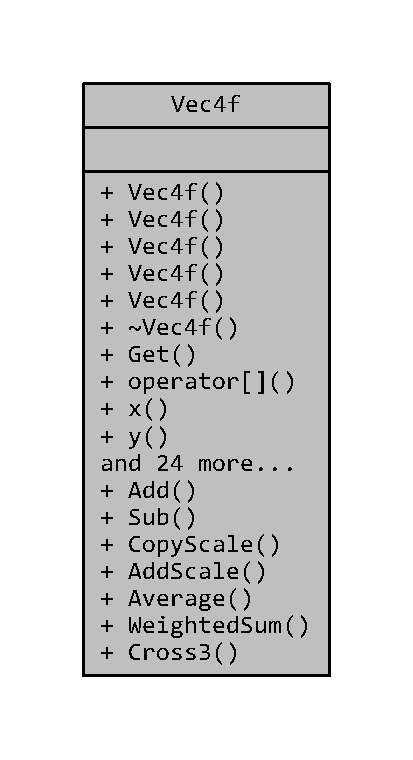
\includegraphics[width=198pt]{classVec4f__coll__graph}
\end{center}
\end{figure}
\subsection*{Public Member Functions}
\begin{DoxyCompactItemize}
\item 
\hyperlink{classVec4f_a5124dad37f3bd310a11bb1592b1456d4}{Vec4f} ()
\item 
\hyperlink{classVec4f_acada261ab1deeff0aecb2b717300cecc}{Vec4f} (const \hyperlink{classVec4f}{Vec4f} \&V)
\item 
\hyperlink{classVec4f_a2d79033898fd342979f9da1f5a318a5a}{Vec4f} (float d0, float d1, float d2, float d3)
\item 
\hyperlink{classVec4f_af93eaed53706e0c147c49846a43cbf5e}{Vec4f} (const \hyperlink{classVec3f}{Vec3f} \&V, float \hyperlink{classVec4f_a50fc37943df263c5c656aa0707b4b5ef}{w})
\item 
\hyperlink{classVec4f_aeb03d44ccc6993f691d4750abcf742a6}{Vec4f} (const \hyperlink{classVec4f}{Vec4f} \&V1, const \hyperlink{classVec4f}{Vec4f} \&V2)
\item 
\hyperlink{classVec4f_a06896138c29aefaa63f86ede0b851f88}{$\sim$\+Vec4f} ()
\item 
void \hyperlink{classVec4f_ac50e2b42ece0ea38319a1da0e35f2901}{Get} (float \&d0, float \&d1, float \&d2, float \&d3) const 
\item 
float \hyperlink{classVec4f_a642f9dd8ba277449ad7e0adc758c75a8}{operator\mbox{[}$\,$\mbox{]}} (int i) const 
\item 
float \hyperlink{classVec4f_a25f2284456fd28a42c0b4e385f968a17}{x} () const 
\item 
float \hyperlink{classVec4f_a2ee69c55784c64a50cc2e0c5eaa974d7}{y} () const 
\item 
float \hyperlink{classVec4f_a810931422b57413fe997648b7b3af01d}{z} () const 
\item 
float \hyperlink{classVec4f_a50fc37943df263c5c656aa0707b4b5ef}{w} () const 
\item 
float \hyperlink{classVec4f_afac8aafe64ff4b5f30c67dd885a912f9}{r} () const 
\item 
float \hyperlink{classVec4f_ac761cb0275da3e8309fa1ea2aa97211f}{g} () const 
\item 
float \hyperlink{classVec4f_a68a0e7c40d2a9a761de53041aad8c577}{b} () const 
\item 
float \hyperlink{classVec4f_af12a900ddc3e3eeb9bbe10d721392f4a}{a} () const 
\item 
float \hyperlink{classVec4f_a374d8d253020a8db79de8a19b0bcfb21}{Length} () const 
\item 
void \hyperlink{classVec4f_aee24f98156cf8f6b7b2c82226c1b45b8}{Set} (float d0, float d1, float d2, float d3)
\item 
void \hyperlink{classVec4f_a4e278a1a03fc75d08b2479434d02a93b}{Scale} (float d0, float d1, float d2, float d3)
\item 
void \hyperlink{classVec4f_a15519ea147364b4f0f4d06f5ed2e84a0}{Divide} (float d0, float d1, float d2, float d3)
\item 
void \hyperlink{classVec4f_afde9b6639cddcd05e50939206070cae5}{Negate} ()
\item 
void \hyperlink{classVec4f_a778c0534a618a205c0e6d270d011a9f4}{Normalize} ()
\item 
void \hyperlink{classVec4f_a73189d23dbecc1961c06890d31eb7eec}{Divide\+By\+W} ()
\item 
\hyperlink{classVec4f}{Vec4f} \& \hyperlink{classVec4f_ad787eea4e2a08a293a21a00adaa52bfa}{operator=} (const \hyperlink{classVec4f}{Vec4f} \&V)
\item 
int \hyperlink{classVec4f_a39e556a72e87d2e7279bb6b743d7ff58}{operator==} (const \hyperlink{classVec4f}{Vec4f} \&V) const 
\item 
int \hyperlink{classVec4f_afd7d07212bb6dcfee2e98a22c163a902}{operator!=} (const \hyperlink{classVec4f}{Vec4f} \&V) const 
\item 
\hyperlink{classVec4f}{Vec4f} \& \hyperlink{classVec4f_a731b923867e74116577d8e6f7aab9b51}{operator+=} (const \hyperlink{classVec4f}{Vec4f} \&V)
\item 
\hyperlink{classVec4f}{Vec4f} \& \hyperlink{classVec4f_abe78d3c5c69e5669ca06c586ec66d59f}{operator-\/=} (const \hyperlink{classVec4f}{Vec4f} \&V)
\item 
\hyperlink{classVec4f}{Vec4f} \& \hyperlink{classVec4f_a13df49c47b3102d318e135839b81ca73}{operator$\ast$=} (float f)
\item 
\hyperlink{classVec4f}{Vec4f} \& \hyperlink{classVec4f_a4319a795f66c8aff5b48e8d3fc6e1bbb}{operator/=} (float f)
\item 
float \hyperlink{classVec4f_a7a3d362d70ab25253051eca6e6d556ae}{Dot2} (const \hyperlink{classVec4f}{Vec4f} \&V) const 
\item 
float \hyperlink{classVec4f_a470fe32036a3b5ed2ad420525fb9ae27}{Dot3} (const \hyperlink{classVec4f}{Vec4f} \&V) const 
\item 
float \hyperlink{classVec4f_a7b235edca512202fc421fed109ac1602}{Dot4} (const \hyperlink{classVec4f}{Vec4f} \&V) const 
\item 
void \hyperlink{classVec4f_a3968afdffe144e4b3e9d81ec8a2bc53c}{Write} (F\+I\+L\+E $\ast$F=stdout) const 
\end{DoxyCompactItemize}
\subsection*{Static Public Member Functions}
\begin{DoxyCompactItemize}
\item 
static void \hyperlink{classVec4f_aff7136abcf44eca7996b108b8906bedd}{Add} (\hyperlink{classVec4f}{Vec4f} \&\hyperlink{classVec4f_af12a900ddc3e3eeb9bbe10d721392f4a}{a}, const \hyperlink{classVec4f}{Vec4f} \&\hyperlink{classVec4f_a68a0e7c40d2a9a761de53041aad8c577}{b}, const \hyperlink{classVec4f}{Vec4f} \&c)
\item 
static void \hyperlink{classVec4f_a21c95b9a1b2f08a4ee48e1f0e7e5c808}{Sub} (\hyperlink{classVec4f}{Vec4f} \&\hyperlink{classVec4f_af12a900ddc3e3eeb9bbe10d721392f4a}{a}, const \hyperlink{classVec4f}{Vec4f} \&\hyperlink{classVec4f_a68a0e7c40d2a9a761de53041aad8c577}{b}, const \hyperlink{classVec4f}{Vec4f} \&c)
\item 
static void \hyperlink{classVec4f_ac0b09b2b5c036d7b941ab45f118762eb}{Copy\+Scale} (\hyperlink{classVec4f}{Vec4f} \&\hyperlink{classVec4f_af12a900ddc3e3eeb9bbe10d721392f4a}{a}, const \hyperlink{classVec4f}{Vec4f} \&\hyperlink{classVec4f_a68a0e7c40d2a9a761de53041aad8c577}{b}, float c)
\item 
static void \hyperlink{classVec4f_a2472e737411650f15535e8326cfea1e7}{Add\+Scale} (\hyperlink{classVec4f}{Vec4f} \&\hyperlink{classVec4f_af12a900ddc3e3eeb9bbe10d721392f4a}{a}, const \hyperlink{classVec4f}{Vec4f} \&\hyperlink{classVec4f_a68a0e7c40d2a9a761de53041aad8c577}{b}, const \hyperlink{classVec4f}{Vec4f} \&c, float d)
\item 
static void \hyperlink{classVec4f_a64205b1fc41a26f522d90f6f19413bc7}{Average} (\hyperlink{classVec4f}{Vec4f} \&\hyperlink{classVec4f_af12a900ddc3e3eeb9bbe10d721392f4a}{a}, const \hyperlink{classVec4f}{Vec4f} \&\hyperlink{classVec4f_a68a0e7c40d2a9a761de53041aad8c577}{b}, const \hyperlink{classVec4f}{Vec4f} \&c)
\item 
static void \hyperlink{classVec4f_a0ebe3a270ffec1f678b49807df1ae492}{Weighted\+Sum} (\hyperlink{classVec4f}{Vec4f} \&\hyperlink{classVec4f_af12a900ddc3e3eeb9bbe10d721392f4a}{a}, const \hyperlink{classVec4f}{Vec4f} \&\hyperlink{classVec4f_a68a0e7c40d2a9a761de53041aad8c577}{b}, float c, const \hyperlink{classVec4f}{Vec4f} \&d, float e)
\item 
static void \hyperlink{classVec4f_a89dc15455e6e5373dbae79d1c8b0adff}{Cross3} (\hyperlink{classVec4f}{Vec4f} \&c, const \hyperlink{classVec4f}{Vec4f} \&v1, const \hyperlink{classVec4f}{Vec4f} \&v2)
\end{DoxyCompactItemize}
\subsection*{Friends}
\begin{DoxyCompactItemize}
\item 
class \hyperlink{classVec4f_a34913a9261681f734171a6da06bd56fe}{Matrix}
\end{DoxyCompactItemize}


\subsection{Constructor \& Destructor Documentation}
\hypertarget{classVec4f_a5124dad37f3bd310a11bb1592b1456d4}{\index{Vec4f@{Vec4f}!Vec4f@{Vec4f}}
\index{Vec4f@{Vec4f}!Vec4f@{Vec4f}}
\subsubsection[{Vec4f}]{\setlength{\rightskip}{0pt plus 5cm}Vec4f\+::\+Vec4f (
\begin{DoxyParamCaption}
{}
\end{DoxyParamCaption}
)\hspace{0.3cm}{\ttfamily [inline]}}}\label{classVec4f_a5124dad37f3bd310a11bb1592b1456d4}
\hypertarget{classVec4f_acada261ab1deeff0aecb2b717300cecc}{\index{Vec4f@{Vec4f}!Vec4f@{Vec4f}}
\index{Vec4f@{Vec4f}!Vec4f@{Vec4f}}
\subsubsection[{Vec4f}]{\setlength{\rightskip}{0pt plus 5cm}Vec4f\+::\+Vec4f (
\begin{DoxyParamCaption}
\item[{const {\bf Vec4f} \&}]{V}
\end{DoxyParamCaption}
)\hspace{0.3cm}{\ttfamily [inline]}}}\label{classVec4f_acada261ab1deeff0aecb2b717300cecc}
\hypertarget{classVec4f_a2d79033898fd342979f9da1f5a318a5a}{\index{Vec4f@{Vec4f}!Vec4f@{Vec4f}}
\index{Vec4f@{Vec4f}!Vec4f@{Vec4f}}
\subsubsection[{Vec4f}]{\setlength{\rightskip}{0pt plus 5cm}Vec4f\+::\+Vec4f (
\begin{DoxyParamCaption}
\item[{float}]{d0, }
\item[{float}]{d1, }
\item[{float}]{d2, }
\item[{float}]{d3}
\end{DoxyParamCaption}
)\hspace{0.3cm}{\ttfamily [inline]}}}\label{classVec4f_a2d79033898fd342979f9da1f5a318a5a}
\hypertarget{classVec4f_af93eaed53706e0c147c49846a43cbf5e}{\index{Vec4f@{Vec4f}!Vec4f@{Vec4f}}
\index{Vec4f@{Vec4f}!Vec4f@{Vec4f}}
\subsubsection[{Vec4f}]{\setlength{\rightskip}{0pt plus 5cm}Vec4f\+::\+Vec4f (
\begin{DoxyParamCaption}
\item[{const {\bf Vec3f} \&}]{V, }
\item[{float}]{w}
\end{DoxyParamCaption}
)\hspace{0.3cm}{\ttfamily [inline]}}}\label{classVec4f_af93eaed53706e0c147c49846a43cbf5e}
\hypertarget{classVec4f_aeb03d44ccc6993f691d4750abcf742a6}{\index{Vec4f@{Vec4f}!Vec4f@{Vec4f}}
\index{Vec4f@{Vec4f}!Vec4f@{Vec4f}}
\subsubsection[{Vec4f}]{\setlength{\rightskip}{0pt plus 5cm}Vec4f\+::\+Vec4f (
\begin{DoxyParamCaption}
\item[{const {\bf Vec4f} \&}]{V1, }
\item[{const {\bf Vec4f} \&}]{V2}
\end{DoxyParamCaption}
)\hspace{0.3cm}{\ttfamily [inline]}}}\label{classVec4f_aeb03d44ccc6993f691d4750abcf742a6}
\hypertarget{classVec4f_a06896138c29aefaa63f86ede0b851f88}{\index{Vec4f@{Vec4f}!````~Vec4f@{$\sim$\+Vec4f}}
\index{````~Vec4f@{$\sim$\+Vec4f}!Vec4f@{Vec4f}}
\subsubsection[{$\sim$\+Vec4f}]{\setlength{\rightskip}{0pt plus 5cm}Vec4f\+::$\sim$\+Vec4f (
\begin{DoxyParamCaption}
{}
\end{DoxyParamCaption}
)\hspace{0.3cm}{\ttfamily [inline]}}}\label{classVec4f_a06896138c29aefaa63f86ede0b851f88}


\subsection{Member Function Documentation}
\hypertarget{classVec4f_af12a900ddc3e3eeb9bbe10d721392f4a}{\index{Vec4f@{Vec4f}!a@{a}}
\index{a@{a}!Vec4f@{Vec4f}}
\subsubsection[{a}]{\setlength{\rightskip}{0pt plus 5cm}float Vec4f\+::a (
\begin{DoxyParamCaption}
{}
\end{DoxyParamCaption}
) const\hspace{0.3cm}{\ttfamily [inline]}}}\label{classVec4f_af12a900ddc3e3eeb9bbe10d721392f4a}
\hypertarget{classVec4f_aff7136abcf44eca7996b108b8906bedd}{\index{Vec4f@{Vec4f}!Add@{Add}}
\index{Add@{Add}!Vec4f@{Vec4f}}
\subsubsection[{Add}]{\setlength{\rightskip}{0pt plus 5cm}static void Vec4f\+::\+Add (
\begin{DoxyParamCaption}
\item[{{\bf Vec4f} \&}]{a, }
\item[{const {\bf Vec4f} \&}]{b, }
\item[{const {\bf Vec4f} \&}]{c}
\end{DoxyParamCaption}
)\hspace{0.3cm}{\ttfamily [inline]}, {\ttfamily [static]}}}\label{classVec4f_aff7136abcf44eca7996b108b8906bedd}
\hypertarget{classVec4f_a2472e737411650f15535e8326cfea1e7}{\index{Vec4f@{Vec4f}!Add\+Scale@{Add\+Scale}}
\index{Add\+Scale@{Add\+Scale}!Vec4f@{Vec4f}}
\subsubsection[{Add\+Scale}]{\setlength{\rightskip}{0pt plus 5cm}static void Vec4f\+::\+Add\+Scale (
\begin{DoxyParamCaption}
\item[{{\bf Vec4f} \&}]{a, }
\item[{const {\bf Vec4f} \&}]{b, }
\item[{const {\bf Vec4f} \&}]{c, }
\item[{float}]{d}
\end{DoxyParamCaption}
)\hspace{0.3cm}{\ttfamily [inline]}, {\ttfamily [static]}}}\label{classVec4f_a2472e737411650f15535e8326cfea1e7}
\hypertarget{classVec4f_a64205b1fc41a26f522d90f6f19413bc7}{\index{Vec4f@{Vec4f}!Average@{Average}}
\index{Average@{Average}!Vec4f@{Vec4f}}
\subsubsection[{Average}]{\setlength{\rightskip}{0pt plus 5cm}static void Vec4f\+::\+Average (
\begin{DoxyParamCaption}
\item[{{\bf Vec4f} \&}]{a, }
\item[{const {\bf Vec4f} \&}]{b, }
\item[{const {\bf Vec4f} \&}]{c}
\end{DoxyParamCaption}
)\hspace{0.3cm}{\ttfamily [inline]}, {\ttfamily [static]}}}\label{classVec4f_a64205b1fc41a26f522d90f6f19413bc7}
\hypertarget{classVec4f_a68a0e7c40d2a9a761de53041aad8c577}{\index{Vec4f@{Vec4f}!b@{b}}
\index{b@{b}!Vec4f@{Vec4f}}
\subsubsection[{b}]{\setlength{\rightskip}{0pt plus 5cm}float Vec4f\+::b (
\begin{DoxyParamCaption}
{}
\end{DoxyParamCaption}
) const\hspace{0.3cm}{\ttfamily [inline]}}}\label{classVec4f_a68a0e7c40d2a9a761de53041aad8c577}
\hypertarget{classVec4f_ac0b09b2b5c036d7b941ab45f118762eb}{\index{Vec4f@{Vec4f}!Copy\+Scale@{Copy\+Scale}}
\index{Copy\+Scale@{Copy\+Scale}!Vec4f@{Vec4f}}
\subsubsection[{Copy\+Scale}]{\setlength{\rightskip}{0pt plus 5cm}static void Vec4f\+::\+Copy\+Scale (
\begin{DoxyParamCaption}
\item[{{\bf Vec4f} \&}]{a, }
\item[{const {\bf Vec4f} \&}]{b, }
\item[{float}]{c}
\end{DoxyParamCaption}
)\hspace{0.3cm}{\ttfamily [inline]}, {\ttfamily [static]}}}\label{classVec4f_ac0b09b2b5c036d7b941ab45f118762eb}
\hypertarget{classVec4f_a89dc15455e6e5373dbae79d1c8b0adff}{\index{Vec4f@{Vec4f}!Cross3@{Cross3}}
\index{Cross3@{Cross3}!Vec4f@{Vec4f}}
\subsubsection[{Cross3}]{\setlength{\rightskip}{0pt plus 5cm}static void Vec4f\+::\+Cross3 (
\begin{DoxyParamCaption}
\item[{{\bf Vec4f} \&}]{c, }
\item[{const {\bf Vec4f} \&}]{v1, }
\item[{const {\bf Vec4f} \&}]{v2}
\end{DoxyParamCaption}
)\hspace{0.3cm}{\ttfamily [inline]}, {\ttfamily [static]}}}\label{classVec4f_a89dc15455e6e5373dbae79d1c8b0adff}
\hypertarget{classVec4f_a15519ea147364b4f0f4d06f5ed2e84a0}{\index{Vec4f@{Vec4f}!Divide@{Divide}}
\index{Divide@{Divide}!Vec4f@{Vec4f}}
\subsubsection[{Divide}]{\setlength{\rightskip}{0pt plus 5cm}void Vec4f\+::\+Divide (
\begin{DoxyParamCaption}
\item[{float}]{d0, }
\item[{float}]{d1, }
\item[{float}]{d2, }
\item[{float}]{d3}
\end{DoxyParamCaption}
)\hspace{0.3cm}{\ttfamily [inline]}}}\label{classVec4f_a15519ea147364b4f0f4d06f5ed2e84a0}
\hypertarget{classVec4f_a73189d23dbecc1961c06890d31eb7eec}{\index{Vec4f@{Vec4f}!Divide\+By\+W@{Divide\+By\+W}}
\index{Divide\+By\+W@{Divide\+By\+W}!Vec4f@{Vec4f}}
\subsubsection[{Divide\+By\+W}]{\setlength{\rightskip}{0pt plus 5cm}void Vec4f\+::\+Divide\+By\+W (
\begin{DoxyParamCaption}
{}
\end{DoxyParamCaption}
)\hspace{0.3cm}{\ttfamily [inline]}}}\label{classVec4f_a73189d23dbecc1961c06890d31eb7eec}
\hypertarget{classVec4f_a7a3d362d70ab25253051eca6e6d556ae}{\index{Vec4f@{Vec4f}!Dot2@{Dot2}}
\index{Dot2@{Dot2}!Vec4f@{Vec4f}}
\subsubsection[{Dot2}]{\setlength{\rightskip}{0pt plus 5cm}float Vec4f\+::\+Dot2 (
\begin{DoxyParamCaption}
\item[{const {\bf Vec4f} \&}]{V}
\end{DoxyParamCaption}
) const\hspace{0.3cm}{\ttfamily [inline]}}}\label{classVec4f_a7a3d362d70ab25253051eca6e6d556ae}
\hypertarget{classVec4f_a470fe32036a3b5ed2ad420525fb9ae27}{\index{Vec4f@{Vec4f}!Dot3@{Dot3}}
\index{Dot3@{Dot3}!Vec4f@{Vec4f}}
\subsubsection[{Dot3}]{\setlength{\rightskip}{0pt plus 5cm}float Vec4f\+::\+Dot3 (
\begin{DoxyParamCaption}
\item[{const {\bf Vec4f} \&}]{V}
\end{DoxyParamCaption}
) const\hspace{0.3cm}{\ttfamily [inline]}}}\label{classVec4f_a470fe32036a3b5ed2ad420525fb9ae27}
\hypertarget{classVec4f_a7b235edca512202fc421fed109ac1602}{\index{Vec4f@{Vec4f}!Dot4@{Dot4}}
\index{Dot4@{Dot4}!Vec4f@{Vec4f}}
\subsubsection[{Dot4}]{\setlength{\rightskip}{0pt plus 5cm}float Vec4f\+::\+Dot4 (
\begin{DoxyParamCaption}
\item[{const {\bf Vec4f} \&}]{V}
\end{DoxyParamCaption}
) const\hspace{0.3cm}{\ttfamily [inline]}}}\label{classVec4f_a7b235edca512202fc421fed109ac1602}
\hypertarget{classVec4f_ac761cb0275da3e8309fa1ea2aa97211f}{\index{Vec4f@{Vec4f}!g@{g}}
\index{g@{g}!Vec4f@{Vec4f}}
\subsubsection[{g}]{\setlength{\rightskip}{0pt plus 5cm}float Vec4f\+::g (
\begin{DoxyParamCaption}
{}
\end{DoxyParamCaption}
) const\hspace{0.3cm}{\ttfamily [inline]}}}\label{classVec4f_ac761cb0275da3e8309fa1ea2aa97211f}
\hypertarget{classVec4f_ac50e2b42ece0ea38319a1da0e35f2901}{\index{Vec4f@{Vec4f}!Get@{Get}}
\index{Get@{Get}!Vec4f@{Vec4f}}
\subsubsection[{Get}]{\setlength{\rightskip}{0pt plus 5cm}void Vec4f\+::\+Get (
\begin{DoxyParamCaption}
\item[{float \&}]{d0, }
\item[{float \&}]{d1, }
\item[{float \&}]{d2, }
\item[{float \&}]{d3}
\end{DoxyParamCaption}
) const\hspace{0.3cm}{\ttfamily [inline]}}}\label{classVec4f_ac50e2b42ece0ea38319a1da0e35f2901}
\hypertarget{classVec4f_a374d8d253020a8db79de8a19b0bcfb21}{\index{Vec4f@{Vec4f}!Length@{Length}}
\index{Length@{Length}!Vec4f@{Vec4f}}
\subsubsection[{Length}]{\setlength{\rightskip}{0pt plus 5cm}float Vec4f\+::\+Length (
\begin{DoxyParamCaption}
{}
\end{DoxyParamCaption}
) const\hspace{0.3cm}{\ttfamily [inline]}}}\label{classVec4f_a374d8d253020a8db79de8a19b0bcfb21}
\hypertarget{classVec4f_afde9b6639cddcd05e50939206070cae5}{\index{Vec4f@{Vec4f}!Negate@{Negate}}
\index{Negate@{Negate}!Vec4f@{Vec4f}}
\subsubsection[{Negate}]{\setlength{\rightskip}{0pt plus 5cm}void Vec4f\+::\+Negate (
\begin{DoxyParamCaption}
{}
\end{DoxyParamCaption}
)\hspace{0.3cm}{\ttfamily [inline]}}}\label{classVec4f_afde9b6639cddcd05e50939206070cae5}
\hypertarget{classVec4f_a778c0534a618a205c0e6d270d011a9f4}{\index{Vec4f@{Vec4f}!Normalize@{Normalize}}
\index{Normalize@{Normalize}!Vec4f@{Vec4f}}
\subsubsection[{Normalize}]{\setlength{\rightskip}{0pt plus 5cm}void Vec4f\+::\+Normalize (
\begin{DoxyParamCaption}
{}
\end{DoxyParamCaption}
)\hspace{0.3cm}{\ttfamily [inline]}}}\label{classVec4f_a778c0534a618a205c0e6d270d011a9f4}
\hypertarget{classVec4f_afd7d07212bb6dcfee2e98a22c163a902}{\index{Vec4f@{Vec4f}!operator"!=@{operator"!=}}
\index{operator"!=@{operator"!=}!Vec4f@{Vec4f}}
\subsubsection[{operator"!=}]{\setlength{\rightskip}{0pt plus 5cm}int Vec4f\+::operator!= (
\begin{DoxyParamCaption}
\item[{const {\bf Vec4f} \&}]{V}
\end{DoxyParamCaption}
) const\hspace{0.3cm}{\ttfamily [inline]}}}\label{classVec4f_afd7d07212bb6dcfee2e98a22c163a902}
\hypertarget{classVec4f_a13df49c47b3102d318e135839b81ca73}{\index{Vec4f@{Vec4f}!operator$\ast$=@{operator$\ast$=}}
\index{operator$\ast$=@{operator$\ast$=}!Vec4f@{Vec4f}}
\subsubsection[{operator$\ast$=}]{\setlength{\rightskip}{0pt plus 5cm}{\bf Vec4f}\& Vec4f\+::operator$\ast$= (
\begin{DoxyParamCaption}
\item[{float}]{f}
\end{DoxyParamCaption}
)\hspace{0.3cm}{\ttfamily [inline]}}}\label{classVec4f_a13df49c47b3102d318e135839b81ca73}
\hypertarget{classVec4f_a731b923867e74116577d8e6f7aab9b51}{\index{Vec4f@{Vec4f}!operator+=@{operator+=}}
\index{operator+=@{operator+=}!Vec4f@{Vec4f}}
\subsubsection[{operator+=}]{\setlength{\rightskip}{0pt plus 5cm}{\bf Vec4f}\& Vec4f\+::operator+= (
\begin{DoxyParamCaption}
\item[{const {\bf Vec4f} \&}]{V}
\end{DoxyParamCaption}
)\hspace{0.3cm}{\ttfamily [inline]}}}\label{classVec4f_a731b923867e74116577d8e6f7aab9b51}
\hypertarget{classVec4f_abe78d3c5c69e5669ca06c586ec66d59f}{\index{Vec4f@{Vec4f}!operator-\/=@{operator-\/=}}
\index{operator-\/=@{operator-\/=}!Vec4f@{Vec4f}}
\subsubsection[{operator-\/=}]{\setlength{\rightskip}{0pt plus 5cm}{\bf Vec4f}\& Vec4f\+::operator-\/= (
\begin{DoxyParamCaption}
\item[{const {\bf Vec4f} \&}]{V}
\end{DoxyParamCaption}
)\hspace{0.3cm}{\ttfamily [inline]}}}\label{classVec4f_abe78d3c5c69e5669ca06c586ec66d59f}
\hypertarget{classVec4f_a4319a795f66c8aff5b48e8d3fc6e1bbb}{\index{Vec4f@{Vec4f}!operator/=@{operator/=}}
\index{operator/=@{operator/=}!Vec4f@{Vec4f}}
\subsubsection[{operator/=}]{\setlength{\rightskip}{0pt plus 5cm}{\bf Vec4f}\& Vec4f\+::operator/= (
\begin{DoxyParamCaption}
\item[{float}]{f}
\end{DoxyParamCaption}
)\hspace{0.3cm}{\ttfamily [inline]}}}\label{classVec4f_a4319a795f66c8aff5b48e8d3fc6e1bbb}
\hypertarget{classVec4f_ad787eea4e2a08a293a21a00adaa52bfa}{\index{Vec4f@{Vec4f}!operator=@{operator=}}
\index{operator=@{operator=}!Vec4f@{Vec4f}}
\subsubsection[{operator=}]{\setlength{\rightskip}{0pt plus 5cm}{\bf Vec4f}\& Vec4f\+::operator= (
\begin{DoxyParamCaption}
\item[{const {\bf Vec4f} \&}]{V}
\end{DoxyParamCaption}
)\hspace{0.3cm}{\ttfamily [inline]}}}\label{classVec4f_ad787eea4e2a08a293a21a00adaa52bfa}
\hypertarget{classVec4f_a39e556a72e87d2e7279bb6b743d7ff58}{\index{Vec4f@{Vec4f}!operator==@{operator==}}
\index{operator==@{operator==}!Vec4f@{Vec4f}}
\subsubsection[{operator==}]{\setlength{\rightskip}{0pt plus 5cm}int Vec4f\+::operator== (
\begin{DoxyParamCaption}
\item[{const {\bf Vec4f} \&}]{V}
\end{DoxyParamCaption}
) const\hspace{0.3cm}{\ttfamily [inline]}}}\label{classVec4f_a39e556a72e87d2e7279bb6b743d7ff58}
\hypertarget{classVec4f_a642f9dd8ba277449ad7e0adc758c75a8}{\index{Vec4f@{Vec4f}!operator\mbox{[}$\,$\mbox{]}@{operator[]}}
\index{operator\mbox{[}$\,$\mbox{]}@{operator[]}!Vec4f@{Vec4f}}
\subsubsection[{operator[]}]{\setlength{\rightskip}{0pt plus 5cm}float Vec4f\+::operator\mbox{[}$\,$\mbox{]} (
\begin{DoxyParamCaption}
\item[{int}]{i}
\end{DoxyParamCaption}
) const\hspace{0.3cm}{\ttfamily [inline]}}}\label{classVec4f_a642f9dd8ba277449ad7e0adc758c75a8}
\hypertarget{classVec4f_afac8aafe64ff4b5f30c67dd885a912f9}{\index{Vec4f@{Vec4f}!r@{r}}
\index{r@{r}!Vec4f@{Vec4f}}
\subsubsection[{r}]{\setlength{\rightskip}{0pt plus 5cm}float Vec4f\+::r (
\begin{DoxyParamCaption}
{}
\end{DoxyParamCaption}
) const\hspace{0.3cm}{\ttfamily [inline]}}}\label{classVec4f_afac8aafe64ff4b5f30c67dd885a912f9}
\hypertarget{classVec4f_a4e278a1a03fc75d08b2479434d02a93b}{\index{Vec4f@{Vec4f}!Scale@{Scale}}
\index{Scale@{Scale}!Vec4f@{Vec4f}}
\subsubsection[{Scale}]{\setlength{\rightskip}{0pt plus 5cm}void Vec4f\+::\+Scale (
\begin{DoxyParamCaption}
\item[{float}]{d0, }
\item[{float}]{d1, }
\item[{float}]{d2, }
\item[{float}]{d3}
\end{DoxyParamCaption}
)\hspace{0.3cm}{\ttfamily [inline]}}}\label{classVec4f_a4e278a1a03fc75d08b2479434d02a93b}
\hypertarget{classVec4f_aee24f98156cf8f6b7b2c82226c1b45b8}{\index{Vec4f@{Vec4f}!Set@{Set}}
\index{Set@{Set}!Vec4f@{Vec4f}}
\subsubsection[{Set}]{\setlength{\rightskip}{0pt plus 5cm}void Vec4f\+::\+Set (
\begin{DoxyParamCaption}
\item[{float}]{d0, }
\item[{float}]{d1, }
\item[{float}]{d2, }
\item[{float}]{d3}
\end{DoxyParamCaption}
)\hspace{0.3cm}{\ttfamily [inline]}}}\label{classVec4f_aee24f98156cf8f6b7b2c82226c1b45b8}
\hypertarget{classVec4f_a21c95b9a1b2f08a4ee48e1f0e7e5c808}{\index{Vec4f@{Vec4f}!Sub@{Sub}}
\index{Sub@{Sub}!Vec4f@{Vec4f}}
\subsubsection[{Sub}]{\setlength{\rightskip}{0pt plus 5cm}static void Vec4f\+::\+Sub (
\begin{DoxyParamCaption}
\item[{{\bf Vec4f} \&}]{a, }
\item[{const {\bf Vec4f} \&}]{b, }
\item[{const {\bf Vec4f} \&}]{c}
\end{DoxyParamCaption}
)\hspace{0.3cm}{\ttfamily [inline]}, {\ttfamily [static]}}}\label{classVec4f_a21c95b9a1b2f08a4ee48e1f0e7e5c808}
\hypertarget{classVec4f_a50fc37943df263c5c656aa0707b4b5ef}{\index{Vec4f@{Vec4f}!w@{w}}
\index{w@{w}!Vec4f@{Vec4f}}
\subsubsection[{w}]{\setlength{\rightskip}{0pt plus 5cm}float Vec4f\+::w (
\begin{DoxyParamCaption}
{}
\end{DoxyParamCaption}
) const\hspace{0.3cm}{\ttfamily [inline]}}}\label{classVec4f_a50fc37943df263c5c656aa0707b4b5ef}
\hypertarget{classVec4f_a0ebe3a270ffec1f678b49807df1ae492}{\index{Vec4f@{Vec4f}!Weighted\+Sum@{Weighted\+Sum}}
\index{Weighted\+Sum@{Weighted\+Sum}!Vec4f@{Vec4f}}
\subsubsection[{Weighted\+Sum}]{\setlength{\rightskip}{0pt plus 5cm}static void Vec4f\+::\+Weighted\+Sum (
\begin{DoxyParamCaption}
\item[{{\bf Vec4f} \&}]{a, }
\item[{const {\bf Vec4f} \&}]{b, }
\item[{float}]{c, }
\item[{const {\bf Vec4f} \&}]{d, }
\item[{float}]{e}
\end{DoxyParamCaption}
)\hspace{0.3cm}{\ttfamily [inline]}, {\ttfamily [static]}}}\label{classVec4f_a0ebe3a270ffec1f678b49807df1ae492}
\hypertarget{classVec4f_a3968afdffe144e4b3e9d81ec8a2bc53c}{\index{Vec4f@{Vec4f}!Write@{Write}}
\index{Write@{Write}!Vec4f@{Vec4f}}
\subsubsection[{Write}]{\setlength{\rightskip}{0pt plus 5cm}void Vec4f\+::\+Write (
\begin{DoxyParamCaption}
\item[{F\+I\+L\+E $\ast$}]{F = {\ttfamily stdout}}
\end{DoxyParamCaption}
) const\hspace{0.3cm}{\ttfamily [inline]}}}\label{classVec4f_a3968afdffe144e4b3e9d81ec8a2bc53c}
\hypertarget{classVec4f_a25f2284456fd28a42c0b4e385f968a17}{\index{Vec4f@{Vec4f}!x@{x}}
\index{x@{x}!Vec4f@{Vec4f}}
\subsubsection[{x}]{\setlength{\rightskip}{0pt plus 5cm}float Vec4f\+::x (
\begin{DoxyParamCaption}
{}
\end{DoxyParamCaption}
) const\hspace{0.3cm}{\ttfamily [inline]}}}\label{classVec4f_a25f2284456fd28a42c0b4e385f968a17}
\hypertarget{classVec4f_a2ee69c55784c64a50cc2e0c5eaa974d7}{\index{Vec4f@{Vec4f}!y@{y}}
\index{y@{y}!Vec4f@{Vec4f}}
\subsubsection[{y}]{\setlength{\rightskip}{0pt plus 5cm}float Vec4f\+::y (
\begin{DoxyParamCaption}
{}
\end{DoxyParamCaption}
) const\hspace{0.3cm}{\ttfamily [inline]}}}\label{classVec4f_a2ee69c55784c64a50cc2e0c5eaa974d7}
\hypertarget{classVec4f_a810931422b57413fe997648b7b3af01d}{\index{Vec4f@{Vec4f}!z@{z}}
\index{z@{z}!Vec4f@{Vec4f}}
\subsubsection[{z}]{\setlength{\rightskip}{0pt plus 5cm}float Vec4f\+::z (
\begin{DoxyParamCaption}
{}
\end{DoxyParamCaption}
) const\hspace{0.3cm}{\ttfamily [inline]}}}\label{classVec4f_a810931422b57413fe997648b7b3af01d}


\subsection{Friends And Related Function Documentation}
\hypertarget{classVec4f_a34913a9261681f734171a6da06bd56fe}{\index{Vec4f@{Vec4f}!Matrix@{Matrix}}
\index{Matrix@{Matrix}!Vec4f@{Vec4f}}
\subsubsection[{Matrix}]{\setlength{\rightskip}{0pt plus 5cm}friend class {\bf Matrix}\hspace{0.3cm}{\ttfamily [friend]}}}\label{classVec4f_a34913a9261681f734171a6da06bd56fe}


The documentation for this class was generated from the following file\+:\begin{DoxyCompactItemize}
\item 
\hyperlink{vectors_8h}{vectors.\+h}\end{DoxyCompactItemize}

\chapter{File Documentation}
\hypertarget{Camera_8h}{\section{Camera.\+h File Reference}
\label{Camera_8h}\index{Camera.\+h@{Camera.\+h}}
}
{\ttfamily \#include \char`\"{}vectors.\+h\char`\"{}}\\*
{\ttfamily \#include \char`\"{}ray.\+h\char`\"{}}\\*
Include dependency graph for Camera.\+h\+:
\nopagebreak
\begin{figure}[H]
\begin{center}
\leavevmode
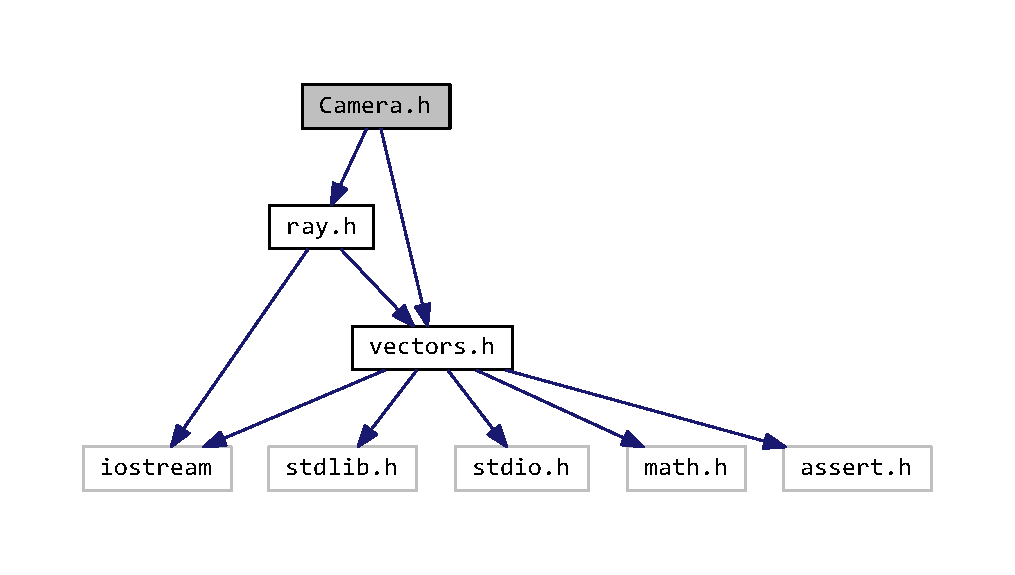
\includegraphics[width=350pt]{Camera_8h__incl}
\end{center}
\end{figure}
This graph shows which files directly or indirectly include this file\+:
\nopagebreak
\begin{figure}[H]
\begin{center}
\leavevmode
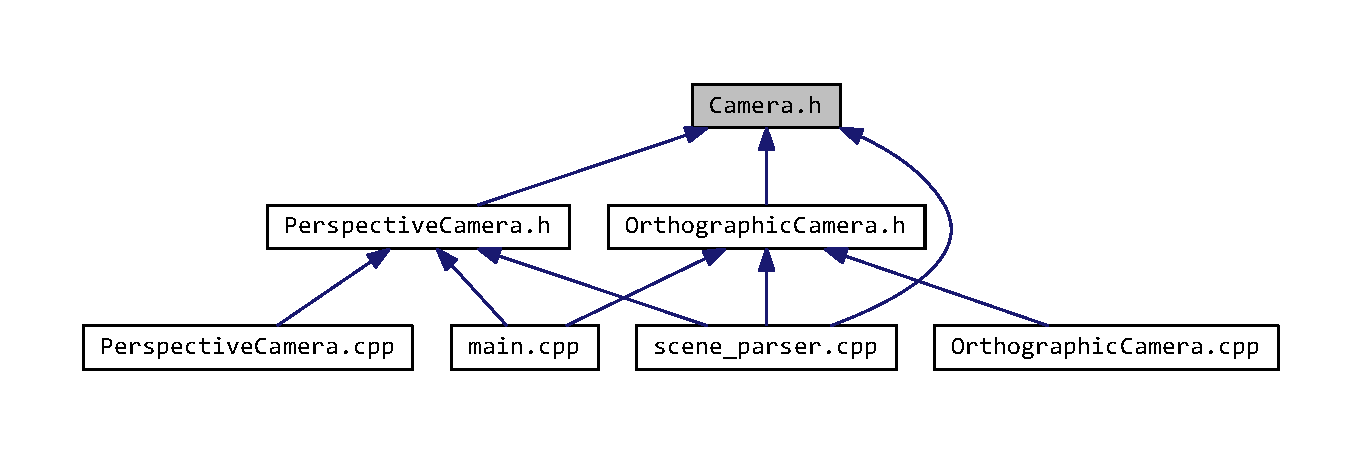
\includegraphics[width=350pt]{Camera_8h__dep__incl}
\end{center}
\end{figure}
\subsection*{Classes}
\begin{DoxyCompactItemize}
\item 
class \hyperlink{classCamera}{Camera}
\end{DoxyCompactItemize}
\subsection*{Enumerations}
\begin{DoxyCompactItemize}
\item 
enum \hyperlink{Camera_8h_af7eb92b45c5f7f64f02821f87c385ebb}{Camera\+Type} \{ \hyperlink{Camera_8h_af7eb92b45c5f7f64f02821f87c385ebba095a1b43effec73955e31e790438de49}{Camera\+Type\+::\+Base}, 
\hyperlink{Camera_8h_af7eb92b45c5f7f64f02821f87c385ebba03424250432f2aa71de95579d2c0eaeb}{Camera\+Type\+::\+Orthographic}, 
\hyperlink{Camera_8h_af7eb92b45c5f7f64f02821f87c385ebbaa80420eef88d11f77532f1b9cb467fa3}{Camera\+Type\+::\+Perspective}
 \}
\end{DoxyCompactItemize}


\subsection{Enumeration Type Documentation}
\hypertarget{Camera_8h_af7eb92b45c5f7f64f02821f87c385ebb}{\index{Camera.\+h@{Camera.\+h}!Camera\+Type@{Camera\+Type}}
\index{Camera\+Type@{Camera\+Type}!Camera.\+h@{Camera.\+h}}
\subsubsection[{Camera\+Type}]{\setlength{\rightskip}{0pt plus 5cm}enum {\bf Camera\+Type}\hspace{0.3cm}{\ttfamily [strong]}}}\label{Camera_8h_af7eb92b45c5f7f64f02821f87c385ebb}
\begin{Desc}
\item[Enumerator]\par
\begin{description}
\index{Base@{Base}!Camera.\+h@{Camera.\+h}}\index{Camera.\+h@{Camera.\+h}!Base@{Base}}\item[{\em 
\hypertarget{Camera_8h_af7eb92b45c5f7f64f02821f87c385ebba095a1b43effec73955e31e790438de49}{Base}\label{Camera_8h_af7eb92b45c5f7f64f02821f87c385ebba095a1b43effec73955e31e790438de49}
}]\index{Orthographic@{Orthographic}!Camera.\+h@{Camera.\+h}}\index{Camera.\+h@{Camera.\+h}!Orthographic@{Orthographic}}\item[{\em 
\hypertarget{Camera_8h_af7eb92b45c5f7f64f02821f87c385ebba03424250432f2aa71de95579d2c0eaeb}{Orthographic}\label{Camera_8h_af7eb92b45c5f7f64f02821f87c385ebba03424250432f2aa71de95579d2c0eaeb}
}]\index{Perspective@{Perspective}!Camera.\+h@{Camera.\+h}}\index{Camera.\+h@{Camera.\+h}!Perspective@{Perspective}}\item[{\em 
\hypertarget{Camera_8h_af7eb92b45c5f7f64f02821f87c385ebbaa80420eef88d11f77532f1b9cb467fa3}{Perspective}\label{Camera_8h_af7eb92b45c5f7f64f02821f87c385ebbaa80420eef88d11f77532f1b9cb467fa3}
}]\end{description}
\end{Desc}

\hypertarget{Group_8cpp}{\section{Group.\+cpp File Reference}
\label{Group_8cpp}\index{Group.\+cpp@{Group.\+cpp}}
}
{\ttfamily \#include \char`\"{}Group.\+h\char`\"{}}\\*
{\ttfamily \#include \char`\"{}hit.\+h\char`\"{}}\\*
Include dependency graph for Group.\+cpp\+:
\nopagebreak
\begin{figure}[H]
\begin{center}
\leavevmode
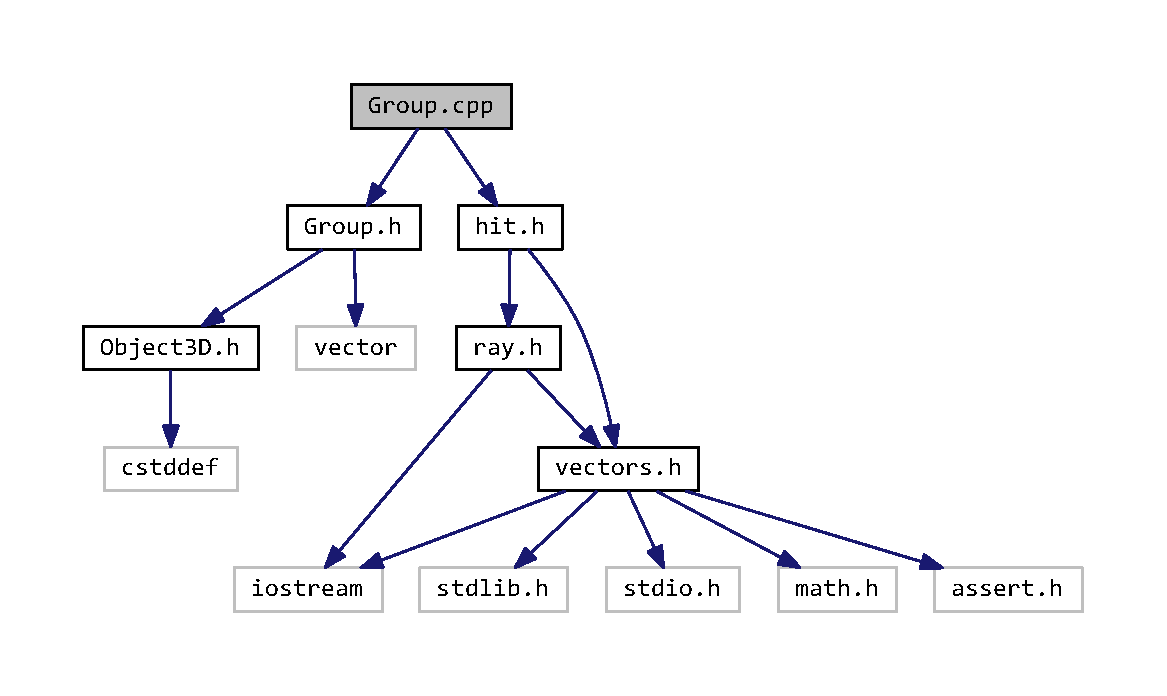
\includegraphics[width=350pt]{Group_8cpp__incl}
\end{center}
\end{figure}

\hypertarget{Group_8h}{\section{Group.\+h File Reference}
\label{Group_8h}\index{Group.\+h@{Group.\+h}}
}
{\ttfamily \#include \char`\"{}Object3\+D.\+h\char`\"{}}\\*
{\ttfamily \#include $<$vector$>$}\\*
Include dependency graph for Group.\+h\+:
\nopagebreak
\begin{figure}[H]
\begin{center}
\leavevmode
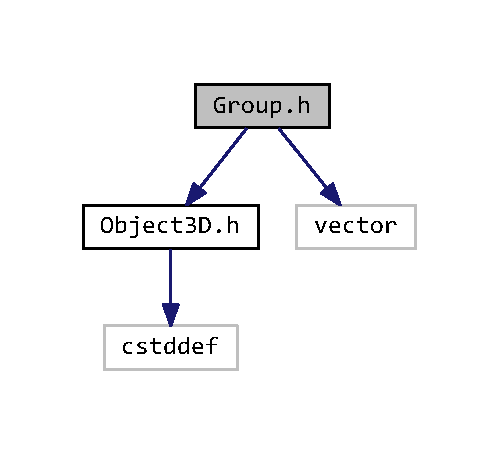
\includegraphics[width=240pt]{Group_8h__incl}
\end{center}
\end{figure}
This graph shows which files directly or indirectly include this file\+:
\nopagebreak
\begin{figure}[H]
\begin{center}
\leavevmode
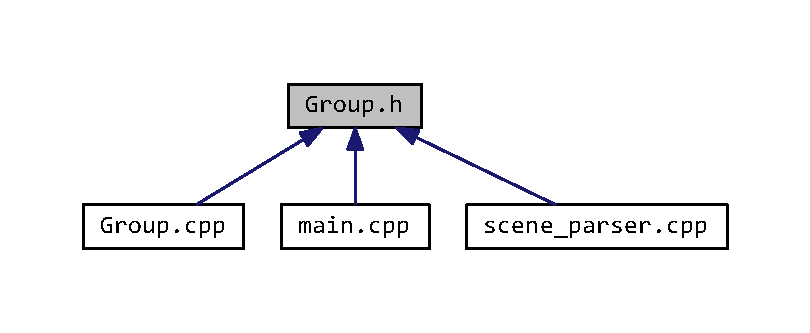
\includegraphics[width=350pt]{Group_8h__dep__incl}
\end{center}
\end{figure}
\subsection*{Classes}
\begin{DoxyCompactItemize}
\item 
class \hyperlink{classGroup}{Group}
\end{DoxyCompactItemize}

\hypertarget{hit_8h}{\section{hit.\+h File Reference}
\label{hit_8h}\index{hit.\+h@{hit.\+h}}
}
{\ttfamily \#include \char`\"{}vectors.\+h\char`\"{}}\\*
{\ttfamily \#include \char`\"{}ray.\+h\char`\"{}}\\*
Include dependency graph for hit.\+h\+:
\nopagebreak
\begin{figure}[H]
\begin{center}
\leavevmode
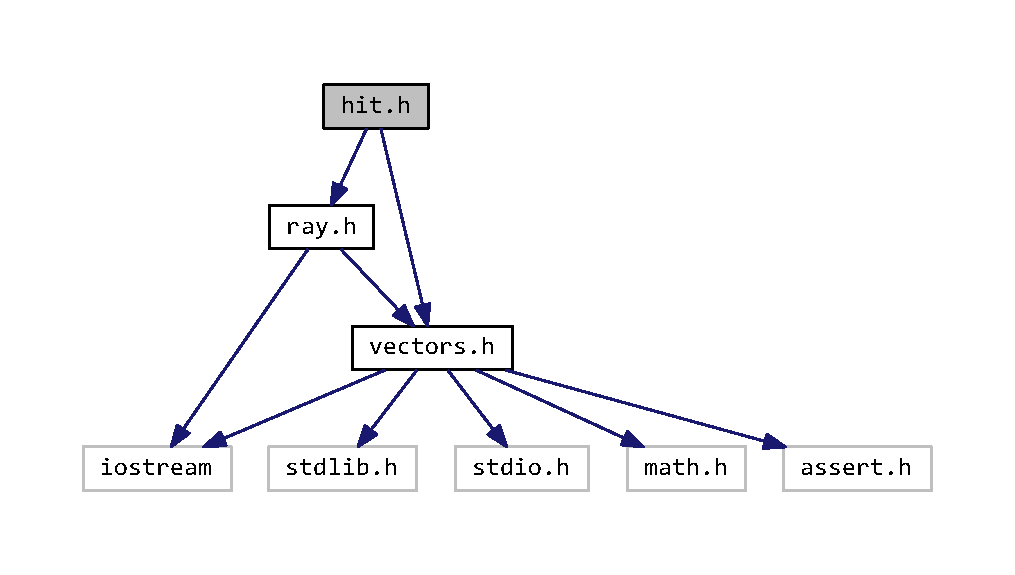
\includegraphics[width=350pt]{hit_8h__incl}
\end{center}
\end{figure}
This graph shows which files directly or indirectly include this file\+:
\nopagebreak
\begin{figure}[H]
\begin{center}
\leavevmode
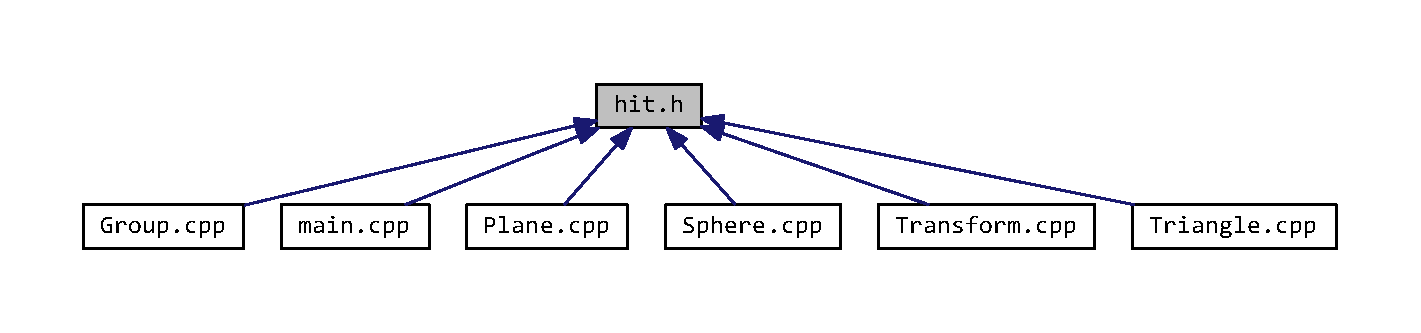
\includegraphics[width=350pt]{hit_8h__dep__incl}
\end{center}
\end{figure}
\subsection*{Classes}
\begin{DoxyCompactItemize}
\item 
class \hyperlink{classHit}{Hit}
\end{DoxyCompactItemize}
\subsection*{Functions}
\begin{DoxyCompactItemize}
\item 
ostream \& \hyperlink{hit_8h_af7c097ea95ecef5a1d1f8aec8c00476f}{operator$<$$<$} (ostream \&os, const \hyperlink{classHit}{Hit} \&h)
\end{DoxyCompactItemize}


\subsection{Function Documentation}
\hypertarget{hit_8h_af7c097ea95ecef5a1d1f8aec8c00476f}{\index{hit.\+h@{hit.\+h}!operator$<$$<$@{operator$<$$<$}}
\index{operator$<$$<$@{operator$<$$<$}!hit.\+h@{hit.\+h}}
\subsubsection[{operator$<$$<$}]{\setlength{\rightskip}{0pt plus 5cm}ostream\& operator$<$$<$ (
\begin{DoxyParamCaption}
\item[{ostream \&}]{os, }
\item[{const {\bf Hit} \&}]{h}
\end{DoxyParamCaption}
)\hspace{0.3cm}{\ttfamily [inline]}}}\label{hit_8h_af7c097ea95ecef5a1d1f8aec8c00476f}

\hypertarget{image_8cpp}{\section{image.\+cpp File Reference}
\label{image_8cpp}\index{image.\+cpp@{image.\+cpp}}
}
{\ttfamily \#include $<$stdlib.\+h$>$}\\*
{\ttfamily \#include $<$stdio.\+h$>$}\\*
{\ttfamily \#include $<$string.\+h$>$}\\*
{\ttfamily \#include \char`\"{}image.\+h\char`\"{}}\\*
Include dependency graph for image.\+cpp\+:
\nopagebreak
\begin{figure}[H]
\begin{center}
\leavevmode
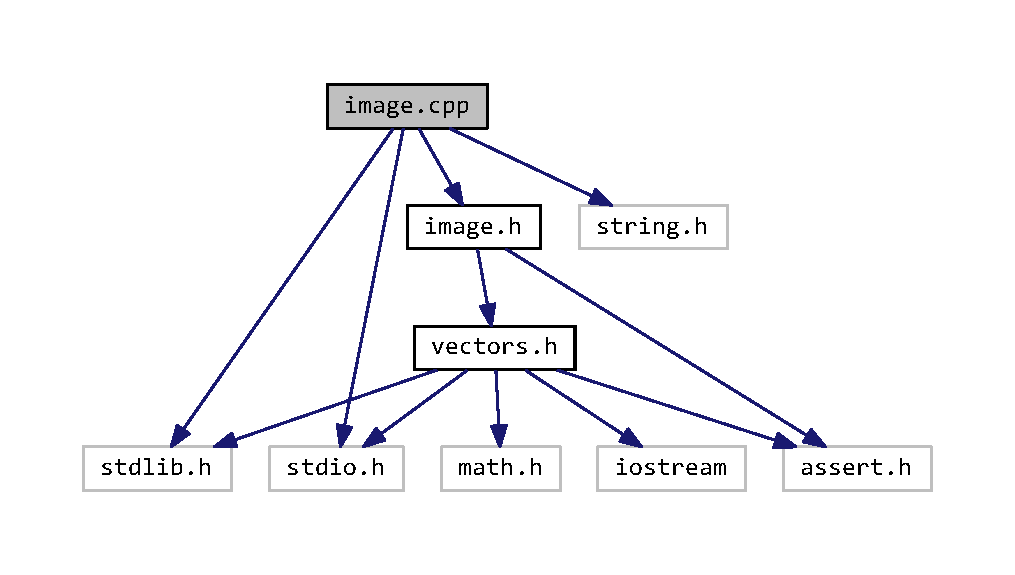
\includegraphics[width=350pt]{image_8cpp__incl}
\end{center}
\end{figure}
\subsection*{Functions}
\begin{DoxyCompactItemize}
\item 
unsigned char \hyperlink{image_8cpp_aac4ea222efb76e9201940fd2fa64bf58}{Read\+Byte} (F\+I\+L\+E $\ast$file)
\item 
void \hyperlink{image_8cpp_a2a66ad4bdcb3bccd8c28d6b5a270c27a}{Write\+Byte} (F\+I\+L\+E $\ast$file, unsigned char b)
\item 
unsigned char \hyperlink{image_8cpp_ac65c2aba23dbe3b80d4d971808494cd8}{Clamp\+Color\+Component} (float c)
\end{DoxyCompactItemize}


\subsection{Function Documentation}
\hypertarget{image_8cpp_ac65c2aba23dbe3b80d4d971808494cd8}{\index{image.\+cpp@{image.\+cpp}!Clamp\+Color\+Component@{Clamp\+Color\+Component}}
\index{Clamp\+Color\+Component@{Clamp\+Color\+Component}!image.\+cpp@{image.\+cpp}}
\subsubsection[{Clamp\+Color\+Component}]{\setlength{\rightskip}{0pt plus 5cm}unsigned char Clamp\+Color\+Component (
\begin{DoxyParamCaption}
\item[{float}]{c}
\end{DoxyParamCaption}
)}}\label{image_8cpp_ac65c2aba23dbe3b80d4d971808494cd8}
\hypertarget{image_8cpp_aac4ea222efb76e9201940fd2fa64bf58}{\index{image.\+cpp@{image.\+cpp}!Read\+Byte@{Read\+Byte}}
\index{Read\+Byte@{Read\+Byte}!image.\+cpp@{image.\+cpp}}
\subsubsection[{Read\+Byte}]{\setlength{\rightskip}{0pt plus 5cm}unsigned char Read\+Byte (
\begin{DoxyParamCaption}
\item[{F\+I\+L\+E $\ast$}]{file}
\end{DoxyParamCaption}
)}}\label{image_8cpp_aac4ea222efb76e9201940fd2fa64bf58}
\hypertarget{image_8cpp_a2a66ad4bdcb3bccd8c28d6b5a270c27a}{\index{image.\+cpp@{image.\+cpp}!Write\+Byte@{Write\+Byte}}
\index{Write\+Byte@{Write\+Byte}!image.\+cpp@{image.\+cpp}}
\subsubsection[{Write\+Byte}]{\setlength{\rightskip}{0pt plus 5cm}void Write\+Byte (
\begin{DoxyParamCaption}
\item[{F\+I\+L\+E $\ast$}]{file, }
\item[{unsigned char}]{b}
\end{DoxyParamCaption}
)}}\label{image_8cpp_a2a66ad4bdcb3bccd8c28d6b5a270c27a}

\hypertarget{image_8h}{\section{image.\+h File Reference}
\label{image_8h}\index{image.\+h@{image.\+h}}
}
{\ttfamily \#include $<$assert.\+h$>$}\\*
{\ttfamily \#include \char`\"{}vectors.\+h\char`\"{}}\\*
Include dependency graph for image.\+h\+:
\nopagebreak
\begin{figure}[H]
\begin{center}
\leavevmode
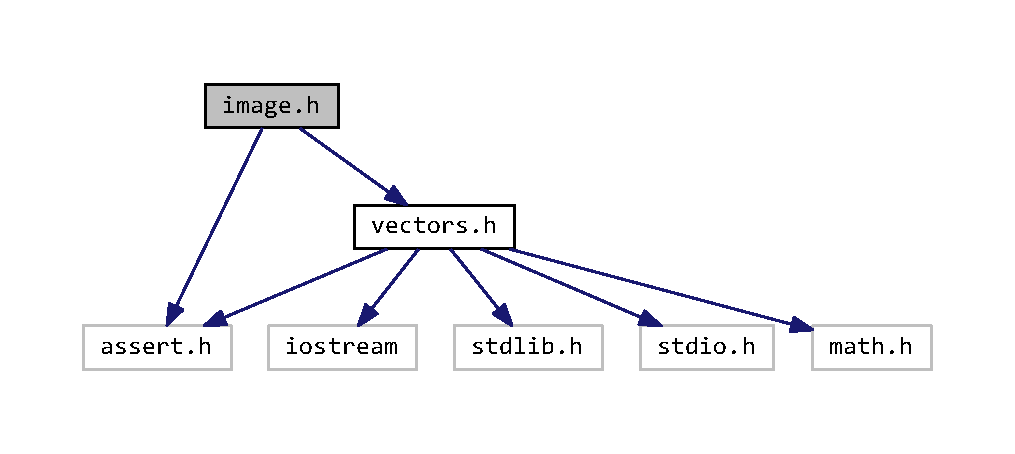
\includegraphics[width=350pt]{image_8h__incl}
\end{center}
\end{figure}
This graph shows which files directly or indirectly include this file\+:
\nopagebreak
\begin{figure}[H]
\begin{center}
\leavevmode
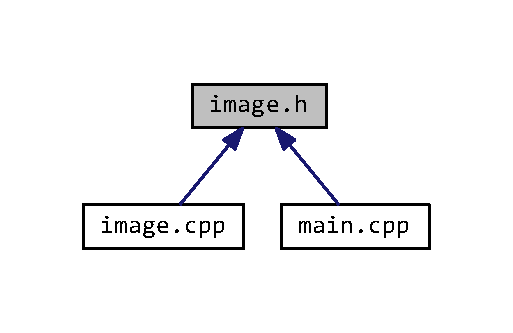
\includegraphics[width=246pt]{image_8h__dep__incl}
\end{center}
\end{figure}
\subsection*{Classes}
\begin{DoxyCompactItemize}
\item 
class \hyperlink{classImage}{Image}
\end{DoxyCompactItemize}

\hypertarget{light_8h}{\section{light.\+h File Reference}
\label{light_8h}\index{light.\+h@{light.\+h}}
}
{\ttfamily \#include \char`\"{}vectors.\+h\char`\"{}}\\*
{\ttfamily \#include \char`\"{}Object3\+D.\+h\char`\"{}}\\*
Include dependency graph for light.\+h\+:
\nopagebreak
\begin{figure}[H]
\begin{center}
\leavevmode
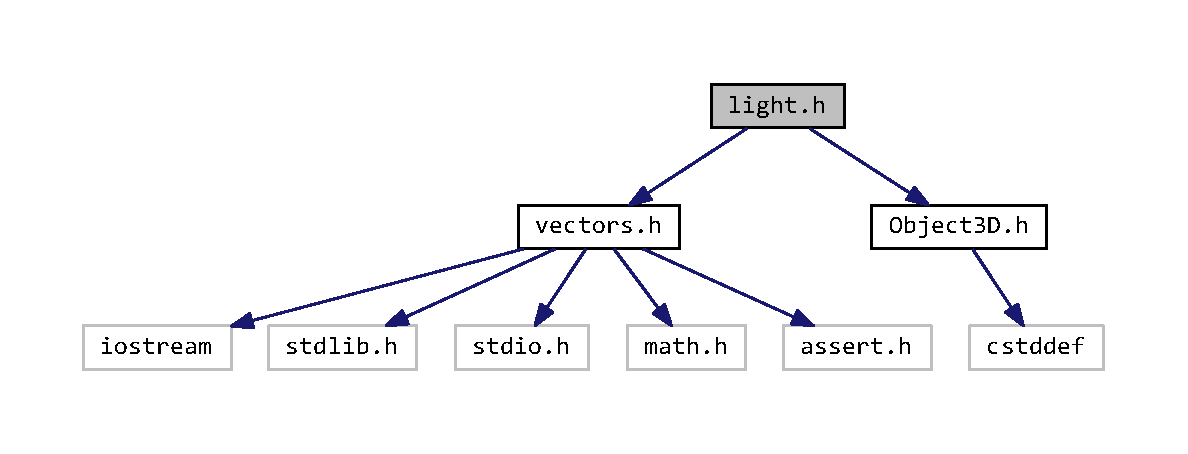
\includegraphics[width=350pt]{light_8h__incl}
\end{center}
\end{figure}
This graph shows which files directly or indirectly include this file\+:
\nopagebreak
\begin{figure}[H]
\begin{center}
\leavevmode
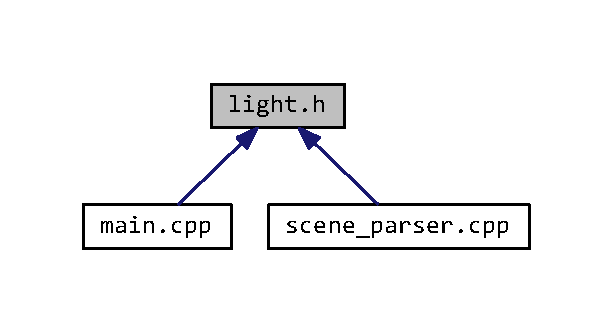
\includegraphics[width=294pt]{light_8h__dep__incl}
\end{center}
\end{figure}
\subsection*{Classes}
\begin{DoxyCompactItemize}
\item 
class \hyperlink{classLight}{Light}
\item 
class \hyperlink{classDirectionalLight}{Directional\+Light}
\end{DoxyCompactItemize}

\hypertarget{main_8cpp}{\section{main.\+cpp File Reference}
\label{main_8cpp}\index{main.\+cpp@{main.\+cpp}}
}
{\ttfamily \#include $<$stdio.\+h$>$}\\*
{\ttfamily \#include $<$string.\+h$>$}\\*
{\ttfamily \#include \char`\"{}scene\+\_\+parser.\+h\char`\"{}}\\*
{\ttfamily \#include \char`\"{}Orthographic\+Camera.\+h\char`\"{}}\\*
{\ttfamily \#include \char`\"{}Perspective\+Camera.\+h\char`\"{}}\\*
{\ttfamily \#include \char`\"{}Group.\+h\char`\"{}}\\*
{\ttfamily \#include \char`\"{}image.\+h\char`\"{}}\\*
{\ttfamily \#include \char`\"{}hit.\+h\char`\"{}}\\*
{\ttfamily \#include \char`\"{}material.\+h\char`\"{}}\\*
{\ttfamily \#include \char`\"{}light.\+h\char`\"{}}\\*
Include dependency graph for main.\+cpp\+:
\nopagebreak
\begin{figure}[H]
\begin{center}
\leavevmode
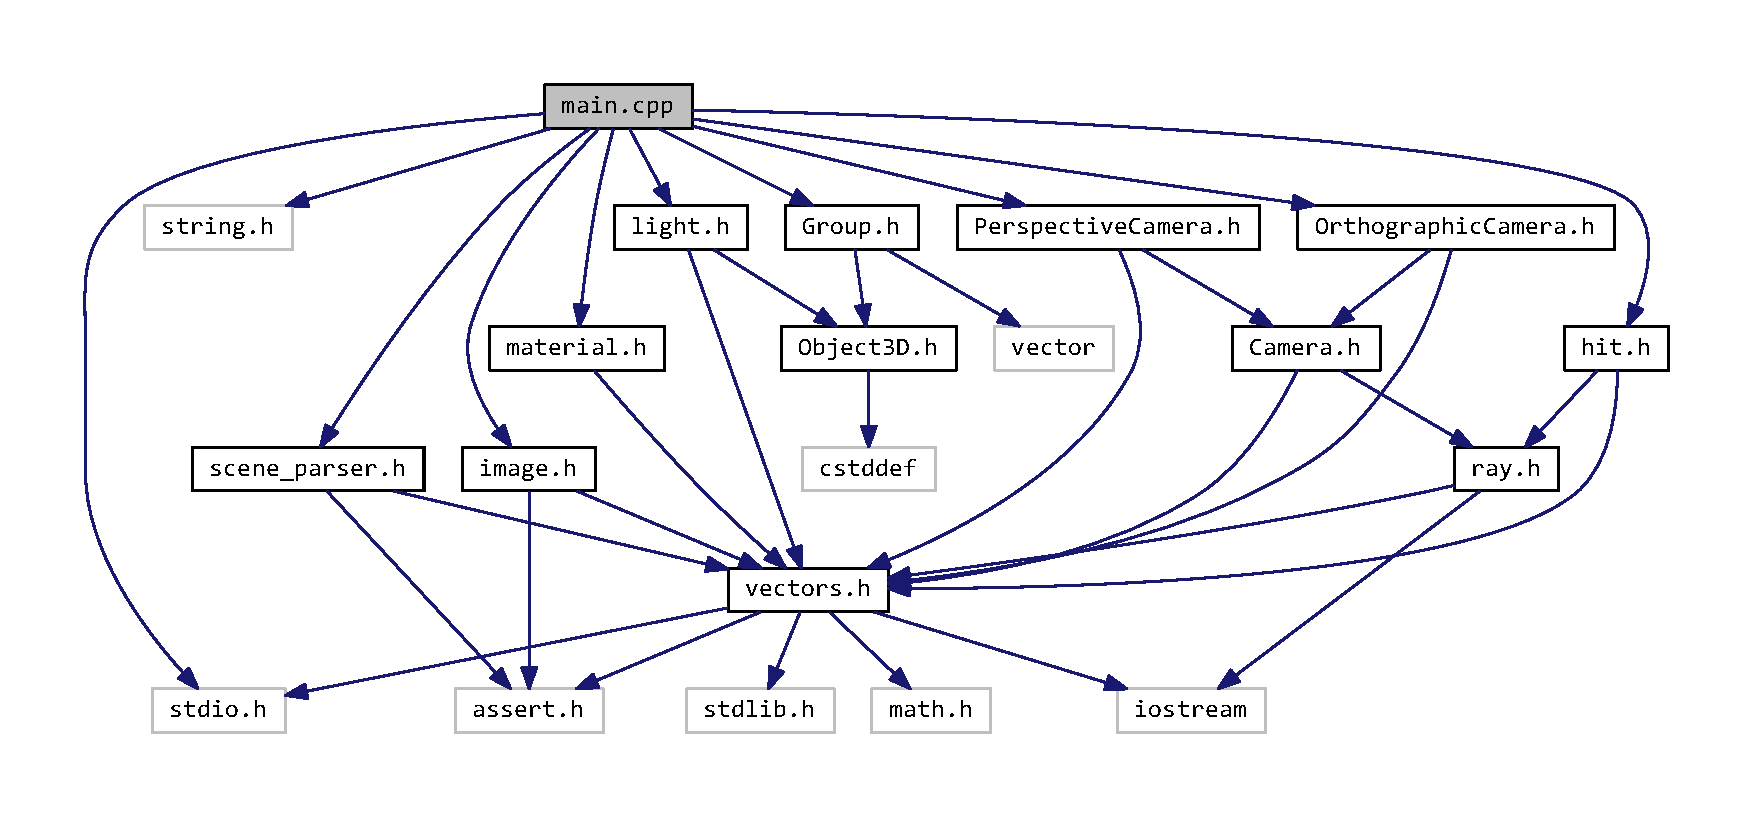
\includegraphics[width=350pt]{main_8cpp__incl}
\end{center}
\end{figure}
\subsection*{Functions}
\begin{DoxyCompactItemize}
\item 
int \hyperlink{main_8cpp_a3c04138a5bfe5d72780bb7e82a18e627}{main} (int argc, char $\ast$$\ast$argv)
\end{DoxyCompactItemize}


\subsection{Function Documentation}
\hypertarget{main_8cpp_a3c04138a5bfe5d72780bb7e82a18e627}{\index{main.\+cpp@{main.\+cpp}!main@{main}}
\index{main@{main}!main.\+cpp@{main.\+cpp}}
\subsubsection[{main}]{\setlength{\rightskip}{0pt plus 5cm}int main (
\begin{DoxyParamCaption}
\item[{int}]{argc, }
\item[{char $\ast$$\ast$}]{argv}
\end{DoxyParamCaption}
)}}\label{main_8cpp_a3c04138a5bfe5d72780bb7e82a18e627}

\hypertarget{material_8h}{\section{material.\+h File Reference}
\label{material_8h}\index{material.\+h@{material.\+h}}
}
{\ttfamily \#include \char`\"{}vectors.\+h\char`\"{}}\\*
Include dependency graph for material.\+h\+:
\nopagebreak
\begin{figure}[H]
\begin{center}
\leavevmode
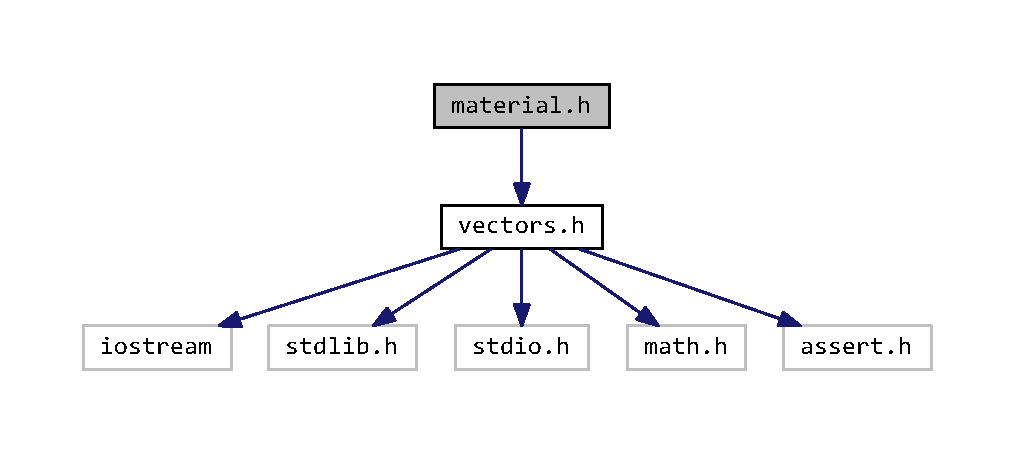
\includegraphics[width=350pt]{material_8h__incl}
\end{center}
\end{figure}
This graph shows which files directly or indirectly include this file\+:
\nopagebreak
\begin{figure}[H]
\begin{center}
\leavevmode
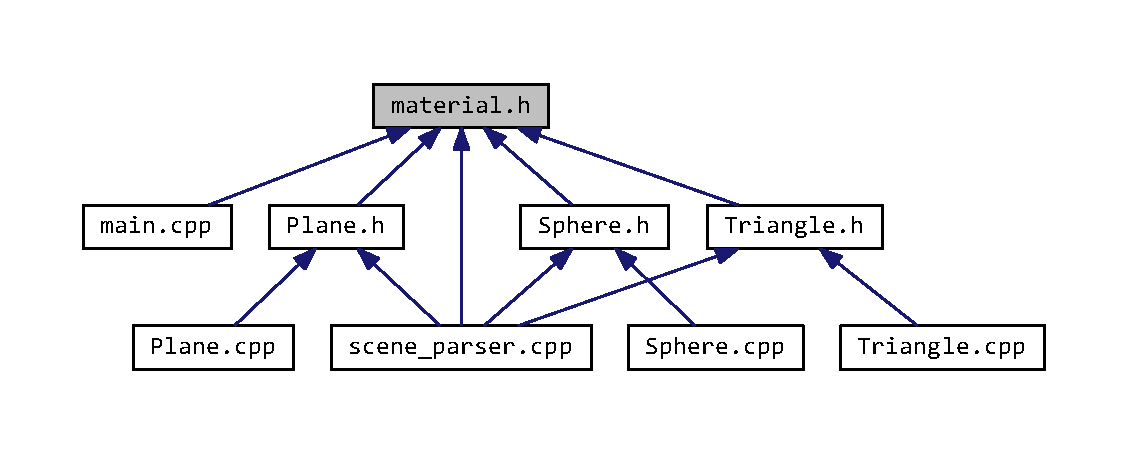
\includegraphics[width=350pt]{material_8h__dep__incl}
\end{center}
\end{figure}
\subsection*{Classes}
\begin{DoxyCompactItemize}
\item 
class \hyperlink{classMaterial}{Material}
\end{DoxyCompactItemize}

\hypertarget{matrix_8cpp}{\section{matrix.\+cpp File Reference}
\label{matrix_8cpp}\index{matrix.\+cpp@{matrix.\+cpp}}
}
{\ttfamily \#include $<$stdlib.\+h$>$}\\*
{\ttfamily \#include $<$stdio.\+h$>$}\\*
{\ttfamily \#include $<$math.\+h$>$}\\*
{\ttfamily \#include $<$string.\+h$>$}\\*
{\ttfamily \#include \char`\"{}matrix.\+h\char`\"{}}\\*
{\ttfamily \#include \char`\"{}vectors.\+h\char`\"{}}\\*
Include dependency graph for matrix.\+cpp\+:
\nopagebreak
\begin{figure}[H]
\begin{center}
\leavevmode
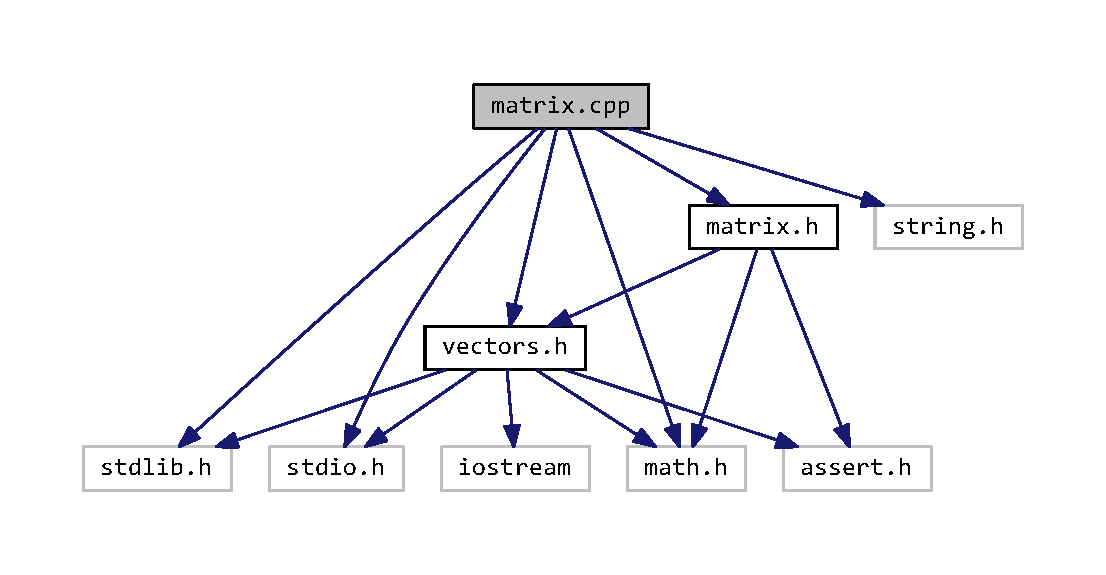
\includegraphics[width=350pt]{matrix_8cpp__incl}
\end{center}
\end{figure}
\subsection*{Functions}
\begin{DoxyCompactItemize}
\item 
float \hyperlink{matrix_8cpp_a2026efe1acd00677b39e6ae710eaf945}{det4x4} (float a1, float a2, float a3, float a4, float b1, float b2, float b3, float b4, float c1, float c2, float c3, float c4, float d1, float d2, float d3, float d4)
\item 
float \hyperlink{matrix_8cpp_a51f32abaa7e4afcf2a10357d61413b68}{det3x3} (float a1, float a2, float a3, float b1, float b2, float b3, float c1, float c2, float c3)
\item 
float \hyperlink{matrix_8cpp_ac1d2ee8881805ada95b910fddba16700}{det2x2} (float a, float b, float c, float d)
\item 
\hyperlink{classMatrix}{Matrix} \hyperlink{matrix_8cpp_aa5a9f2db2b3c1862c9c0d19241239ce7}{operator+} (const \hyperlink{classMatrix}{Matrix} \&m1, const \hyperlink{classMatrix}{Matrix} \&m2)
\item 
\hyperlink{classMatrix}{Matrix} \hyperlink{matrix_8cpp_a52ad5ef4b9998529c85e8523c20d6b86}{operator-\/} (const \hyperlink{classMatrix}{Matrix} \&m1, const \hyperlink{classMatrix}{Matrix} \&m2)
\item 
\hyperlink{classMatrix}{Matrix} \hyperlink{matrix_8cpp_a24da5fd1a21f5010ee32de71af9be3b9}{operator$\ast$} (const \hyperlink{classMatrix}{Matrix} \&m1, const \hyperlink{classMatrix}{Matrix} \&m2)
\item 
\hyperlink{classMatrix}{Matrix} \hyperlink{matrix_8cpp_a4e6d4d99ea83423ef011e7e75094e79e}{operator$\ast$} (const \hyperlink{classMatrix}{Matrix} \&m, float f)
\end{DoxyCompactItemize}


\subsection{Function Documentation}
\hypertarget{matrix_8cpp_ac1d2ee8881805ada95b910fddba16700}{\index{matrix.\+cpp@{matrix.\+cpp}!det2x2@{det2x2}}
\index{det2x2@{det2x2}!matrix.\+cpp@{matrix.\+cpp}}
\subsubsection[{det2x2}]{\setlength{\rightskip}{0pt plus 5cm}float det2x2 (
\begin{DoxyParamCaption}
\item[{float}]{a, }
\item[{float}]{b, }
\item[{float}]{c, }
\item[{float}]{d}
\end{DoxyParamCaption}
)}}\label{matrix_8cpp_ac1d2ee8881805ada95b910fddba16700}
\hypertarget{matrix_8cpp_a51f32abaa7e4afcf2a10357d61413b68}{\index{matrix.\+cpp@{matrix.\+cpp}!det3x3@{det3x3}}
\index{det3x3@{det3x3}!matrix.\+cpp@{matrix.\+cpp}}
\subsubsection[{det3x3}]{\setlength{\rightskip}{0pt plus 5cm}float det3x3 (
\begin{DoxyParamCaption}
\item[{float}]{a1, }
\item[{float}]{a2, }
\item[{float}]{a3, }
\item[{float}]{b1, }
\item[{float}]{b2, }
\item[{float}]{b3, }
\item[{float}]{c1, }
\item[{float}]{c2, }
\item[{float}]{c3}
\end{DoxyParamCaption}
)}}\label{matrix_8cpp_a51f32abaa7e4afcf2a10357d61413b68}
\hypertarget{matrix_8cpp_a2026efe1acd00677b39e6ae710eaf945}{\index{matrix.\+cpp@{matrix.\+cpp}!det4x4@{det4x4}}
\index{det4x4@{det4x4}!matrix.\+cpp@{matrix.\+cpp}}
\subsubsection[{det4x4}]{\setlength{\rightskip}{0pt plus 5cm}float det4x4 (
\begin{DoxyParamCaption}
\item[{float}]{a1, }
\item[{float}]{a2, }
\item[{float}]{a3, }
\item[{float}]{a4, }
\item[{float}]{b1, }
\item[{float}]{b2, }
\item[{float}]{b3, }
\item[{float}]{b4, }
\item[{float}]{c1, }
\item[{float}]{c2, }
\item[{float}]{c3, }
\item[{float}]{c4, }
\item[{float}]{d1, }
\item[{float}]{d2, }
\item[{float}]{d3, }
\item[{float}]{d4}
\end{DoxyParamCaption}
)}}\label{matrix_8cpp_a2026efe1acd00677b39e6ae710eaf945}
\hypertarget{matrix_8cpp_a24da5fd1a21f5010ee32de71af9be3b9}{\index{matrix.\+cpp@{matrix.\+cpp}!operator$\ast$@{operator$\ast$}}
\index{operator$\ast$@{operator$\ast$}!matrix.\+cpp@{matrix.\+cpp}}
\subsubsection[{operator$\ast$}]{\setlength{\rightskip}{0pt plus 5cm}{\bf Matrix} operator$\ast$ (
\begin{DoxyParamCaption}
\item[{const {\bf Matrix} \&}]{m1, }
\item[{const {\bf Matrix} \&}]{m2}
\end{DoxyParamCaption}
)}}\label{matrix_8cpp_a24da5fd1a21f5010ee32de71af9be3b9}
\hypertarget{matrix_8cpp_a4e6d4d99ea83423ef011e7e75094e79e}{\index{matrix.\+cpp@{matrix.\+cpp}!operator$\ast$@{operator$\ast$}}
\index{operator$\ast$@{operator$\ast$}!matrix.\+cpp@{matrix.\+cpp}}
\subsubsection[{operator$\ast$}]{\setlength{\rightskip}{0pt plus 5cm}{\bf Matrix} operator$\ast$ (
\begin{DoxyParamCaption}
\item[{const {\bf Matrix} \&}]{m, }
\item[{float}]{f}
\end{DoxyParamCaption}
)}}\label{matrix_8cpp_a4e6d4d99ea83423ef011e7e75094e79e}
\hypertarget{matrix_8cpp_aa5a9f2db2b3c1862c9c0d19241239ce7}{\index{matrix.\+cpp@{matrix.\+cpp}!operator+@{operator+}}
\index{operator+@{operator+}!matrix.\+cpp@{matrix.\+cpp}}
\subsubsection[{operator+}]{\setlength{\rightskip}{0pt plus 5cm}{\bf Matrix} operator+ (
\begin{DoxyParamCaption}
\item[{const {\bf Matrix} \&}]{m1, }
\item[{const {\bf Matrix} \&}]{m2}
\end{DoxyParamCaption}
)}}\label{matrix_8cpp_aa5a9f2db2b3c1862c9c0d19241239ce7}
\hypertarget{matrix_8cpp_a52ad5ef4b9998529c85e8523c20d6b86}{\index{matrix.\+cpp@{matrix.\+cpp}!operator-\/@{operator-\/}}
\index{operator-\/@{operator-\/}!matrix.\+cpp@{matrix.\+cpp}}
\subsubsection[{operator-\/}]{\setlength{\rightskip}{0pt plus 5cm}{\bf Matrix} operator-\/ (
\begin{DoxyParamCaption}
\item[{const {\bf Matrix} \&}]{m1, }
\item[{const {\bf Matrix} \&}]{m2}
\end{DoxyParamCaption}
)}}\label{matrix_8cpp_a52ad5ef4b9998529c85e8523c20d6b86}

\hypertarget{matrix_8h}{\section{matrix.\+h File Reference}
\label{matrix_8h}\index{matrix.\+h@{matrix.\+h}}
}
{\ttfamily \#include $<$math.\+h$>$}\\*
{\ttfamily \#include $<$assert.\+h$>$}\\*
{\ttfamily \#include \char`\"{}vectors.\+h\char`\"{}}\\*
Include dependency graph for matrix.\+h\+:
\nopagebreak
\begin{figure}[H]
\begin{center}
\leavevmode
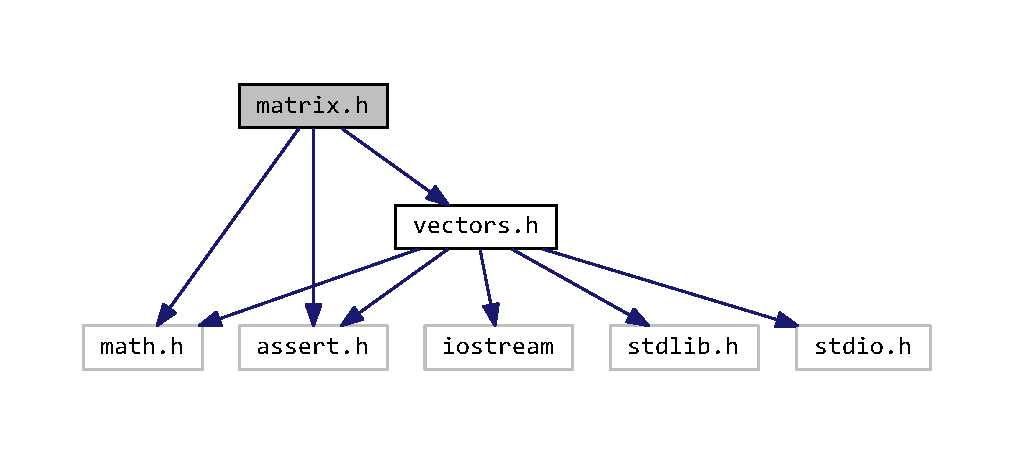
\includegraphics[width=350pt]{matrix_8h__incl}
\end{center}
\end{figure}
This graph shows which files directly or indirectly include this file\+:
\nopagebreak
\begin{figure}[H]
\begin{center}
\leavevmode
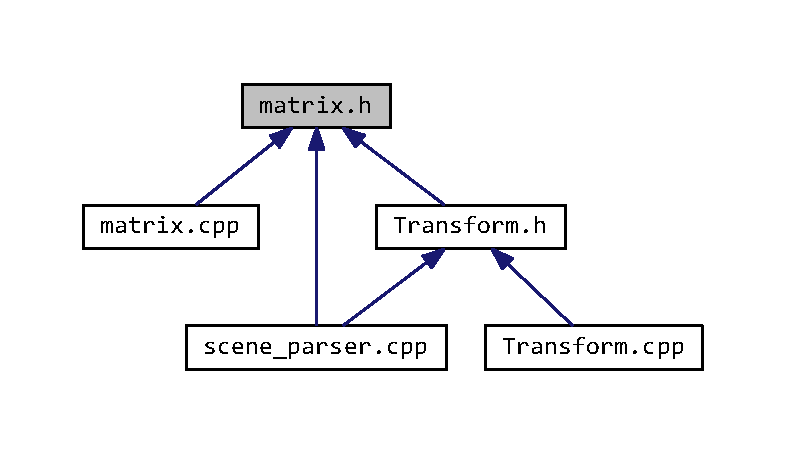
\includegraphics[width=350pt]{matrix_8h__dep__incl}
\end{center}
\end{figure}
\subsection*{Classes}
\begin{DoxyCompactItemize}
\item 
class \hyperlink{classMatrix}{Matrix}
\end{DoxyCompactItemize}

\hypertarget{Object3D_8h}{\section{Object3\+D.\+h File Reference}
\label{Object3D_8h}\index{Object3\+D.\+h@{Object3\+D.\+h}}
}
{\ttfamily \#include $<$cstddef$>$}\\*
Include dependency graph for Object3\+D.\+h\+:
\nopagebreak
\begin{figure}[H]
\begin{center}
\leavevmode
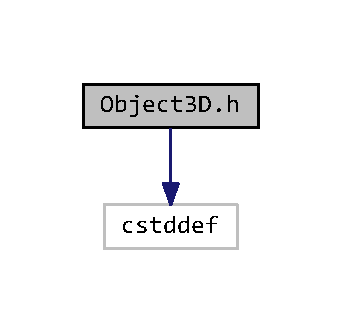
\includegraphics[width=164pt]{Object3D_8h__incl}
\end{center}
\end{figure}
This graph shows which files directly or indirectly include this file\+:
\nopagebreak
\begin{figure}[H]
\begin{center}
\leavevmode
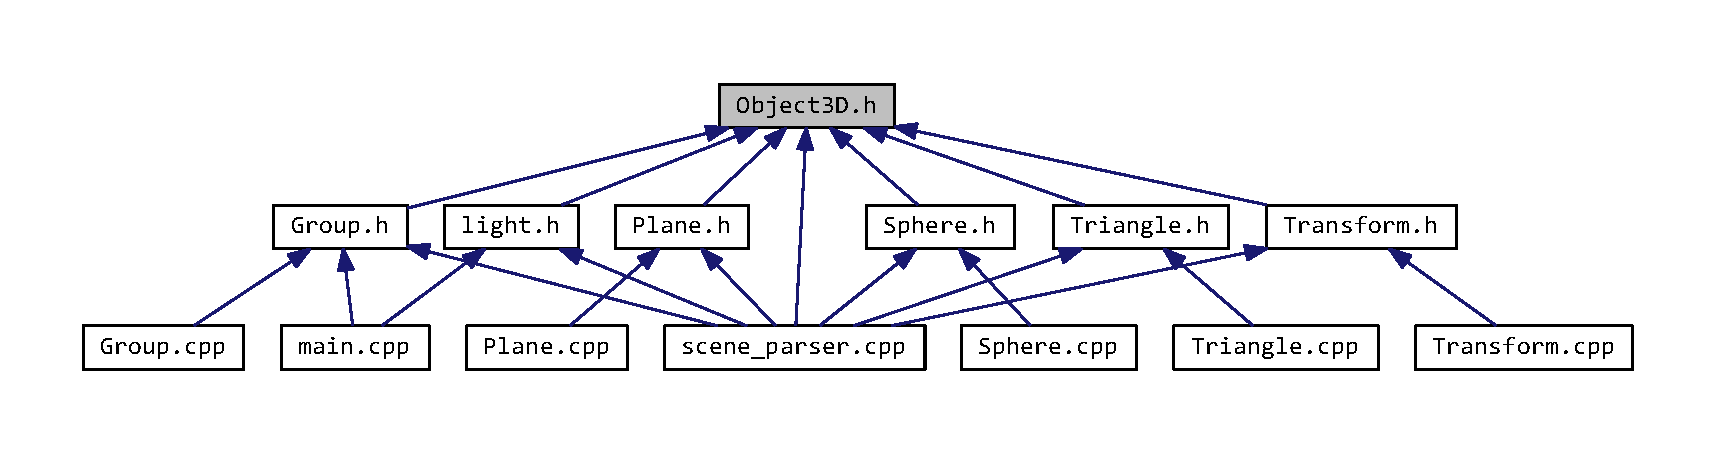
\includegraphics[width=350pt]{Object3D_8h__dep__incl}
\end{center}
\end{figure}
\subsection*{Classes}
\begin{DoxyCompactItemize}
\item 
class \hyperlink{classObject3D}{Object3\+D}
\end{DoxyCompactItemize}

\hypertarget{OrthographicCamera_8cpp}{\section{Orthographic\+Camera.\+cpp File Reference}
\label{OrthographicCamera_8cpp}\index{Orthographic\+Camera.\+cpp@{Orthographic\+Camera.\+cpp}}
}
{\ttfamily \#include \char`\"{}Orthographic\+Camera.\+h\char`\"{}}\\*
Include dependency graph for Orthographic\+Camera.\+cpp\+:
\nopagebreak
\begin{figure}[H]
\begin{center}
\leavevmode
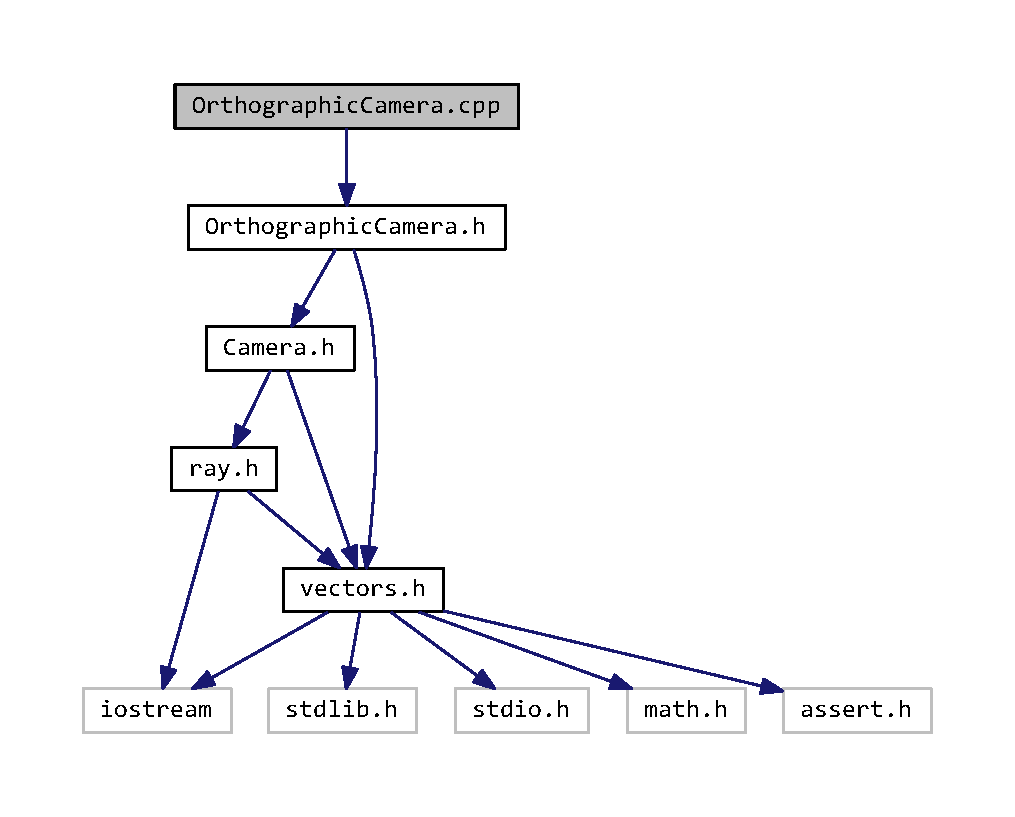
\includegraphics[width=350pt]{OrthographicCamera_8cpp__incl}
\end{center}
\end{figure}
\subsection*{Macros}
\begin{DoxyCompactItemize}
\item 
\#define \hyperlink{OrthographicCamera_8cpp_a0e37b765046be143ca51ec097adf606a}{T\+\_\+\+M\+I\+N}~-\/100000.\+0
\end{DoxyCompactItemize}


\subsection{Macro Definition Documentation}
\hypertarget{OrthographicCamera_8cpp_a0e37b765046be143ca51ec097adf606a}{\index{Orthographic\+Camera.\+cpp@{Orthographic\+Camera.\+cpp}!T\+\_\+\+M\+I\+N@{T\+\_\+\+M\+I\+N}}
\index{T\+\_\+\+M\+I\+N@{T\+\_\+\+M\+I\+N}!Orthographic\+Camera.\+cpp@{Orthographic\+Camera.\+cpp}}
\subsubsection[{T\+\_\+\+M\+I\+N}]{\setlength{\rightskip}{0pt plus 5cm}\#define T\+\_\+\+M\+I\+N~-\/100000.\+0}}\label{OrthographicCamera_8cpp_a0e37b765046be143ca51ec097adf606a}

\hypertarget{OrthographicCamera_8h}{\section{Orthographic\+Camera.\+h File Reference}
\label{OrthographicCamera_8h}\index{Orthographic\+Camera.\+h@{Orthographic\+Camera.\+h}}
}
{\ttfamily \#include \char`\"{}Camera.\+h\char`\"{}}\\*
{\ttfamily \#include \char`\"{}vectors.\+h\char`\"{}}\\*
Include dependency graph for Orthographic\+Camera.\+h\+:
\nopagebreak
\begin{figure}[H]
\begin{center}
\leavevmode
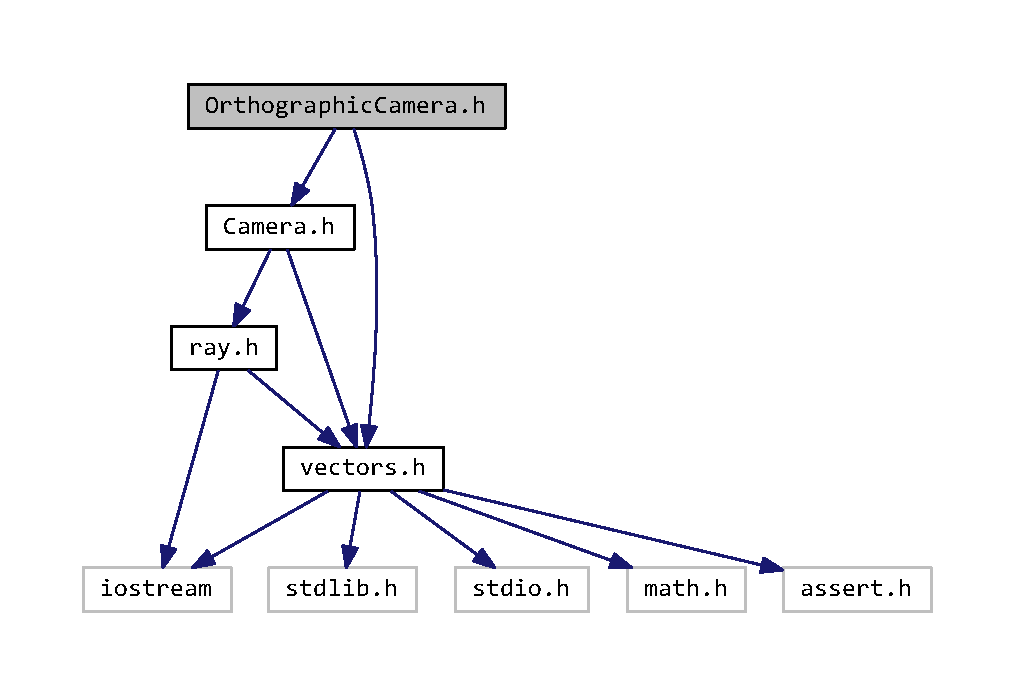
\includegraphics[width=350pt]{OrthographicCamera_8h__incl}
\end{center}
\end{figure}
This graph shows which files directly or indirectly include this file\+:
\nopagebreak
\begin{figure}[H]
\begin{center}
\leavevmode
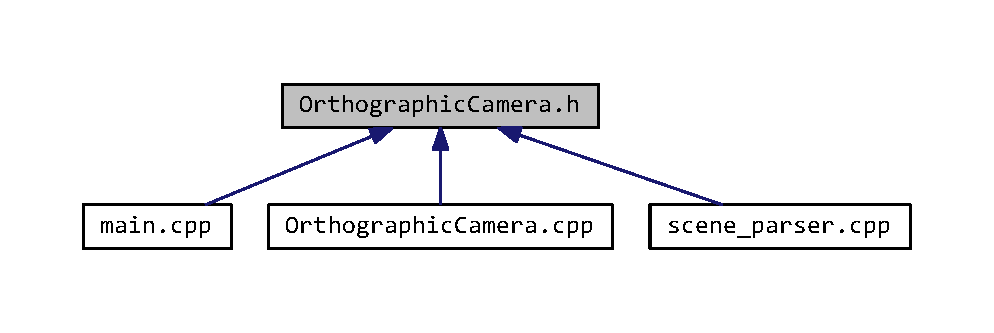
\includegraphics[width=350pt]{OrthographicCamera_8h__dep__incl}
\end{center}
\end{figure}
\subsection*{Classes}
\begin{DoxyCompactItemize}
\item 
class \hyperlink{classOrthographicCamera}{Orthographic\+Camera}
\end{DoxyCompactItemize}

\hypertarget{PerspectiveCamera_8cpp}{\section{Perspective\+Camera.\+cpp File Reference}
\label{PerspectiveCamera_8cpp}\index{Perspective\+Camera.\+cpp@{Perspective\+Camera.\+cpp}}
}
{\ttfamily \#include \char`\"{}Perspective\+Camera.\+h\char`\"{}}\\*
{\ttfamily \#include $<$math.\+h$>$}\\*
Include dependency graph for Perspective\+Camera.\+cpp\+:
\nopagebreak
\begin{figure}[H]
\begin{center}
\leavevmode
\includegraphics[width=350pt]{PerspectiveCamera_8cpp__incl}
\end{center}
\end{figure}
\subsection*{Macros}
\begin{DoxyCompactItemize}
\item 
\#define \hyperlink{PerspectiveCamera_8cpp_a598a3330b3c21701223ee0ca14316eca}{P\+I}~3.\+14159265
\end{DoxyCompactItemize}


\subsection{Macro Definition Documentation}
\hypertarget{PerspectiveCamera_8cpp_a598a3330b3c21701223ee0ca14316eca}{\index{Perspective\+Camera.\+cpp@{Perspective\+Camera.\+cpp}!P\+I@{P\+I}}
\index{P\+I@{P\+I}!Perspective\+Camera.\+cpp@{Perspective\+Camera.\+cpp}}
\subsubsection[{P\+I}]{\setlength{\rightskip}{0pt plus 5cm}\#define P\+I~3.\+14159265}}\label{PerspectiveCamera_8cpp_a598a3330b3c21701223ee0ca14316eca}

\hypertarget{PerspectiveCamera_8h}{\section{Perspective\+Camera.\+h File Reference}
\label{PerspectiveCamera_8h}\index{Perspective\+Camera.\+h@{Perspective\+Camera.\+h}}
}
{\ttfamily \#include \char`\"{}Camera.\+h\char`\"{}}\\*
{\ttfamily \#include \char`\"{}vectors.\+h\char`\"{}}\\*
Include dependency graph for Perspective\+Camera.\+h\+:
\nopagebreak
\begin{figure}[H]
\begin{center}
\leavevmode
\includegraphics[width=350pt]{PerspectiveCamera_8h__incl}
\end{center}
\end{figure}
This graph shows which files directly or indirectly include this file\+:
\nopagebreak
\begin{figure}[H]
\begin{center}
\leavevmode
\includegraphics[width=350pt]{PerspectiveCamera_8h__dep__incl}
\end{center}
\end{figure}
\subsection*{Classes}
\begin{DoxyCompactItemize}
\item 
class \hyperlink{classPerspectiveCamera}{Perspective\+Camera}
\end{DoxyCompactItemize}

\hypertarget{Plane_8cpp}{\section{Plane.\+cpp File Reference}
\label{Plane_8cpp}\index{Plane.\+cpp@{Plane.\+cpp}}
}
{\ttfamily \#include \char`\"{}Plane.\+h\char`\"{}}\\*
{\ttfamily \#include \char`\"{}hit.\+h\char`\"{}}\\*
Include dependency graph for Plane.\+cpp\+:
\nopagebreak
\begin{figure}[H]
\begin{center}
\leavevmode
\includegraphics[width=350pt]{Plane_8cpp__incl}
\end{center}
\end{figure}

\hypertarget{Plane_8h}{\section{Plane.\+h File Reference}
\label{Plane_8h}\index{Plane.\+h@{Plane.\+h}}
}
{\ttfamily \#include \char`\"{}Object3\+D.\+h\char`\"{}}\\*
{\ttfamily \#include \char`\"{}vectors.\+h\char`\"{}}\\*
{\ttfamily \#include \char`\"{}material.\+h\char`\"{}}\\*
Include dependency graph for Plane.\+h\+:
\nopagebreak
\begin{figure}[H]
\begin{center}
\leavevmode
\includegraphics[width=350pt]{Plane_8h__incl}
\end{center}
\end{figure}
This graph shows which files directly or indirectly include this file\+:
\nopagebreak
\begin{figure}[H]
\begin{center}
\leavevmode
\includegraphics[width=300pt]{Plane_8h__dep__incl}
\end{center}
\end{figure}
\subsection*{Classes}
\begin{DoxyCompactItemize}
\item 
class \hyperlink{classPlane}{Plane}
\end{DoxyCompactItemize}

\hypertarget{ray_8h}{\section{ray.\+h File Reference}
\label{ray_8h}\index{ray.\+h@{ray.\+h}}
}
{\ttfamily \#include $<$iostream$>$}\\*
{\ttfamily \#include \char`\"{}vectors.\+h\char`\"{}}\\*
Include dependency graph for ray.\+h\+:
\nopagebreak
\begin{figure}[H]
\begin{center}
\leavevmode
\includegraphics[width=350pt]{ray_8h__incl}
\end{center}
\end{figure}
This graph shows which files directly or indirectly include this file\+:
\nopagebreak
\begin{figure}[H]
\begin{center}
\leavevmode
\includegraphics[width=350pt]{ray_8h__dep__incl}
\end{center}
\end{figure}
\subsection*{Classes}
\begin{DoxyCompactItemize}
\item 
class \hyperlink{classRay}{Ray}
\end{DoxyCompactItemize}
\subsection*{Functions}
\begin{DoxyCompactItemize}
\item 
ostream \& \hyperlink{ray_8h_a58ab17142b3c74a8d39c1e42dfa7a3f4}{operator$<$$<$} (ostream \&os, const \hyperlink{classRay}{Ray} \&r)
\end{DoxyCompactItemize}


\subsection{Function Documentation}
\hypertarget{ray_8h_a58ab17142b3c74a8d39c1e42dfa7a3f4}{\index{ray.\+h@{ray.\+h}!operator$<$$<$@{operator$<$$<$}}
\index{operator$<$$<$@{operator$<$$<$}!ray.\+h@{ray.\+h}}
\subsubsection[{operator$<$$<$}]{\setlength{\rightskip}{0pt plus 5cm}ostream\& operator$<$$<$ (
\begin{DoxyParamCaption}
\item[{ostream \&}]{os, }
\item[{const {\bf Ray} \&}]{r}
\end{DoxyParamCaption}
)\hspace{0.3cm}{\ttfamily [inline]}}}\label{ray_8h_a58ab17142b3c74a8d39c1e42dfa7a3f4}

\hypertarget{scene__parser_8cpp}{\section{scene\+\_\+parser.\+cpp File Reference}
\label{scene__parser_8cpp}\index{scene\+\_\+parser.\+cpp@{scene\+\_\+parser.\+cpp}}
}
{\ttfamily \#include $<$stdio.\+h$>$}\\*
{\ttfamily \#include $<$string.\+h$>$}\\*
{\ttfamily \#include \char`\"{}scene\+\_\+parser.\+h\char`\"{}}\\*
{\ttfamily \#include \char`\"{}matrix.\+h\char`\"{}}\\*
{\ttfamily \#include \char`\"{}Camera.\+h\char`\"{}}\\*
{\ttfamily \#include \char`\"{}Orthographic\+Camera.\+h\char`\"{}}\\*
{\ttfamily \#include \char`\"{}Perspective\+Camera.\+h\char`\"{}}\\*
{\ttfamily \#include \char`\"{}light.\+h\char`\"{}}\\*
{\ttfamily \#include \char`\"{}material.\+h\char`\"{}}\\*
{\ttfamily \#include \char`\"{}Object3\+D.\+h\char`\"{}}\\*
{\ttfamily \#include \char`\"{}Group.\+h\char`\"{}}\\*
{\ttfamily \#include \char`\"{}Sphere.\+h\char`\"{}}\\*
{\ttfamily \#include \char`\"{}Plane.\+h\char`\"{}}\\*
{\ttfamily \#include \char`\"{}Triangle.\+h\char`\"{}}\\*
{\ttfamily \#include \char`\"{}Transform.\+h\char`\"{}}\\*
Include dependency graph for scene\+\_\+parser.\+cpp\+:
\nopagebreak
\begin{figure}[H]
\begin{center}
\leavevmode
\includegraphics[width=350pt]{scene__parser_8cpp__incl}
\end{center}
\end{figure}
\subsection*{Macros}
\begin{DoxyCompactItemize}
\item 
\#define \hyperlink{scene__parser_8cpp_a4b45917df9c2dd996220e6da5b4afa80}{Degrees\+To\+Radians}(x)~((M\+\_\+\+P\+I $\ast$ x) / 180.\+0f)
\end{DoxyCompactItemize}


\subsection{Macro Definition Documentation}
\hypertarget{scene__parser_8cpp_a4b45917df9c2dd996220e6da5b4afa80}{\index{scene\+\_\+parser.\+cpp@{scene\+\_\+parser.\+cpp}!Degrees\+To\+Radians@{Degrees\+To\+Radians}}
\index{Degrees\+To\+Radians@{Degrees\+To\+Radians}!scene\+\_\+parser.\+cpp@{scene\+\_\+parser.\+cpp}}
\subsubsection[{Degrees\+To\+Radians}]{\setlength{\rightskip}{0pt plus 5cm}\#define Degrees\+To\+Radians(
\begin{DoxyParamCaption}
\item[{}]{x}
\end{DoxyParamCaption}
)~((M\+\_\+\+P\+I $\ast$ x) / 180.\+0f)}}\label{scene__parser_8cpp_a4b45917df9c2dd996220e6da5b4afa80}

\hypertarget{scene__parser_8h}{\section{scene\+\_\+parser.\+h File Reference}
\label{scene__parser_8h}\index{scene\+\_\+parser.\+h@{scene\+\_\+parser.\+h}}
}
{\ttfamily \#include \char`\"{}vectors.\+h\char`\"{}}\\*
{\ttfamily \#include $<$assert.\+h$>$}\\*
Include dependency graph for scene\+\_\+parser.\+h\+:
\nopagebreak
\begin{figure}[H]
\begin{center}
\leavevmode
\includegraphics[width=350pt]{scene__parser_8h__incl}
\end{center}
\end{figure}
This graph shows which files directly or indirectly include this file\+:
\nopagebreak
\begin{figure}[H]
\begin{center}
\leavevmode
\includegraphics[width=294pt]{scene__parser_8h__dep__incl}
\end{center}
\end{figure}
\subsection*{Classes}
\begin{DoxyCompactItemize}
\item 
class \hyperlink{classSceneParser}{Scene\+Parser}
\end{DoxyCompactItemize}
\subsection*{Macros}
\begin{DoxyCompactItemize}
\item 
\#define \hyperlink{scene__parser_8h_a1ee17f9bf2ebcfebd7548287b0fe0fe4}{M\+A\+X\+\_\+\+P\+A\+R\+S\+E\+R\+\_\+\+T\+O\+K\+E\+N\+\_\+\+L\+E\+N\+G\+T\+H}~100
\end{DoxyCompactItemize}


\subsection{Macro Definition Documentation}
\hypertarget{scene__parser_8h_a1ee17f9bf2ebcfebd7548287b0fe0fe4}{\index{scene\+\_\+parser.\+h@{scene\+\_\+parser.\+h}!M\+A\+X\+\_\+\+P\+A\+R\+S\+E\+R\+\_\+\+T\+O\+K\+E\+N\+\_\+\+L\+E\+N\+G\+T\+H@{M\+A\+X\+\_\+\+P\+A\+R\+S\+E\+R\+\_\+\+T\+O\+K\+E\+N\+\_\+\+L\+E\+N\+G\+T\+H}}
\index{M\+A\+X\+\_\+\+P\+A\+R\+S\+E\+R\+\_\+\+T\+O\+K\+E\+N\+\_\+\+L\+E\+N\+G\+T\+H@{M\+A\+X\+\_\+\+P\+A\+R\+S\+E\+R\+\_\+\+T\+O\+K\+E\+N\+\_\+\+L\+E\+N\+G\+T\+H}!scene\+\_\+parser.\+h@{scene\+\_\+parser.\+h}}
\subsubsection[{M\+A\+X\+\_\+\+P\+A\+R\+S\+E\+R\+\_\+\+T\+O\+K\+E\+N\+\_\+\+L\+E\+N\+G\+T\+H}]{\setlength{\rightskip}{0pt plus 5cm}\#define M\+A\+X\+\_\+\+P\+A\+R\+S\+E\+R\+\_\+\+T\+O\+K\+E\+N\+\_\+\+L\+E\+N\+G\+T\+H~100}}\label{scene__parser_8h_a1ee17f9bf2ebcfebd7548287b0fe0fe4}

\hypertarget{Sphere_8cpp}{\section{Sphere.\+cpp File Reference}
\label{Sphere_8cpp}\index{Sphere.\+cpp@{Sphere.\+cpp}}
}
{\ttfamily \#include \char`\"{}Sphere.\+h\char`\"{}}\\*
{\ttfamily \#include \char`\"{}hit.\+h\char`\"{}}\\*
Include dependency graph for Sphere.\+cpp\+:
\nopagebreak
\begin{figure}[H]
\begin{center}
\leavevmode
\includegraphics[width=350pt]{Sphere_8cpp__incl}
\end{center}
\end{figure}
\subsection*{Macros}
\begin{DoxyCompactItemize}
\item 
\#define \hyperlink{Sphere_8cpp_acd0dda75fa865e1efae98e3e2b204ef4}{T\+\_\+\+M\+A\+X}~100000.\+0f
\end{DoxyCompactItemize}


\subsection{Macro Definition Documentation}
\hypertarget{Sphere_8cpp_acd0dda75fa865e1efae98e3e2b204ef4}{\index{Sphere.\+cpp@{Sphere.\+cpp}!T\+\_\+\+M\+A\+X@{T\+\_\+\+M\+A\+X}}
\index{T\+\_\+\+M\+A\+X@{T\+\_\+\+M\+A\+X}!Sphere.\+cpp@{Sphere.\+cpp}}
\subsubsection[{T\+\_\+\+M\+A\+X}]{\setlength{\rightskip}{0pt plus 5cm}\#define T\+\_\+\+M\+A\+X~100000.\+0f}}\label{Sphere_8cpp_acd0dda75fa865e1efae98e3e2b204ef4}

\hypertarget{Sphere_8h}{\section{Sphere.\+h File Reference}
\label{Sphere_8h}\index{Sphere.\+h@{Sphere.\+h}}
}
{\ttfamily \#include \char`\"{}Object3\+D.\+h\char`\"{}}\\*
{\ttfamily \#include \char`\"{}vectors.\+h\char`\"{}}\\*
{\ttfamily \#include \char`\"{}material.\+h\char`\"{}}\\*
Include dependency graph for Sphere.\+h\+:
\nopagebreak
\begin{figure}[H]
\begin{center}
\leavevmode
\includegraphics[width=350pt]{Sphere_8h__incl}
\end{center}
\end{figure}
This graph shows which files directly or indirectly include this file\+:
\nopagebreak
\begin{figure}[H]
\begin{center}
\leavevmode
\includegraphics[width=307pt]{Sphere_8h__dep__incl}
\end{center}
\end{figure}
\subsection*{Classes}
\begin{DoxyCompactItemize}
\item 
class \hyperlink{classSphere}{Sphere}
\end{DoxyCompactItemize}

\hypertarget{Transform_8cpp}{\section{Transform.\+cpp File Reference}
\label{Transform_8cpp}\index{Transform.\+cpp@{Transform.\+cpp}}
}
{\ttfamily \#include \char`\"{}Transform.\+h\char`\"{}}\\*
{\ttfamily \#include \char`\"{}hit.\+h\char`\"{}}\\*
Include dependency graph for Transform.\+cpp\+:
\nopagebreak
\begin{figure}[H]
\begin{center}
\leavevmode
\includegraphics[width=350pt]{Transform_8cpp__incl}
\end{center}
\end{figure}

\hypertarget{Transform_8h}{\section{Transform.\+h File Reference}
\label{Transform_8h}\index{Transform.\+h@{Transform.\+h}}
}
{\ttfamily \#include \char`\"{}Object3\+D.\+h\char`\"{}}\\*
{\ttfamily \#include \char`\"{}matrix.\+h\char`\"{}}\\*
Include dependency graph for Transform.\+h\+:
\nopagebreak
\begin{figure}[H]
\begin{center}
\leavevmode
\includegraphics[width=350pt]{Transform_8h__incl}
\end{center}
\end{figure}
This graph shows which files directly or indirectly include this file\+:
\nopagebreak
\begin{figure}[H]
\begin{center}
\leavevmode
\includegraphics[width=328pt]{Transform_8h__dep__incl}
\end{center}
\end{figure}
\subsection*{Classes}
\begin{DoxyCompactItemize}
\item 
class \hyperlink{classTransform}{Transform}
\end{DoxyCompactItemize}

\hypertarget{Triangle_8cpp}{\section{Triangle.\+cpp File Reference}
\label{Triangle_8cpp}\index{Triangle.\+cpp@{Triangle.\+cpp}}
}
{\ttfamily \#include \char`\"{}Triangle.\+h\char`\"{}}\\*
{\ttfamily \#include \char`\"{}hit.\+h\char`\"{}}\\*
Include dependency graph for Triangle.\+cpp\+:
\nopagebreak
\begin{figure}[H]
\begin{center}
\leavevmode
\includegraphics[width=350pt]{Triangle_8cpp__incl}
\end{center}
\end{figure}

\hypertarget{Triangle_8h}{\section{Triangle.\+h File Reference}
\label{Triangle_8h}\index{Triangle.\+h@{Triangle.\+h}}
}
{\ttfamily \#include \char`\"{}Object3\+D.\+h\char`\"{}}\\*
{\ttfamily \#include \char`\"{}vectors.\+h\char`\"{}}\\*
{\ttfamily \#include \char`\"{}material.\+h\char`\"{}}\\*
Include dependency graph for Triangle.\+h\+:
\nopagebreak
\begin{figure}[H]
\begin{center}
\leavevmode
\includegraphics[width=350pt]{Triangle_8h__incl}
\end{center}
\end{figure}
This graph shows which files directly or indirectly include this file\+:
\nopagebreak
\begin{figure}[H]
\begin{center}
\leavevmode
\includegraphics[width=322pt]{Triangle_8h__dep__incl}
\end{center}
\end{figure}
\subsection*{Classes}
\begin{DoxyCompactItemize}
\item 
class \hyperlink{classTriangle}{Triangle}
\end{DoxyCompactItemize}

\hypertarget{vectors_8h}{\section{vectors.\+h File Reference}
\label{vectors_8h}\index{vectors.\+h@{vectors.\+h}}
}
{\ttfamily \#include $<$iostream$>$}\\*
{\ttfamily \#include $<$stdlib.\+h$>$}\\*
{\ttfamily \#include $<$stdio.\+h$>$}\\*
{\ttfamily \#include $<$math.\+h$>$}\\*
{\ttfamily \#include $<$assert.\+h$>$}\\*
Include dependency graph for vectors.\+h\+:
\nopagebreak
\begin{figure}[H]
\begin{center}
\leavevmode
\includegraphics[width=350pt]{vectors_8h__incl}
\end{center}
\end{figure}
This graph shows which files directly or indirectly include this file\+:
\nopagebreak
\begin{figure}[H]
\begin{center}
\leavevmode
\includegraphics[width=350pt]{vectors_8h__dep__incl}
\end{center}
\end{figure}
\subsection*{Classes}
\begin{DoxyCompactItemize}
\item 
class \hyperlink{classVec2f}{Vec2f}
\item 
class \hyperlink{classVec3f}{Vec3f}
\item 
class \hyperlink{classVec4f}{Vec4f}
\end{DoxyCompactItemize}
\subsection*{Functions}
\begin{DoxyCompactItemize}
\item 
ostream \& \hyperlink{vectors_8h_a624546dfc91d71e7015f87d3b901e94e}{operator$<$$<$} (ostream \&os, const \hyperlink{classVec3f}{Vec3f} \&v)
\end{DoxyCompactItemize}


\subsection{Function Documentation}
\hypertarget{vectors_8h_a624546dfc91d71e7015f87d3b901e94e}{\index{vectors.\+h@{vectors.\+h}!operator$<$$<$@{operator$<$$<$}}
\index{operator$<$$<$@{operator$<$$<$}!vectors.\+h@{vectors.\+h}}
\subsubsection[{operator$<$$<$}]{\setlength{\rightskip}{0pt plus 5cm}ostream\& operator$<$$<$ (
\begin{DoxyParamCaption}
\item[{ostream \&}]{os, }
\item[{const {\bf Vec3f} \&}]{v}
\end{DoxyParamCaption}
)\hspace{0.3cm}{\ttfamily [inline]}}}\label{vectors_8h_a624546dfc91d71e7015f87d3b901e94e}

%--- End generated contents ---

% Index
\newpage
\phantomsection
\addcontentsline{toc}{chapter}{Index}
\printindex

\end{document}
